\documentclass{article}

% CONFIGURATIONS
\usepackage{array}
\usepackage{parskip} % For paragraph layout
\usepackage{setspace} % For using single or double spacing
\usepackage{emptypage} % To insert empty pages
\renewcommand{\arraystretch}{1.5} % Spazio extra per centratura verticale
\newcolumntype{C}[1]{>{\centering\arraybackslash}m{#1}}
\usepackage{multicol} % To write in multiple columns (executive summary)
\setlength\columnsep{15pt} % Column separation in executive summary
\setlength\parindent{0pt} % Indentation
\raggedbottom  

% PACKAGES FOR TITLES
\usepackage{titlesec}
% \titlespacing{\section}{left spacing}{before spacing}{after spacing}
\titlespacing{\section}{0pt}{3.3ex}{2ex}
\titlespacing{\subsection}{0pt}{3.3ex}{1.65ex}
\titlespacing{\subsubsection}{0pt}{3.3ex}{1ex}
\usepackage{color}

% PACKAGES FOR LANGUAGE AND FONT
\usepackage[english]{babel} % The document is in English  
\usepackage[utf8]{inputenc} % UTF8 encoding
\usepackage[T1]{fontenc} % Font encoding
\usepackage[11pt]{moresize} % Big fonts

% PACKAGES FOR IMAGES
\usepackage{graphicx}
\usepackage{transparent} % Enables transparent images
\usepackage{eso-pic} % For the background picture on the title page
\usepackage{subfig} % Numbered and caption subfigures using \subfloat.
\usepackage{tikz} % A package for high-quality hand-made figures.
\usetikzlibrary{}
\usepackage{caption} % Coloured captions
\usepackage{amsthm,thmtools,xcolor} % Coloured "Theorem"
\usepackage{float}
\usepackage{url}

% PACKAGES FOR TABLES
\usepackage{tabularx}
\usepackage{xltabular}
\usepackage{booktabs}
\usepackage{longtable} % Tables that can span several pages
\usepackage{colortbl}

% OTHER PACKAGES
\usepackage{pdfpages} % To include a pdf file
\usepackage{afterpage}
\usepackage{lipsum} % DUMMY PACKAGE
\usepackage{fancyhdr} % For the headers
\fancyhf{}

% ALLOY
\usepackage{listings}
\lstset{
  basicstyle=\ttfamily\footnotesize,
  keywordstyle=\color{blue}\bfseries,
  commentstyle=\color{gray}\itshape,
  stringstyle=\color{red},
  numbers=left,
  numberstyle=\tiny,
  stepnumber=1,
  numbersep=5pt,
  breaklines=true,
  showstringspaces=false,
  frame=single,
  captionpos=b,
  escapeinside={(*@}{@*)},
  tabsize=2
}

\begin{document}

% Title Page
\title{RASD Document}
\author{Alessandro Salvatore, Erdal Yalçın, Leonardo Ratti}
\date{Academic Year: 2024-25}
\maketitle

% Table of Contents
\newpage
\tableofcontents

% Sections
\newpage
\section{Introduction}
\subsection{Purpose}
Students\&Companies (S\&C) is a dynamic platform designed to connect university students seeking internships with companies offering valuable opportunities. By leveraging students' skills, experiences, and career interests alongside the specific needs and offerings of companies, S\&C aims to create seamless matches. The platform provides a recommendation system that notifies students about relevant internships and informs companies of suitable candidates. It also facilitates the selection process, supports feedback exchange, and helps both parties refine their profiles for better alignment. S\&C results useful thanks to the offered tools for monitoring internship progress and resolving issues collaboratively.
\subsubsection{Goals}
The goals specify what the platform will allow users to achieve in the real world, everything else will not be allowed. 
\\All the starred words will be defined in section 1.3 to avoid any ambiguity.
\begin{itemize}
  \item \textbf{G1} Allows registered companies to post and advertise* the available internships that they offer.
  \item \textbf{G2} Allows registered students to proactively and autonomously search and apply* to advertised internships.
  \item \textbf{G3} Helps registered students and registered companies by suggesting them appealing templates for their CVs and internship projects drafts.
  \item \textbf{G4} Allows a registered student to be recommended a list of advertised internships that might be of interest to him/her with respect to: his/her uploaded CV, the internships descriptions and users'* feedbacks.
  \item \textbf{G5} Allows a registered company to be recommended a list of registered students who might be of interest for one of its advertised internships with respect to: their uploaded CVs, the internship description and users' feedbacks.
  \item \textbf{G6} Allows a registered company to view the list of all the students who applied to one of its advertised internships grouped by the internship they applied to.
  \item \textbf{G7} Allows a company to manage the selection process* of the candidates* to one of its internships.
  \item \textbf{G8} Allows registered companies and students that are taking part in an ongoing internship to comment about it.
  \item \textbf{G9} Allows a registered university to view the comments about an ongoing internship, written either by its interning students or by the host company.
  \item \textbf{G10} Allows a registered university to interrupt an ongoing internship involving one its students.
  \item \textbf{G11} Allows companies and students to provide feedback about a recommended or past internships according to the likings.

\end{itemize}
\subsection{Scope}
\subsubsection{World Phenomena}
    \begin{itemize}
        \item \textbf{W1} A company wants to advertise an internship. 
        \item \textbf{W2} A student wants to find an interesting company or internship opportunity.
        \item \textbf{W3} A company wants to interview the internship candidate and select them.
        \item \textbf{W4} A student wants to comment an internship process.    
        \item \textbf{W5} A company and a student want to improve the internship advertisement and the CV, respectively.
        \item \textbf{W6} A University wants to shrek an internship process.
    \end{itemize}
\subsubsection{Shared Phenomena}
    \textit{Controlled by World}
    \begin{itemize}
        \item \textbf{S1} A student searches for internships on the platform.
        \item \textbf{S2} A registered company advertises an internship opportunity on S\&C.
        \item \textbf{S3} A student selects and accepts internships he wants to make contact with.
        \item \textbf{S4} A company selects and accepts a number between all the interested and recommended students as candidates for the given internship.
        \item \textbf{S5} A Student or a Company sends information of any type about the state of an on-going internship, like complaining or providing general information.
        \item \textbf{S6} A University interrupts an internship of a student after some complaints from the company or from the student. 
        \item \textbf{S7} A user registers either as Student, Company or University.
        
        \item \textbf{S8} A registered student submit their resumes on the S\&C.
        
        \item \textbf{S9} A student selects the internship they want to apply for through the S\&C.
        \item \textbf{S10} A company schedules interview time slots through the S\&C after the deadline, giving a room link for the interview.
        \item \textbf{S11} A student and a company can provide feedback on their experiences throughout the process.
        \item \textbf{S12} A company offers the internship position to the selected student through the S\&C.
        \item \textbf{S13} A student decides if to confirm its participation to the offered internship position through the S\&C.
        \item \textbf{S14} A student's university follows up on comments about the internship process through the S\&C and is able to interrupt the internship if necessary.
        \item \textbf{S15} A student updates their resume, based also on the suggestions received from the S\&C.
        \item \textbf{S16} A company updates their advertisement, based also on the suggestions received from the S\&C.
    \end{itemize}
    \textit{Controlled by Machine}
    \begin{itemize}
        \item \textbf{S17} The system notifies a company about an interesting student resume.
        \item \textbf{S18} The system notifies to a student an internship that might interest him is available.
        \item \textbf{S19} The system starts a contact process when both an internship and a student confirm an interest in each other.
        \item \textbf{S20} The system notifies a student when the interview date is scheduled.
        \item \textbf{S21} The system recommends interesting student profiles and shows to the company.
        \item \textbf{S22} The system recommends interesting internship advertisements and shows to the student.
        \item \textbf{S23} The system notifies a student when the company has selected him for the internship.
    \end{itemize}
\subsection{Definitions, Acronyms, Abbreviations}

\subsubsection{Definitions}
    \begin{itemize}
        \item: User: with User we refer to an active individual that can be either a Student, a Comapny or a University.
        \item Advertise: An Internship is advertised only if it has been posted and its application deadline is not yet expired.
        \item Recommendation: It's a platform feature that starts a matching between a company and a student. If both parties accept the recommendation, the student is taken for the selection process
        \item Applying: a student applies for an internship if he/she manually searches for it and applies for it and the internship was not recommended to him/her.
        \item Accepting: The act of students or companies, who got recommended to each other, to confirm their interest.
        \item Contact: The mutual acceptance of recommendation between student and company on the same internship.
        \item Selection: It's the process that starts after the expiration date of applying for the internship. The company interviews every accepted student and picks the best one(s) for their needs.
        \item Selected student: He is the student who has been chosen for the internship by the company.
        \item Candidate: he is a Student that has passed to the selection phase of an internship.
        \item Feedback: Consists of two separate moments.
        The first round of feedback is when the users likes/dislikes the recommendation given by the system. The second type of feedback is submitted after the end of the internship, where students and companies rate the experience through a 5 star review form.
        \item Comment: Is anything written in the dedicated Comments section. Serves the student or the company currently engaged, to highlight something about the experience with each other. If that's a complaint from either, the University of the student will manage the situation.
        \item Complaint: It's a specific type of Observation, where the University of the student can manage the situation between the parties.
        \item Observation: It's a type of comment that is not a complaint. It could just report some good or neutral facts about the experience.
    \end{itemize}
\subsubsection{Acronyms}
    \begin{itemize}
        \item S\&C: "Students\&Companies", the name of the platform
    \end{itemize}
\subsubsection{Abbreviations}
    \begin{itemize}
        \item Wn: n-th World Phenomena
        \item Sn: n-th Shared Phenomena
        \item Gn: n-th Goal
        \item Dn: n-th Domain Assumption
        \item Rn: n-th Requirement
    \end{itemize}
\subsection{Revision history}
\noindent
\begin{tabularx}{\textwidth}{llX}
    \toprule
    Revised on & Version & Description \\
    \midrule
    22-Dec-2024 & 1.0 & Initial Release of the document \\
    \bottomrule
\end{tabularx}
\vspace{0.33pt}
\subsection{Reference Documents}
    \begin{itemize}
        \item Software Engineering 2 A.Y. 2024/2025 Slides (course material)
        \item Assignment RDD A.Y. 2024/2025 (Requirement Engineering and Design Project: goal, schedule, and rules)
    \end{itemize}

\subsection{Document Structure}
    This document is composed of six sections:

\begin{itemize}
    \item \textbf{1st Chapter}: We begin by presenting the problem statement and outlining the system's objectives. In the scope subsection, we offer insights into the various real-world and shared phenomena that the system addresses. Finally, we provide essential resources for readers, including definitions and abbreviations, to facilitate a comprehensive understanding of this document.
    
    \item \textbf{2nd Chapter}: We offer a comprehensive overview of the system, including insights into User profiles and their primary functions. We also establish the key domain assumptions underpinning the system's operation.
    
    \item \textbf{3rd Chapter}: We delineate the system's requirements, encompassing both functional and non-functional aspects. In addition, we present Use Case Diagrams that illustrate system interactions, accompanied by detailed descriptions of each use case and related Sequence Diagrams. Lastly, we establish a clear mapping of these requirements to both system goals and use cases for comprehensive understanding.
    
    \item \textbf{4th Chapter}: We provide a formal analysis of the system to be with Alloy.
    
    \item \textbf{5th Chapter}: We provide an estimate of the effort spent by each group member.
    
    \item \textbf{6th Chapter}: We provide a list of the references used in this document.
\end{itemize}

\section{Overall Description}
\subsection{Product Perspective}
The Students\&Companies (S\&C) platform is designed to streamline the process of connecting university students with companies offering internships. It facilitates the matchmaking process by analyzing students’ CVs, which detail their skills, experiences, and attitudes, and aligning them with the project descriptions and terms of internships offered by companies. In addition to this, the platform supports proactive search by students.

On the other hand, S\&C aids in managing subsequent stages, including the selection process, interviews, and finalizing agreements. It also gathers feedback from both parties to refine its services. 
Universities, as stakeholders, can monitor the status of internships, addressing complaints if needed. The platform aims to foster transparency, communication, and satisfaction for all participants while ensuring a smooth execution and monitoring of the internship lifecycle.
\subsubsection{Scenarios}
    \begin{itemize}
        \item 1st Scenario: Signing up. User John has accessed the opening page; he registers into the site as a student, filling the required data, like CV and university information, and is sent back to the opening page.
        \item 2nd Scenario: Logging in. User John is in the opening page; he logs into the site using his credentials, and can now access to his possible operations.
        \item 3rd Scenario: CV Update. John is in the profile page, and he is suggested a proper template for creating a CV. He modifies his CV and updates the new file into the site.
        \item 4th Scenario: Starting an offer. The company Emazon posts an internship offer on the platform, deciding the expiration date and the duration of it. Then Emazon lists the tasks the student will have to perform, the application domain and other relevant things regarding the internship.  
        \item 5th Scenario: Platform recommendation. After registration, the platform analyzes John's CV and automatically suggests him all the current potential interesting internship offers. After Emazon has posted its internship offer, it gets notified to him as well.
        \item 6th Scenario: Searching Internships. John opens the page of the available internships. He manually searches for the internships or the companies that could interest him. He applies for Guggl's offer.
        \item 7th Scenario: Student evaluates recommendations. John gets recommended some internships, and he likes them all. He sends positive feedback using the thumbs up button.
        \item 8th Scenario: Student accepts recommendation. John likes the Emazon internship the best. He decides to accept it.
        \item 9th Scenario: Company accepts students. After Emazon posted the internship offer, it gets recommended some students by the platform, while some other students found the internship by manual searching. Emazon accepts John and some other students.
        \item 10th Scenario: Entering the selection. After the expiration date passes, the company starts the selection process. Emazon proposes the interviews dates and time schedules through the dedicated interface to all the candidates.
        \item 11th Scenario: Candidate chooses interview day. Since John has established contact with Emazon, he selects the time and day of the interview through the dedicated interface.
        \item 12th Scenario: Student joins the interview. When the scheduled day for the interview comes, John can meet the interviewer using the link posted by the company on the platform. After some time, the platform officially notifies him that he was selected.
        \item 13th Scenario: Writing Comments. Emazon writes a complaint in the provided space about John's current behaviour.
        \item 14th Scenario: University acts. The University Polime gets a complaint from Emazon about John's behaviour. Polime decides to interrupt his internship.
        \item 15th Scenario: Giving Feedback. At the end of the internship, John and Emazon submit a five star form about their experience.
    \end{itemize}
\subsubsection{Class Diagram}
The UML Class Diagram shown below provides a conceptual, high-level representation of the intended software. At this stage, it may include entities that will not necessarily be part of the final system. Additionally, this diagram intentionally omits methods and other detailed elements that will be addressed in the design phase.
\\The three main components are User, Internship and Student\&Company (which represents the software itself). They are connected with arrows in order to recreate the interactions between one another. The User views the Internship according to his granted permissions. Then he/she interacts with the platform (i.e. accepts a recommendation, submits feedback... ) and eventually the system accordingly manages the Internship.
\begin{figure}[H]
    \centering
    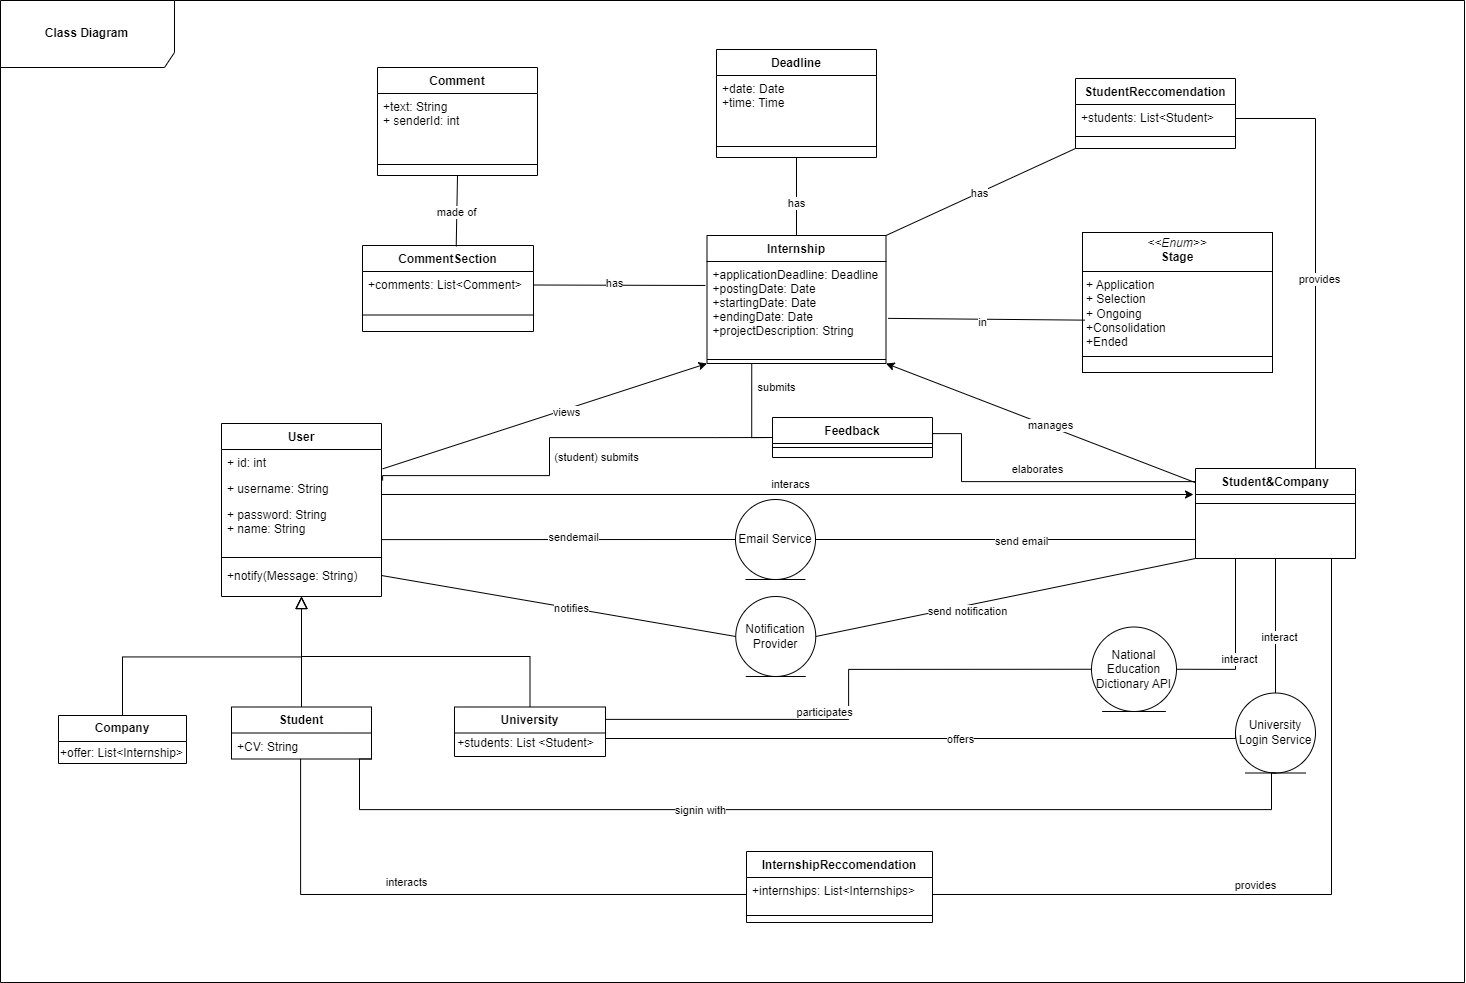
\includegraphics[scale = 0.30]{figures/Class Diagram.drawio.png}
    \centering
\end{figure}
\subsubsection{State Charts}
The following section outlines the key component (Internship) of the Student\&Company (S\&C) system and its evolution across different phases. To illustrate this, the UML State Chart is presented.
\begin{figure}[H]
    \centering
    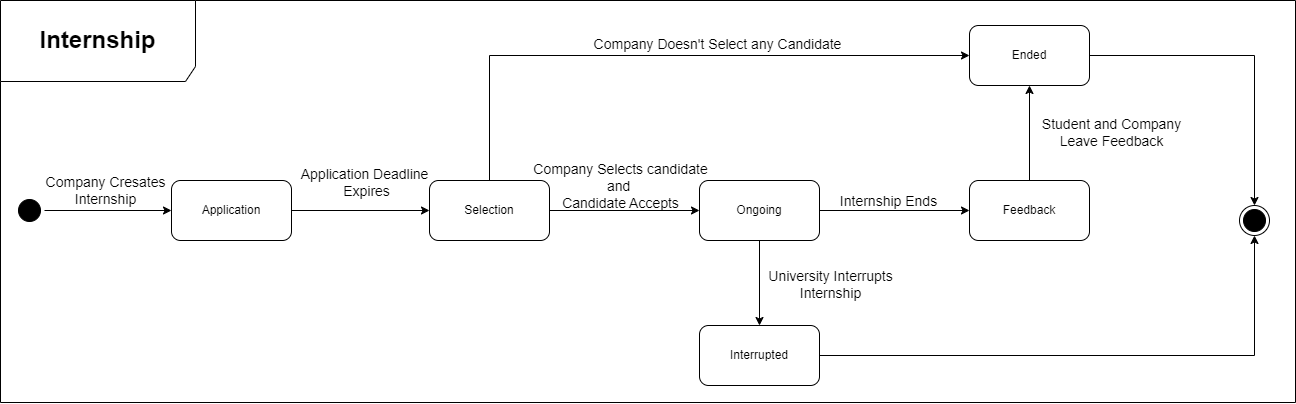
\includegraphics[scale = 0.30]{figures/StateCharts.drawio.png}
    \centering
\end{figure}
The diagram in question outlines the potential phases of an Internship. Posted by a Company, the Internship promptly enters the "Application" state, allowing Students to apply and Companies/Students to accept recommendations; in this state the company and the recommended students can provide feedback about the recommendation.
\\Following the closure of the application window, the system transitions the Internship to the "Selection" state, in which the Candidates are interviewed, selected and confirmed. 
\\In case no Candidate is confirmed, the Internship is archived and transitioned to the "Ended" state. Otherwise, the selected Candidate starts the interning period and the Internship is changed into the "Ongoing" state. 
\\While the Internship is "Ongoing" and the University responsible for the Student receives complaints, it may decide to terminate the Internship. In such cases, the Internship is moved to the "Interrupted" state and archived as is.
\\If the Internship ends without interruptions, before being archived, it waits for both the selected Candidate and the host Company to provide a feedback about the interning experience. The Internship is therefore placed in its "Feedback" state.
\\Only afterwards, the system closes the Internship, transitioning it in the "Ended" state and archiving it.


\subsection{Product Functions}

The platform \textbf{Students\&Companies} offers several key functions:

\begin{itemize}

    \item \textbf{Internship Advertisement:} 
    Companies can create and manage internship opportunities, specifying details such as descriptions and requirements .

    \item \textbf{Application Management:} 
    Students can browse internships and apply to those matching their skills and interests. Companies will review the applications based on the students' CV.

    \item \textbf{Recommendation System:} 
    The platform matches internships with students, facilitating the process for both sides.

    \item \textbf{Feedback Collection:} 
    Both Companies and Students can provide feedback, enabling continuous improvement of the platform.

    \item \textbf{Comments system:} 
    Both Companies and Students can write comments about the state of the on-going internship.

    \item \textbf{Interview Scheduling:} 
    Companies can schedule interviews with Students directly on the platform.

    \item \textbf{University Supervision:} 
    Universities can monitor their students' internship and can interrupt them if necessary.

\end{itemize}

\subsubsection{Requirements}
    \begin{itemize}
        \item \textbf{Requirement} 
        \item \textbf{R1} The system must allow a student who wants to register to sign up.
        \item \textbf{R2} The system must allow a company who wants to register to sign up.
        \item \textbf{R3} The system must allow a university who wants to register to sign up.
        \item \textbf{R4} The system must allow registered users to sign in using their credentials.
        \item \textbf{R6} The system must be able to send notifications to all users.
        \item \textbf{R7} The system must allow registered students to upload their CVs on the platform.
        \item \textbf{R8} The system must allow registered companies to post internship advertisements.
        \item \textbf{R9} The system must allow companies to review students' CVs and select candidates who meet their internship requirements.
        \item \textbf{R10} The system must allow students to review internship advertisements and select them if they wish to apply.
         \item \textbf{R11} The system must allow students to manually search for internship opportunities and save them to their favorites.
         \item \textbf{R12} The system must notify students when there are updates regarding the internships they applied for or accepted.
        \item \textbf{R13} The system must notify a student and a company that accept each other.
        \item \textbf{R14} The system must allow companies to choose a suitable date for the interview, but only after a match is done.
        \item \textbf{R15} The system must schedule an interview at the date and time specified by the company and notify the selected students.
        \item \textbf{R16} The system must recommend a student and a internship to each other if the student's profile matches the needs of the company. 
        \item \textbf{R17} The system must allow companies to offer internship proposals to selected students after the interview process is completed.
        \item \textbf{R18}The system must allow companies and students to give feedback at the end of the internship in which they took part.
        \item \textbf{R19} The system must allow the student and company who got recommended to each other to give feedback about the recommendation.
        \item \textbf{R20} The system must provide a suggested template to users for improving their CV or project description.
        \item \textbf{R21} The system must notify students when there are updates regarding the results of the internships they have applied for.
        \item \textbf{R22} The system must allow selected students to accept or decline internship proposal sent by companies.    
        \item \textbf{R24} The system must allow companies to view and manage applications for the internships they have posted.
        \item \textbf{R25} The system must allow students to view all details about the internships they have applied for, such as completion status, and deadlines.
        \item \textbf{R27} The system must allow universities to follow internship processes, handle complaints raised by students, and interrupt an internship if necessary.
        
        \end{itemize}
\subsection{User characteristics}
     A User can be one of three types: Student, University, Company. Each role has access to distinct functionalities and is driven by different motivations.
     \begin{itemize}
        \item Students: They are students of some university; they want to apply for internships, either helped by the recommendations from the platform or by looking for internship themselves. If they have something to say about their on-going internship, they can make observations or complaints in the platform.
        \item Companies: They want to recruit students for their internship projects. They are aided in the selection process from the platform. They might want to make observations or complaints about the hired student.
        \item Universities: They want to manage their students' on-going internship, handling their complaints or the ones coming from the company of the internship.     
     \end{itemize}
\subsection{Assumptions, dependencies and constraints}
This section serves as a comprehensive overview of critical factors which must be considered during the implementation of the platform. It consolidates the foundational assumptions made during project planning and highlights eventual dependencies.
\subsubsection{Domain Assumptions}
    \begin{itemize}
        \item D1 The User must have a working Internet connection.
        \item D2 Students are enrolled in a registered university as students of any kind.
        \item D3 The User registering is either a student, a university or a company.
        \item D4 A university needs to be registered for its students to link their accounts and start applying for internships.
        \item D5 The university profiles are registered using the university email from the ones of the specialized staff (like career centers, internship coordinators, etc.) for the task.
        \item D6 The student registers using his university mail.

    \end{itemize}
\subsubsection{Dependencies}
An EmailService is needed, because in the registration process a verifcation email must be sent by the system to let Users successfully sign up.
\\A UniversityLoginService is needed for creating a connection between the university students' profiles and the university profile.
\\A NotificationProvider is needed, either implemented or integrated.
\\A NationalEducationDictionaryService is needed to check if the university registering actually exists or not.

\section{Specific Requirements}
\subsection{External Interface Requirements}
In this section, the system aims to develop a user-friendly interface that aligns with the goals, requirements, and scenarios outlined in Sections 1.1.1, 2.2.1, and 2.1.1, respectively. In addition, the system enables users to access the interface through any web browser on personal computers and utilize the general functions specified in section 2.2.
\subsubsection{User Interfaces}
\begin{figure}[H]
    \centering
    
\includegraphics[scale = 0.40]{figures/UserInterfaces/General/Entrance.png}
    \caption{Entrance}
    \centering
\end{figure}
\begin{figure}[H]
    \centering
    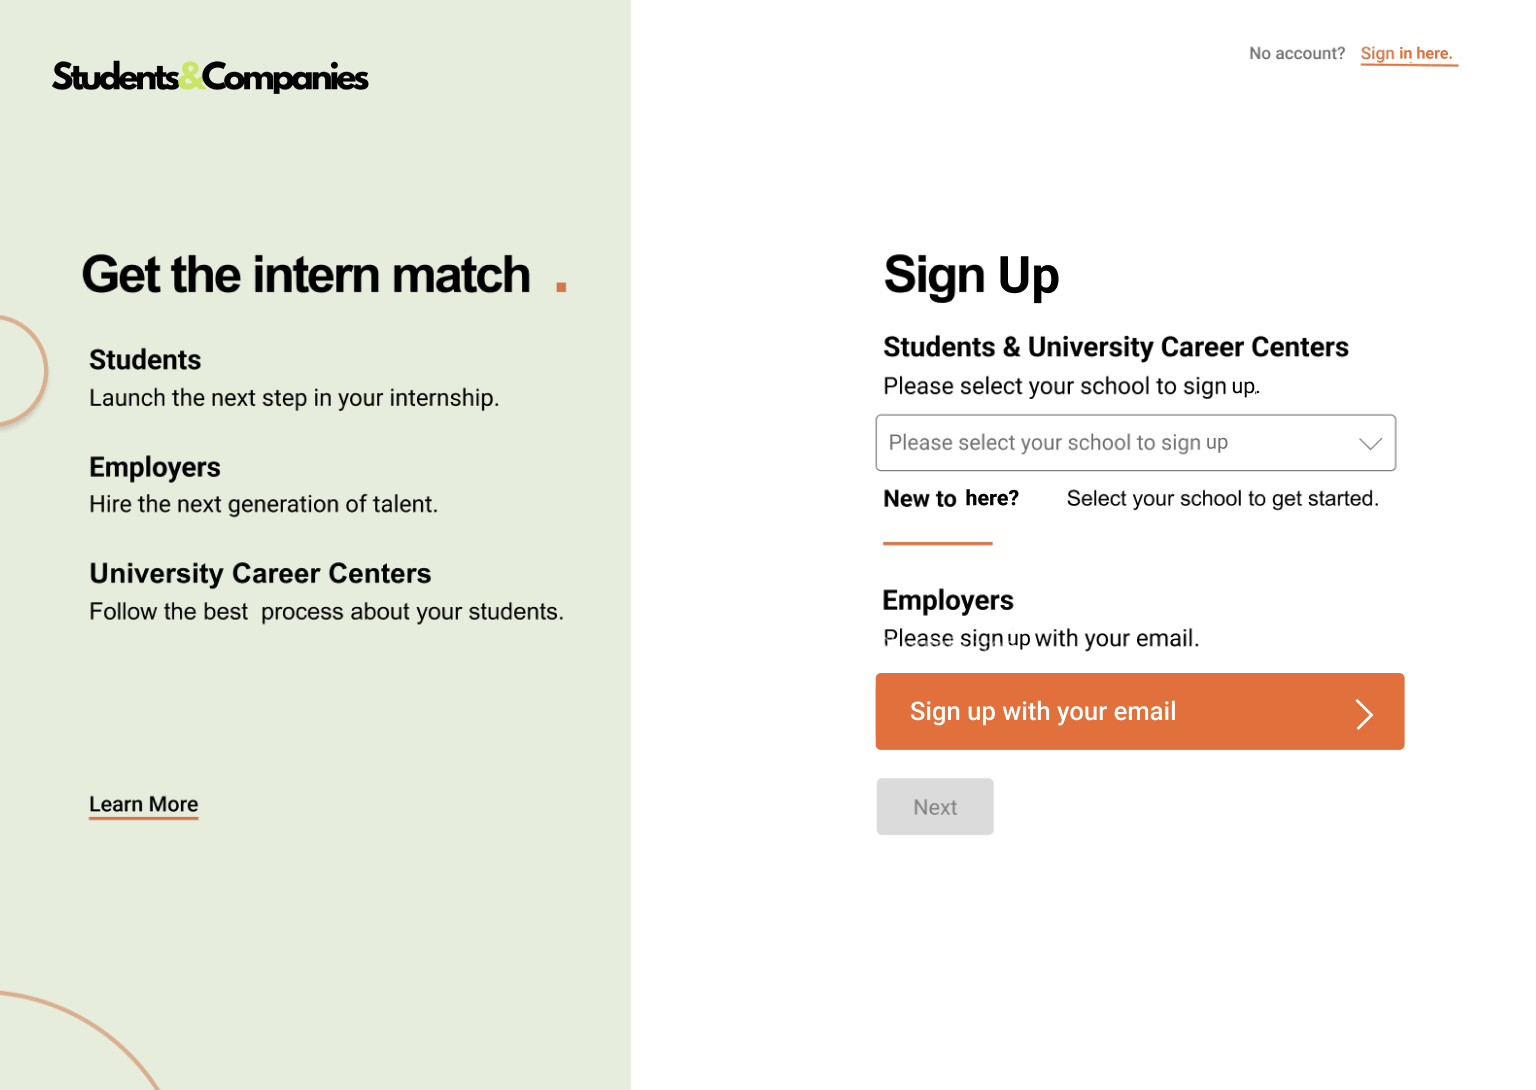
\includegraphics[scale = 0.40]{figures/UserInterfaces/General/HomeSignUp.png}
    \caption{Home Sign Up Page}
    \centering
\end{figure}
\begin{figure}[H]
    \centering
    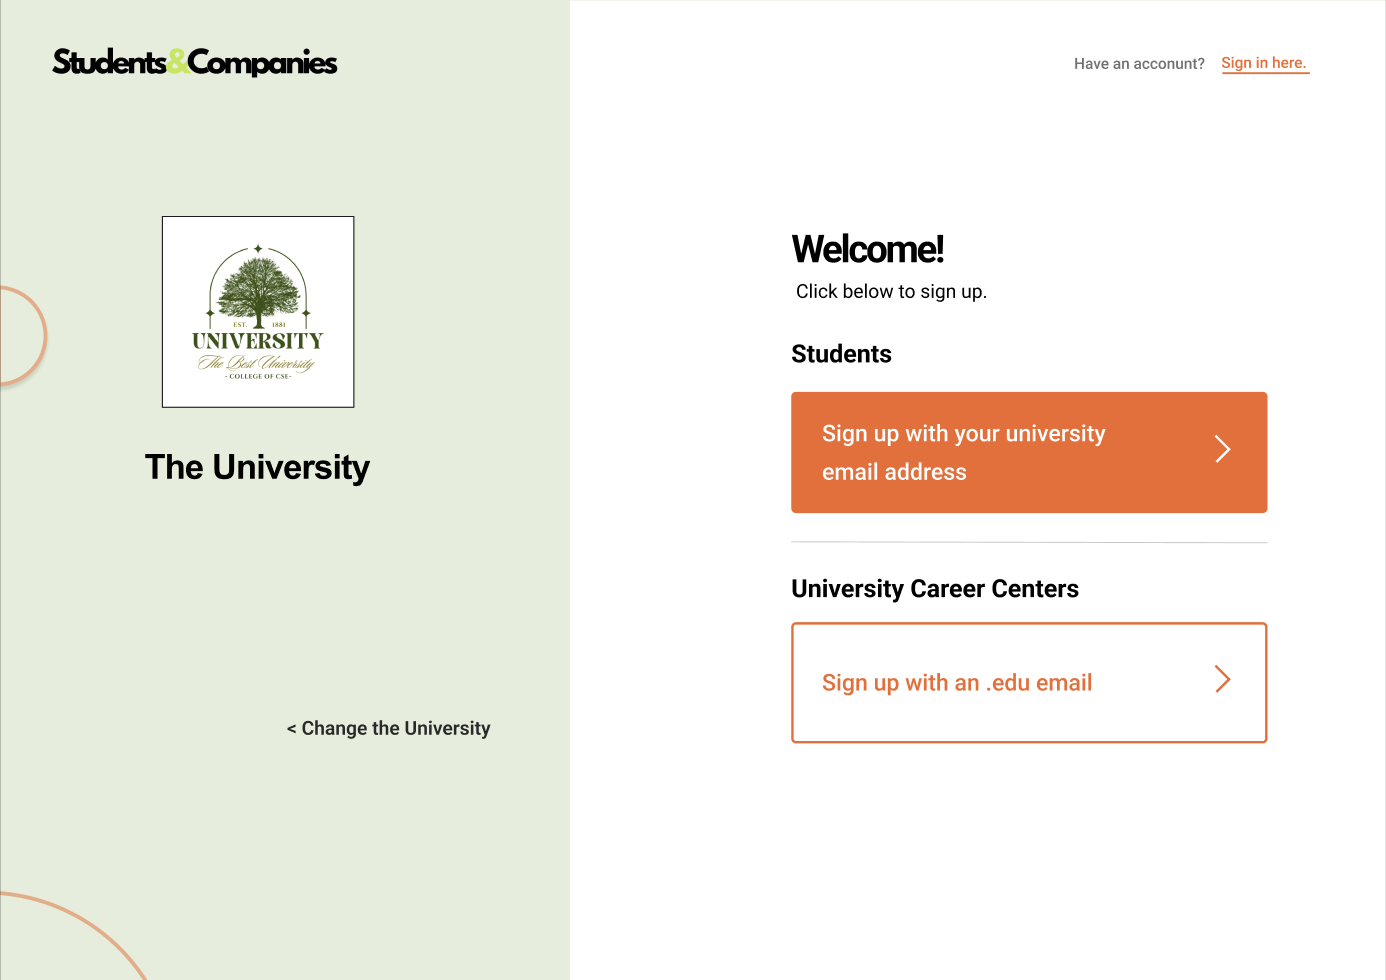
\includegraphics[scale = 0.40]{figures/UserInterfaces/General/SUSignUp.png}
    \caption{Student \& University Sign Up}
    \centering
\end{figure}
\begin{figure}[H]
    \centering
    
\includegraphics[scale = 0.45]{figures/UserInterfaces/General/StudentSignUp.png}
    \caption{Student Sign Up Page}
    \centering
\end{figure}
\begin{figure}[H]
    \centering
    
\includegraphics[scale = 0.42]{figures/UserInterfaces/General/StudentUploadCV.png}
    \caption{Student Upload CV}
    \centering
\end{figure}
\begin{figure}[H]
    \centering
    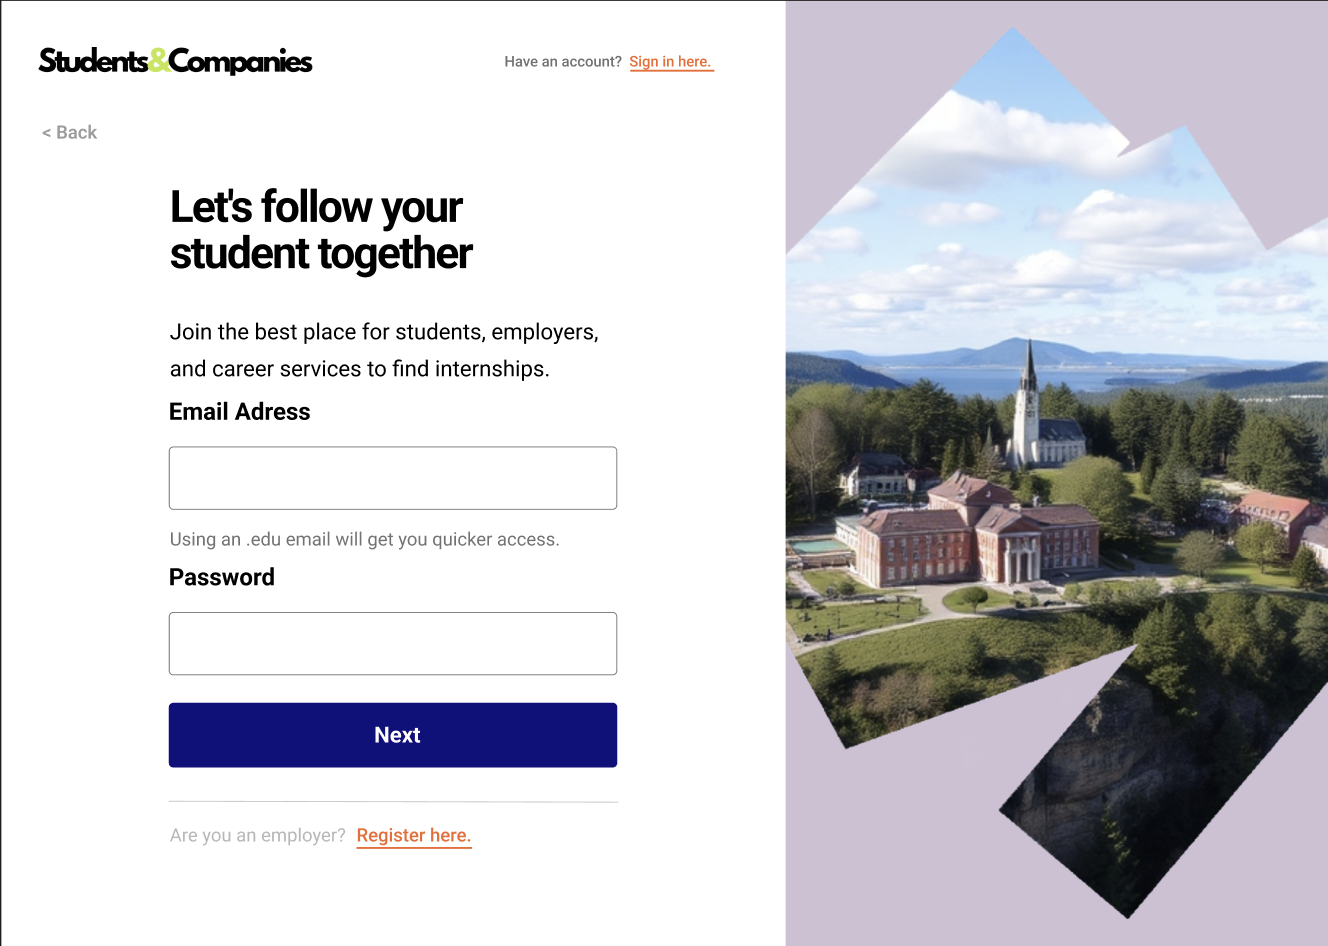
\includegraphics[scale = 0.45]{figures/UserInterfaces/General/UniversitySignUp.png}
    \caption{University Sign Up Page}
    \centering
\end{figure}
\begin{figure}[H]
    \centering
    
\includegraphics[scale = 0.45]{figures/UserInterfaces/General/EmployerSignUp.png}
    \caption{Employer Sign Up Page}
    \centering
\end{figure}
\begin{figure}[H]
    \centering
    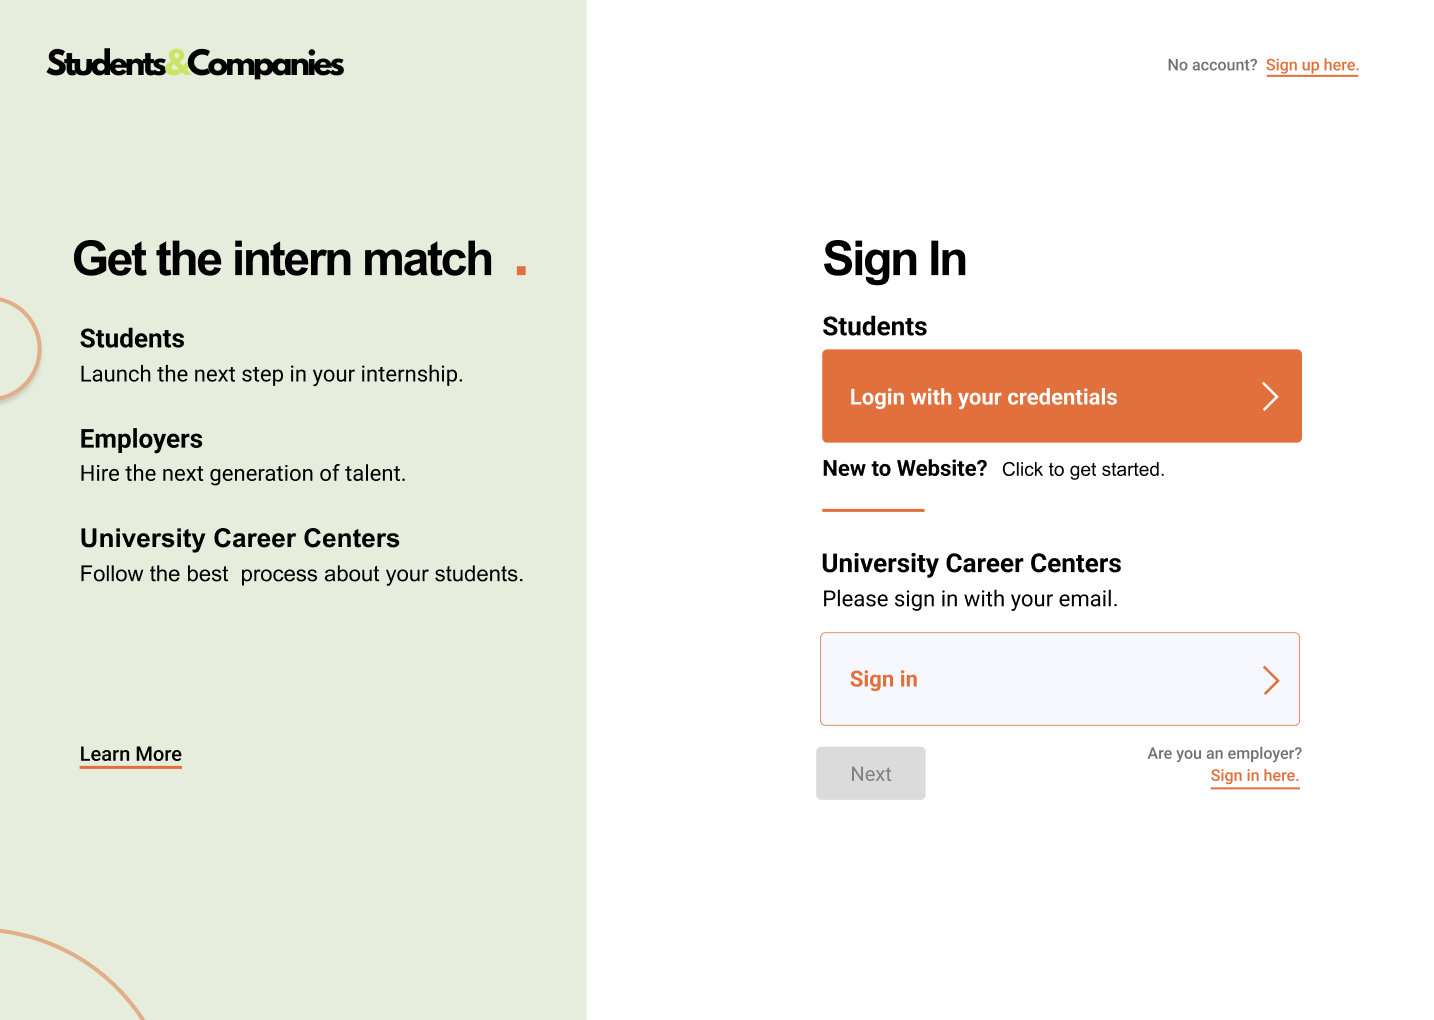
\includegraphics[scale = 0.42]{figures/UserInterfaces/General/HomeSignIn.png}
    \caption{Student \& University Home Sign In}
     \centering
\end{figure}

\begin{figure}[H]
    \centering
    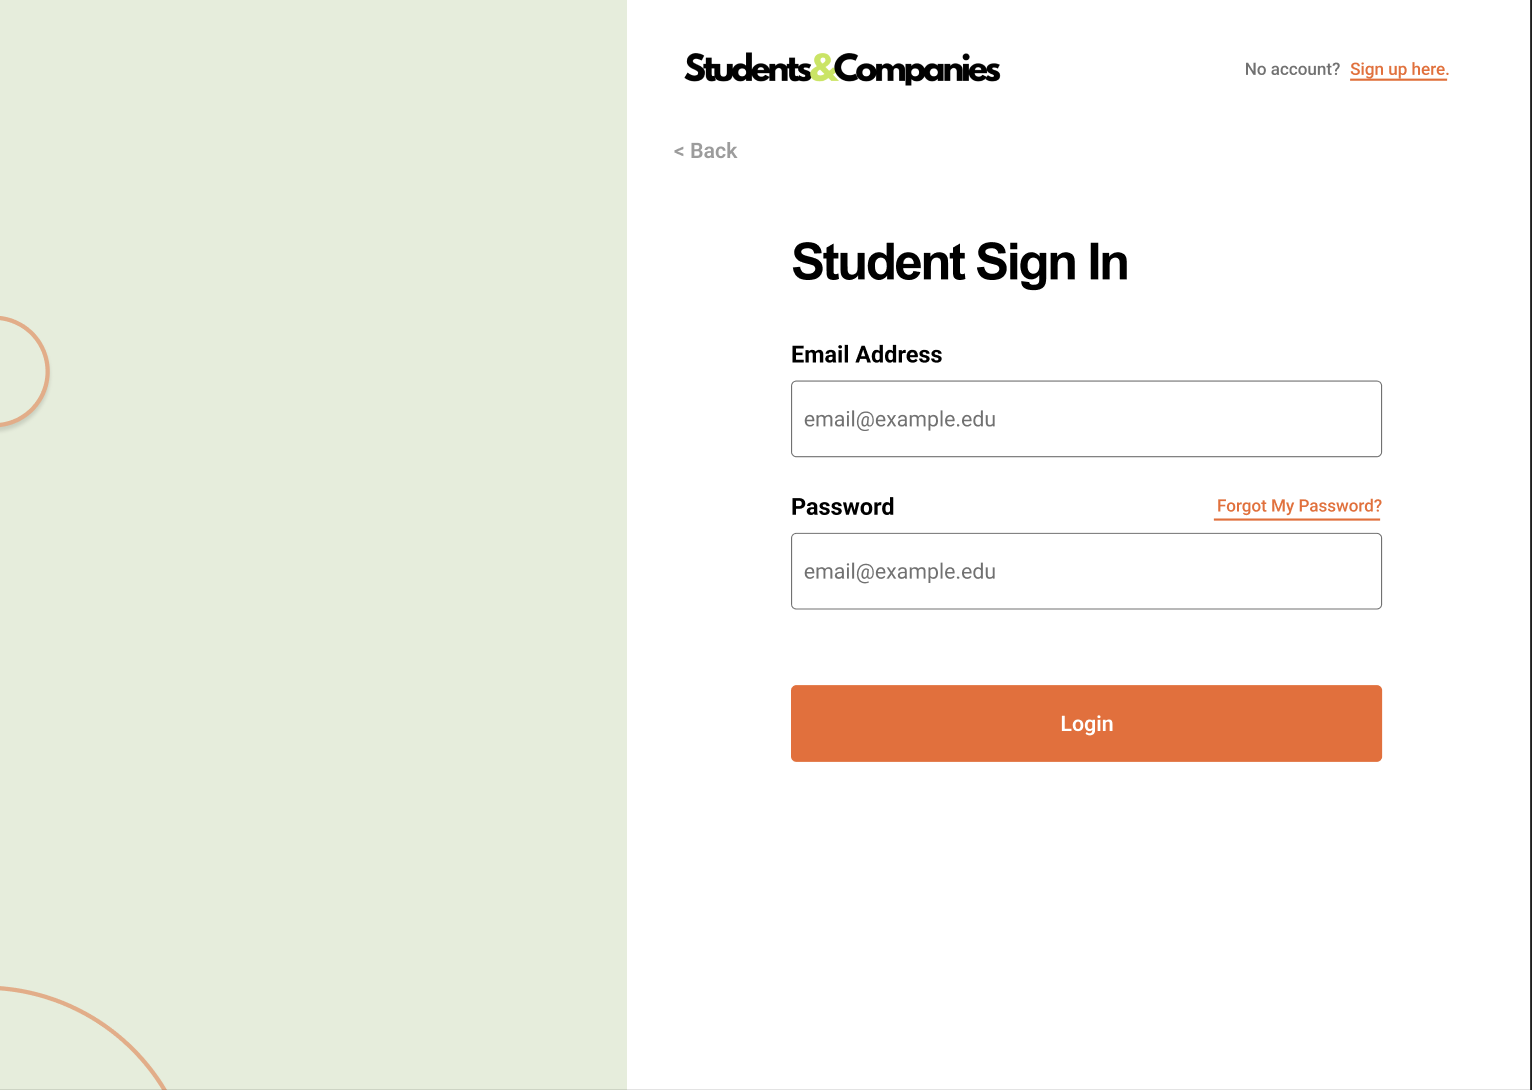
\includegraphics[scale = 0.40]{figures/UserInterfaces/General/StudentSignIn.png}
    \caption{Student Sign In}
     \centering
\end{figure}
\begin{figure}[H]
    \centering
\begin{figure}[H]
    \centering
    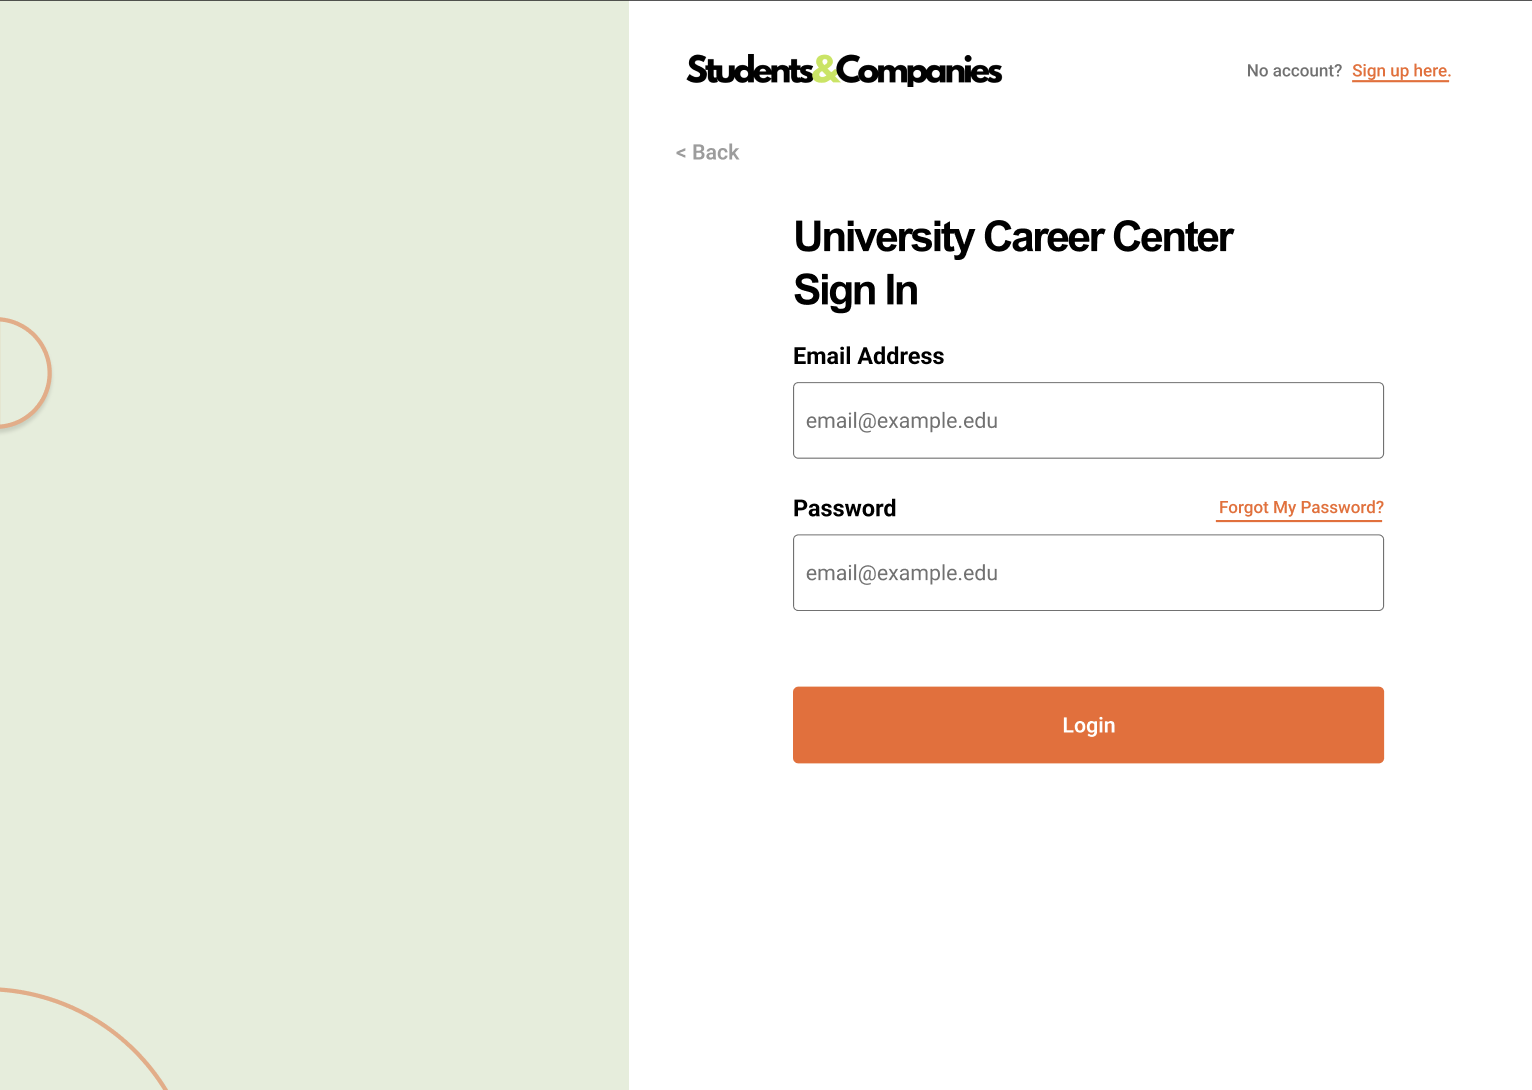
\includegraphics[scale = 0.40]{figures/UserInterfaces/General/UniversitySignIn.png}
    \caption{University Sign In}
     \centering
\end{figure}
    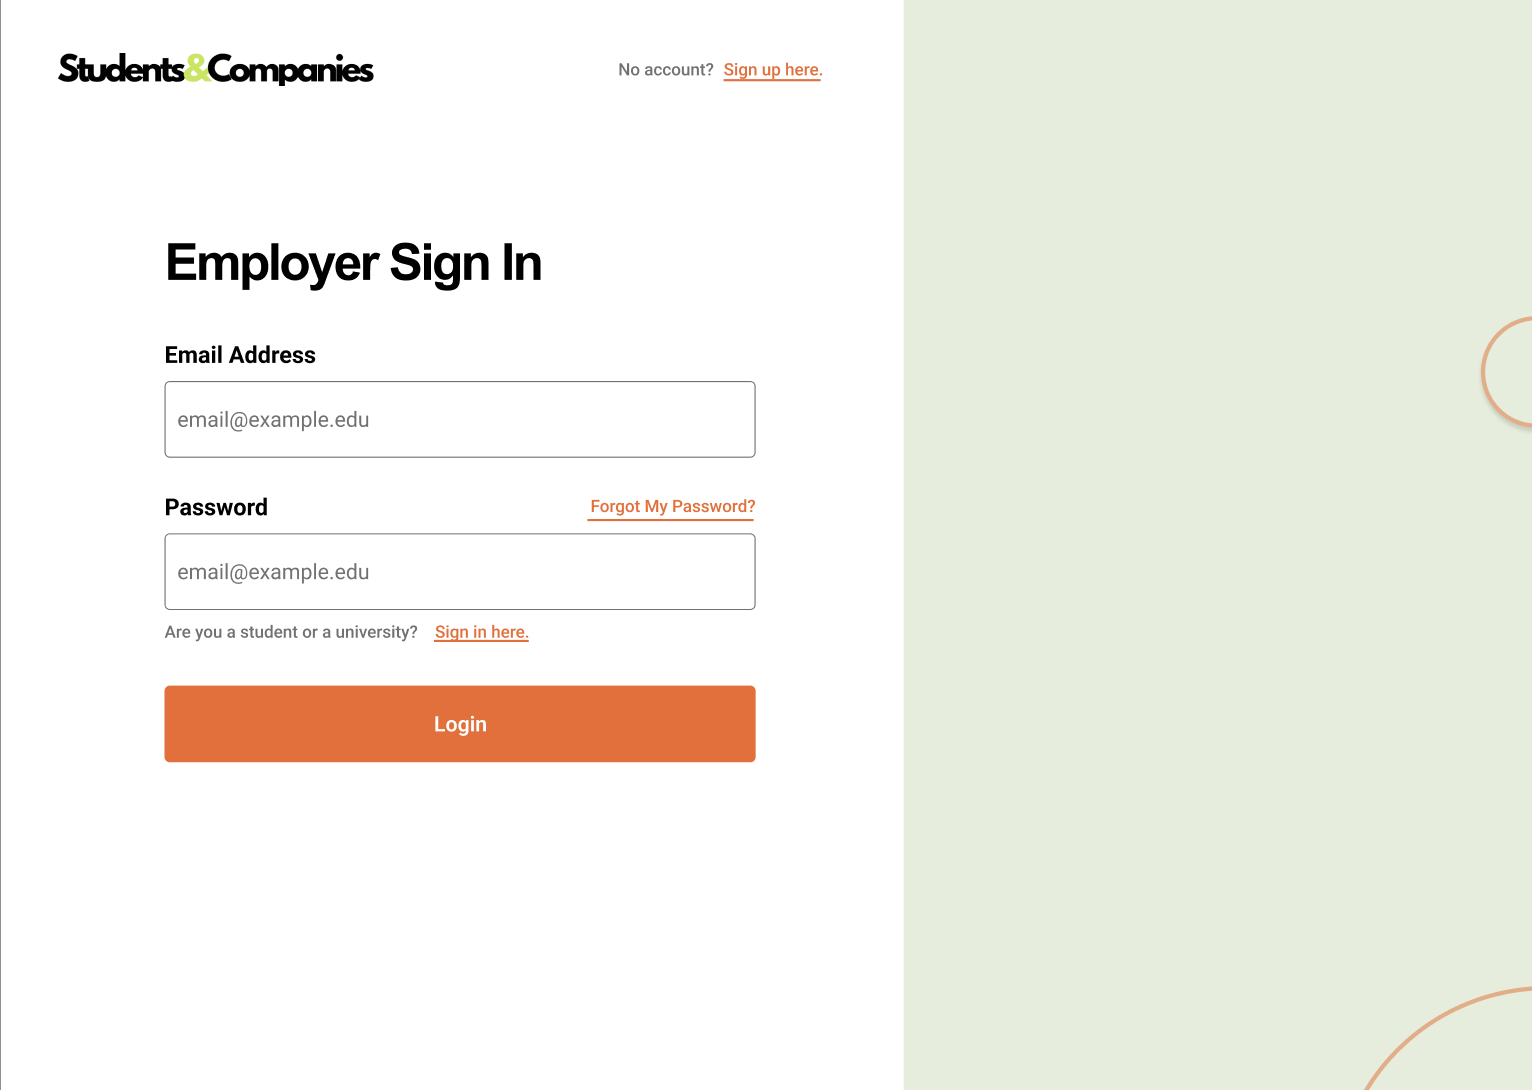
\includegraphics[scale = 0.40]{figures/UserInterfaces/General/EmployerSignIn.png}
    \caption{Employer Sign In}
     \centering
\end{figure}

\begin{figure}[H]
    \centering
    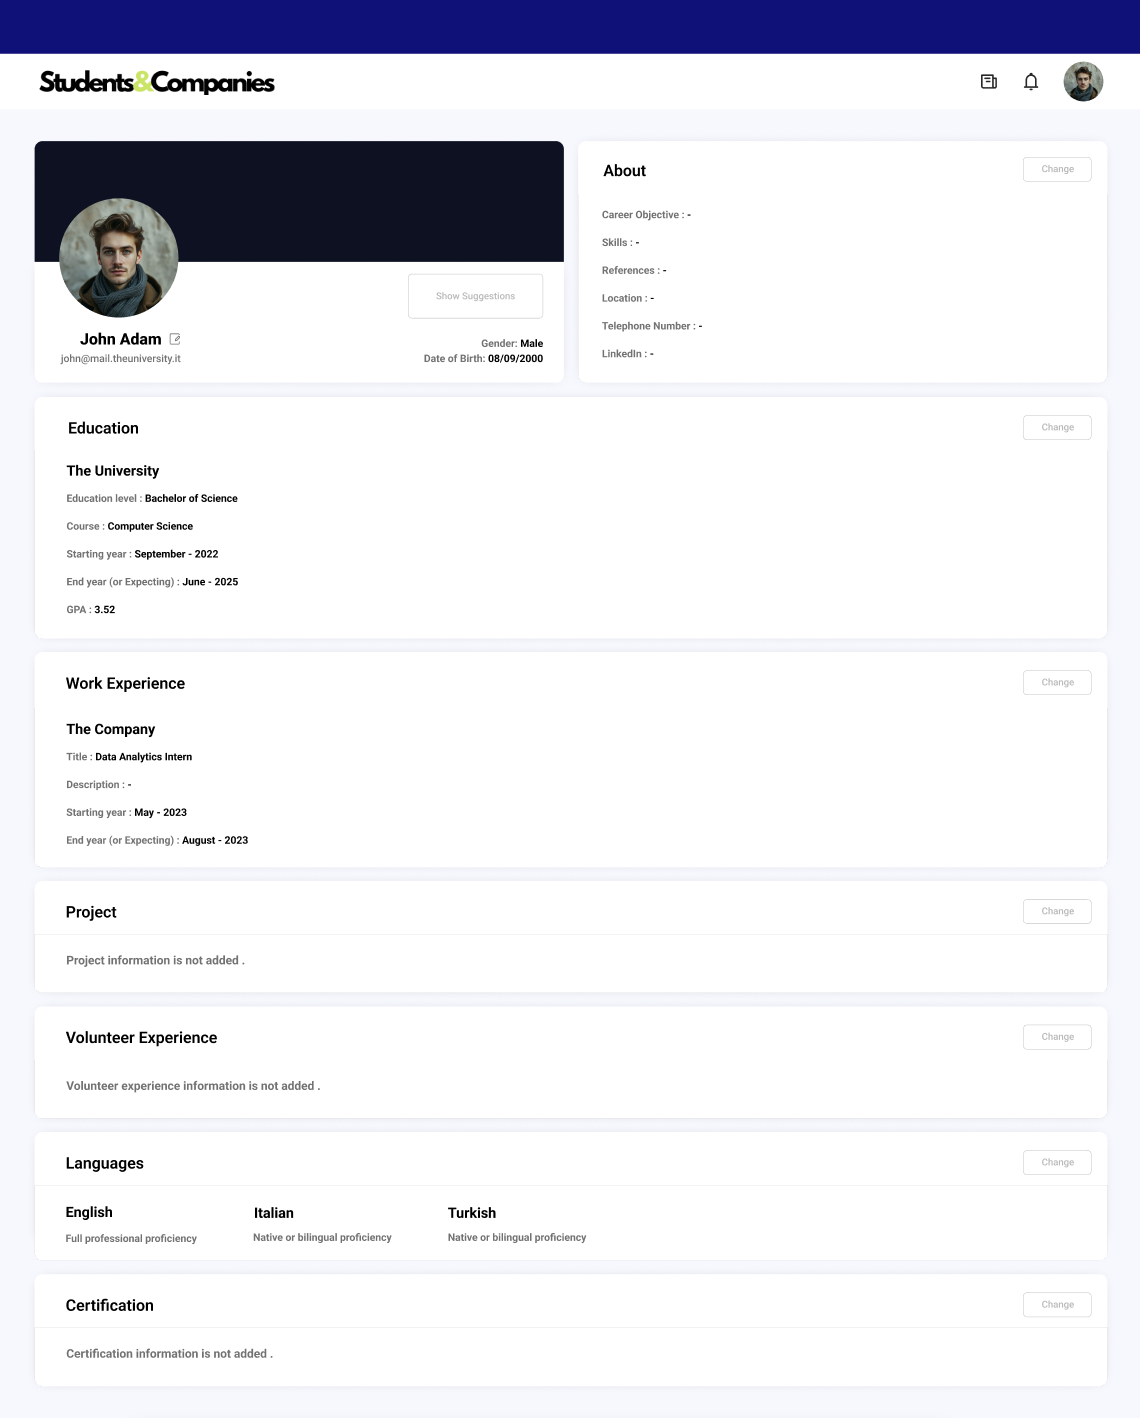
\includegraphics[scale = 0.35
    ]{figures/UserInterfaces/Student/Profile.png}
    \caption{Student Profile Details}
     \centering
\end{figure}
    \begin{figure}[H]
    \centering
    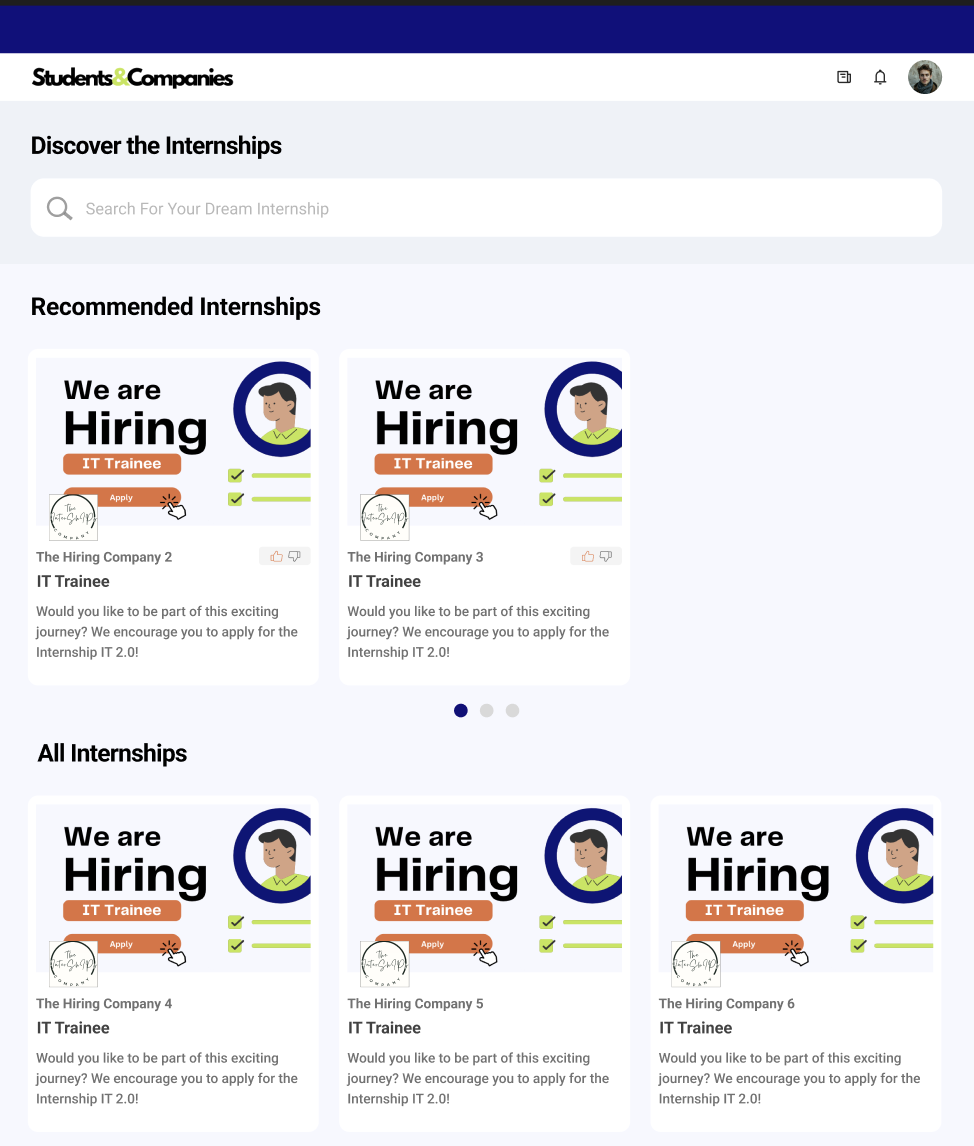
\includegraphics[scale = 0.40]{figures/UserInterfaces/Student/HomePage1.png}
    \caption{Student Home Page 1}
     \centering
\end{figure}

\begin{figure}[H]
    \centering
    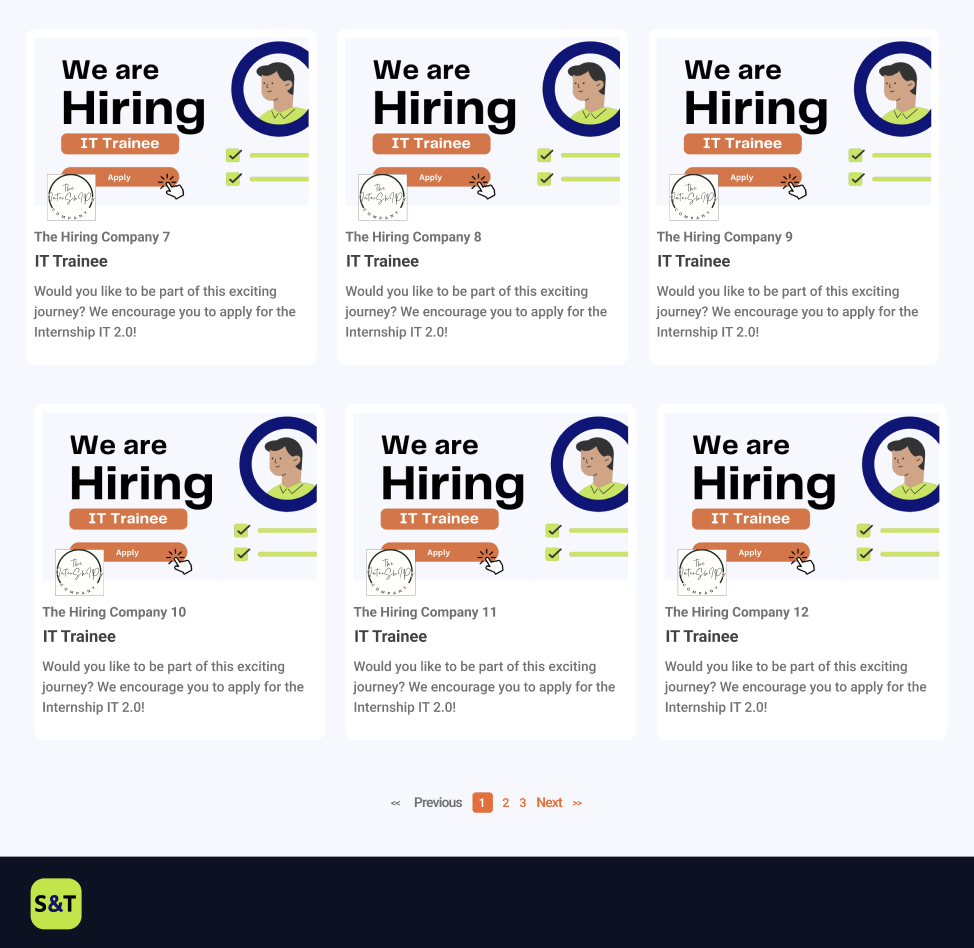
\includegraphics[scale = 0.40]{figures/UserInterfaces/Student/HomePage2.png}
    \caption{Student Home Page 2}
     \centering
\end{figure}

\begin{figure}[H]
    \centering
    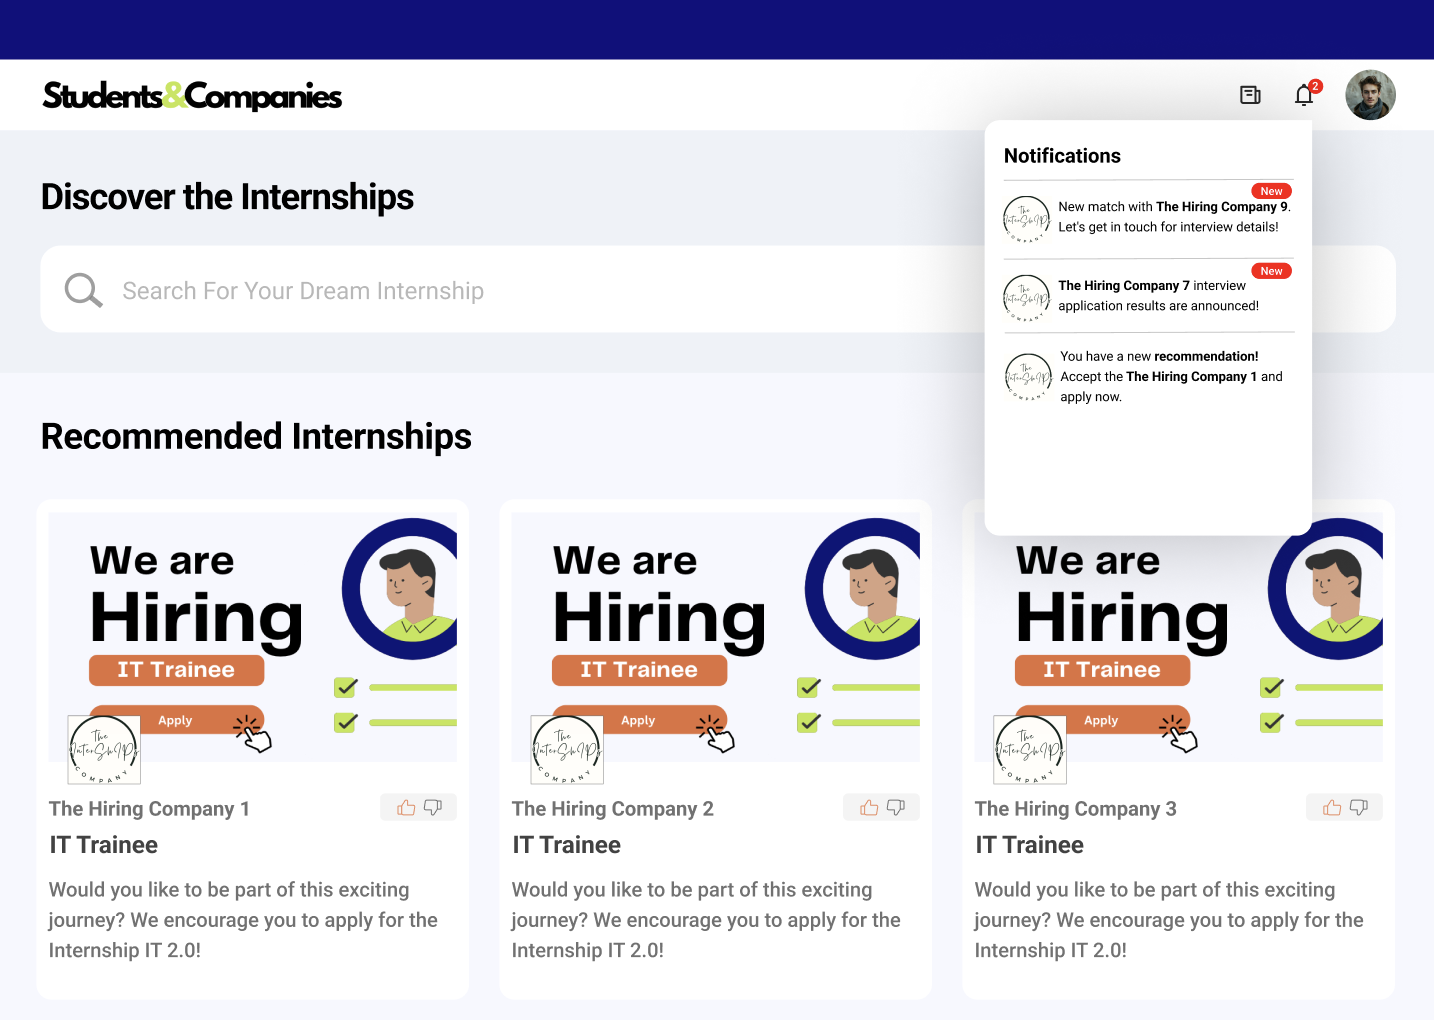
\includegraphics[scale = 0.435]{figures/UserInterfaces/Student/Notifications.png}
    \caption{Student Notifications}
     \centering
\end{figure}

\begin{figure}[H]
    \centering
    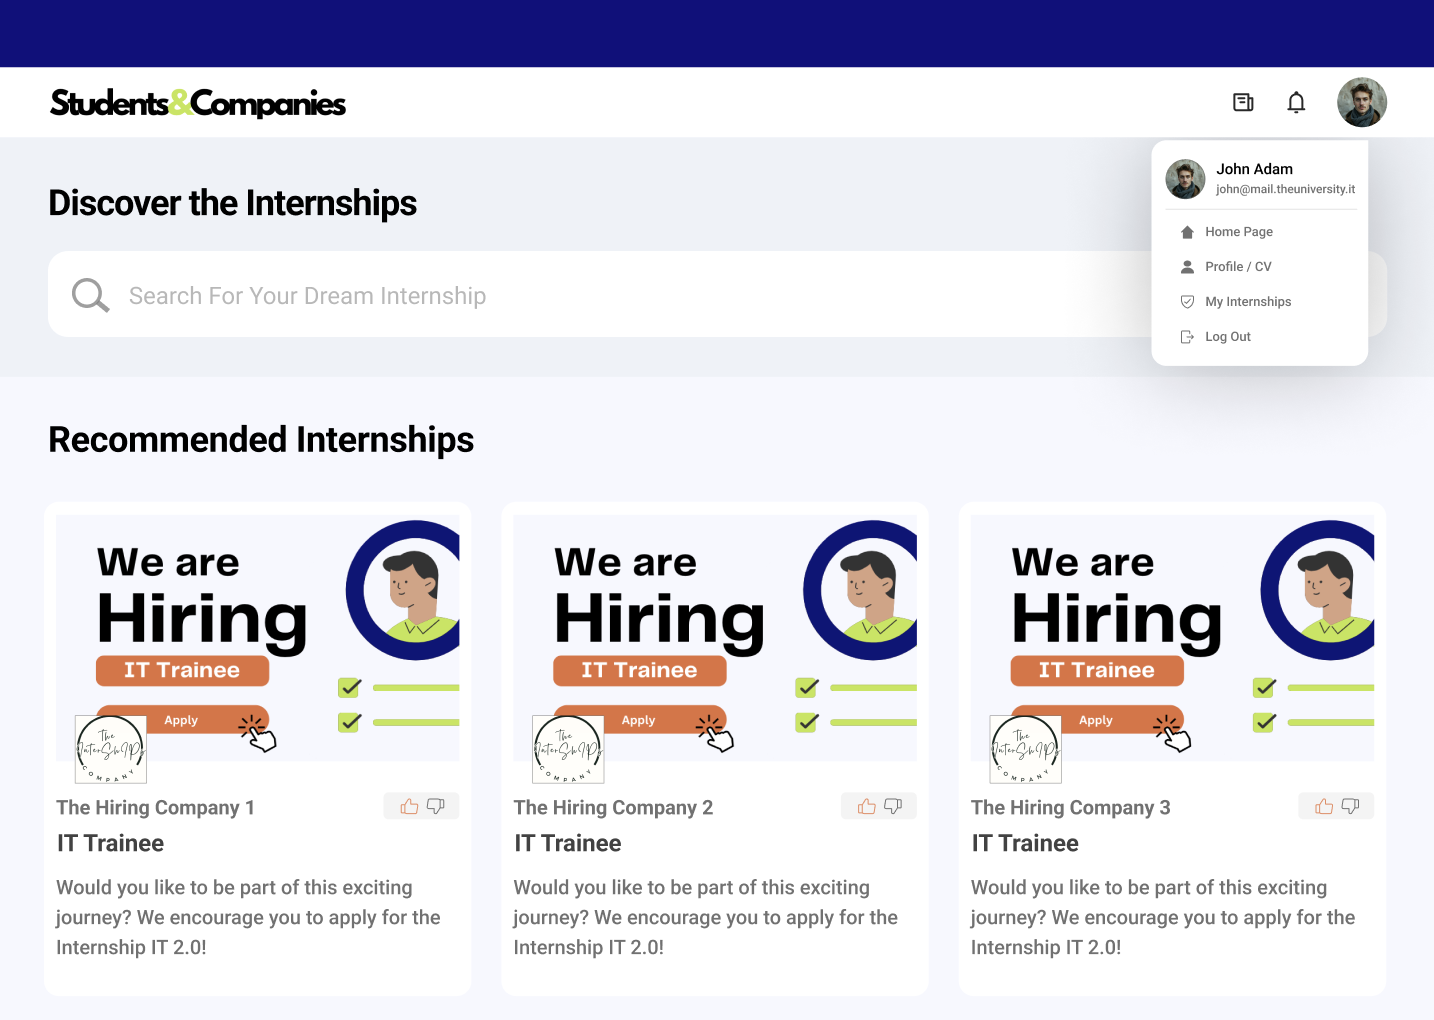
\includegraphics[scale = 0.40]{figures/UserInterfaces/Student/ProfileMenu.png}
    \caption{Student Profile Menu}
     \centering
\end{figure}

\begin{figure}[H]
    \centering
    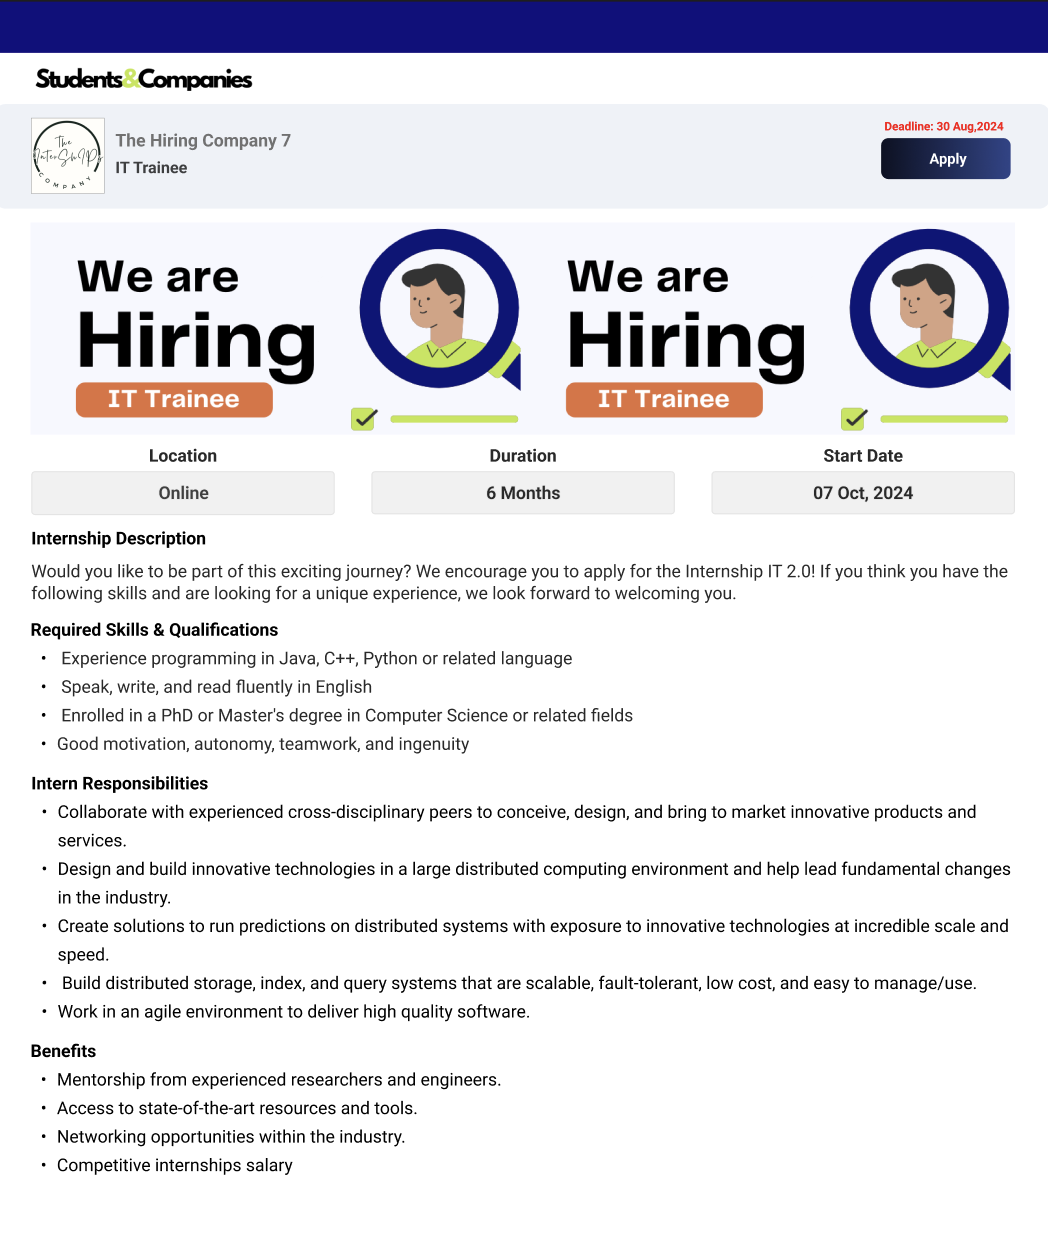
\includegraphics[scale = 0.65]{figures/UserInterfaces/Student/AdvertisementPage.png}
    \caption{Advertisement Details Page}
     \centering
\end{figure}

\begin{figure}[H]
    \centering
    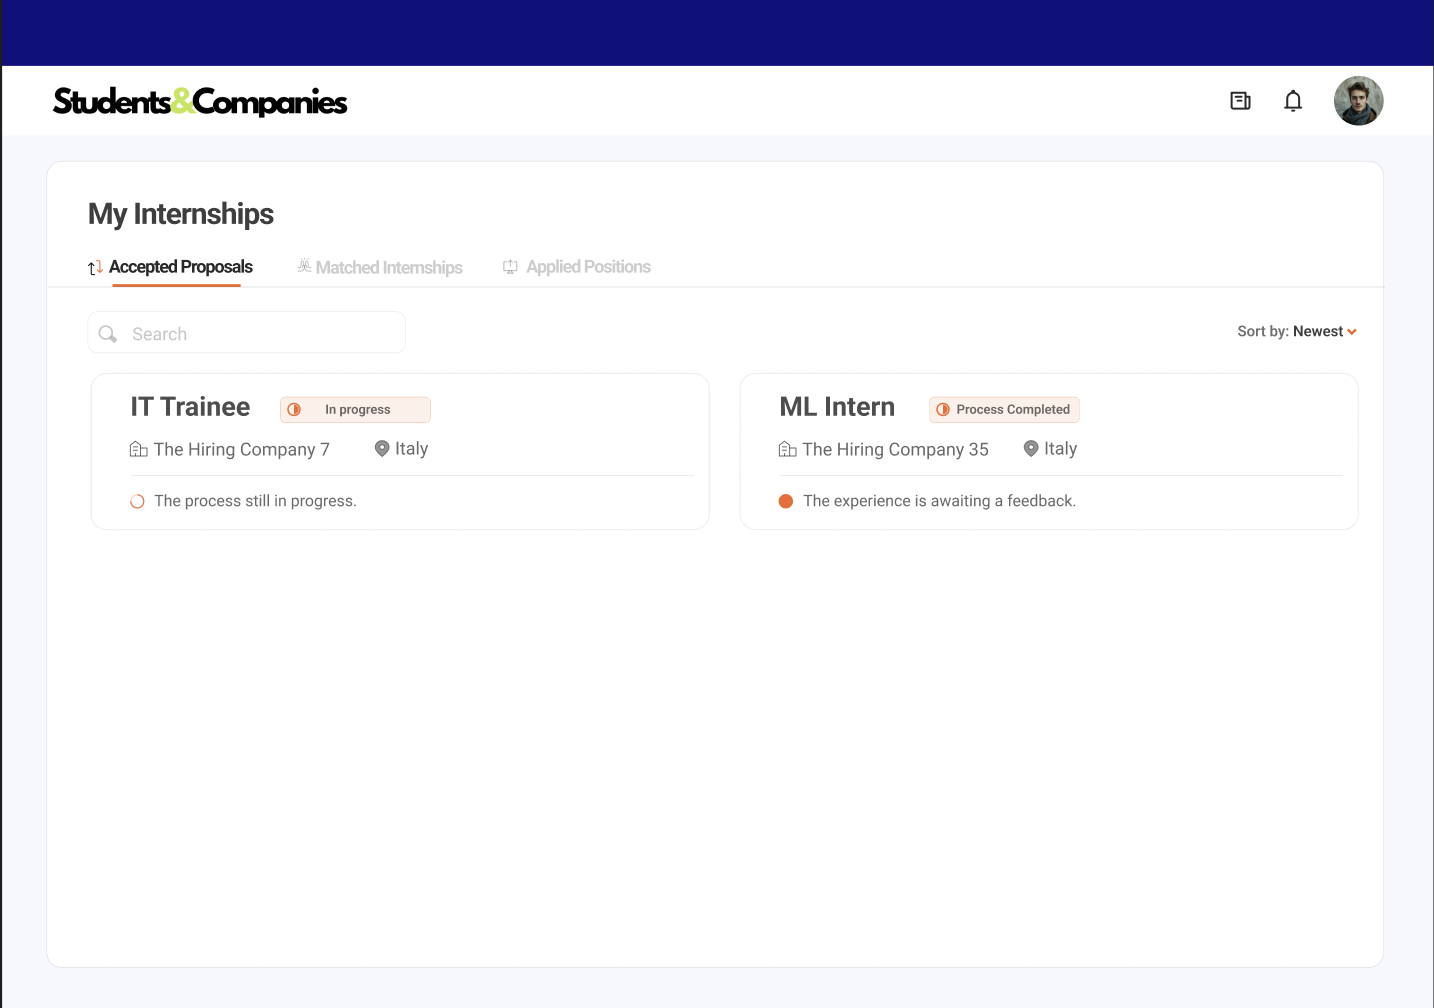
\includegraphics[scale = 0.42]{figures/UserInterfaces/Student/AcceptedProposals.png}
    \caption{Student Accepted Internships}
     \centering
\end{figure}
\begin{figure}[H]
    \centering
    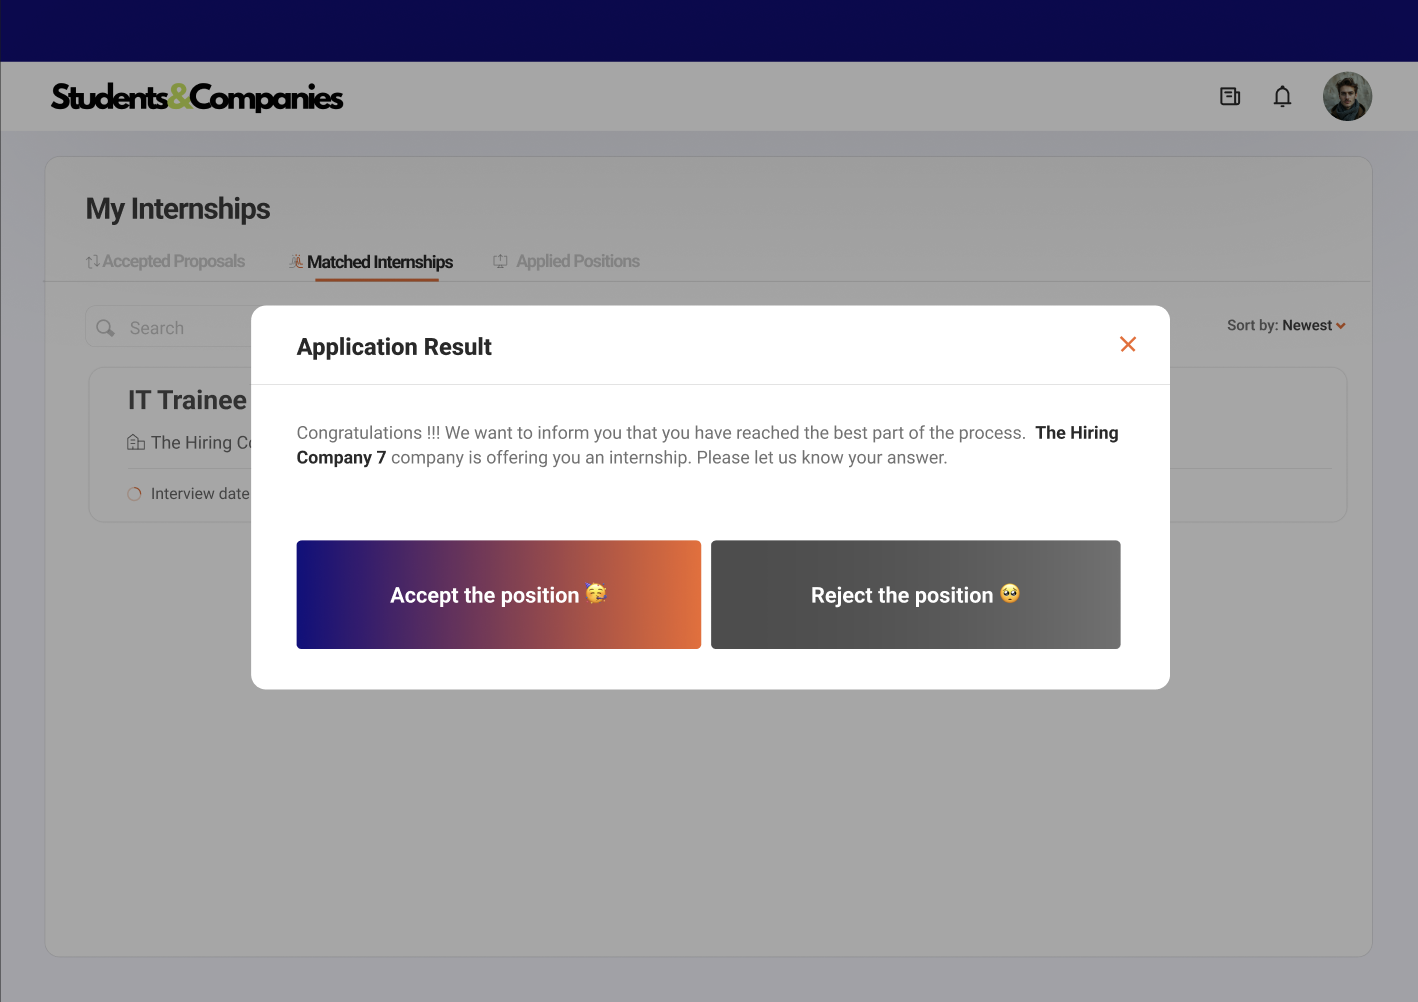
\includegraphics[scale = 0.42]{figures/UserInterfaces/Student/AcceptPop-up.png}
    \caption{Accepting the position}
     \centering
\end{figure}


\begin{figure}[H]
    \centering
    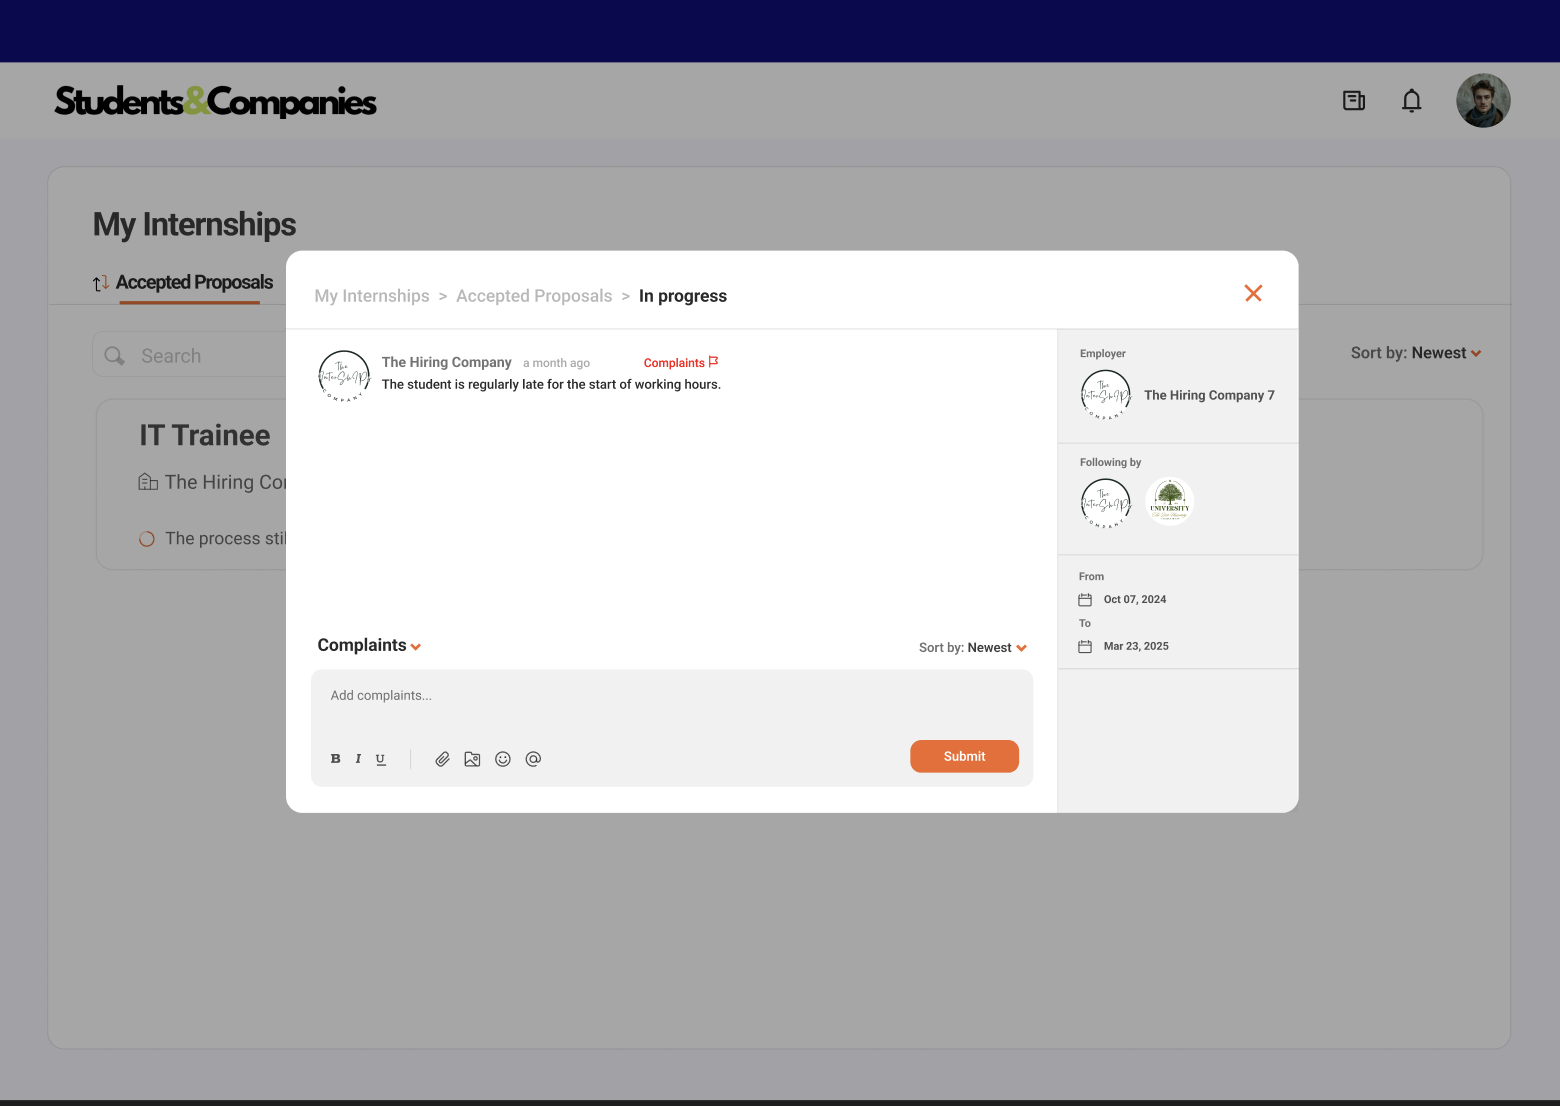
\includegraphics[scale = 0.42]{figures/UserInterfaces/Student/StudentComplaints.png}
    \caption{Student Ongoing Internship Complaints}
     \centering
\end{figure}
\begin{figure}[H]
    \centering
    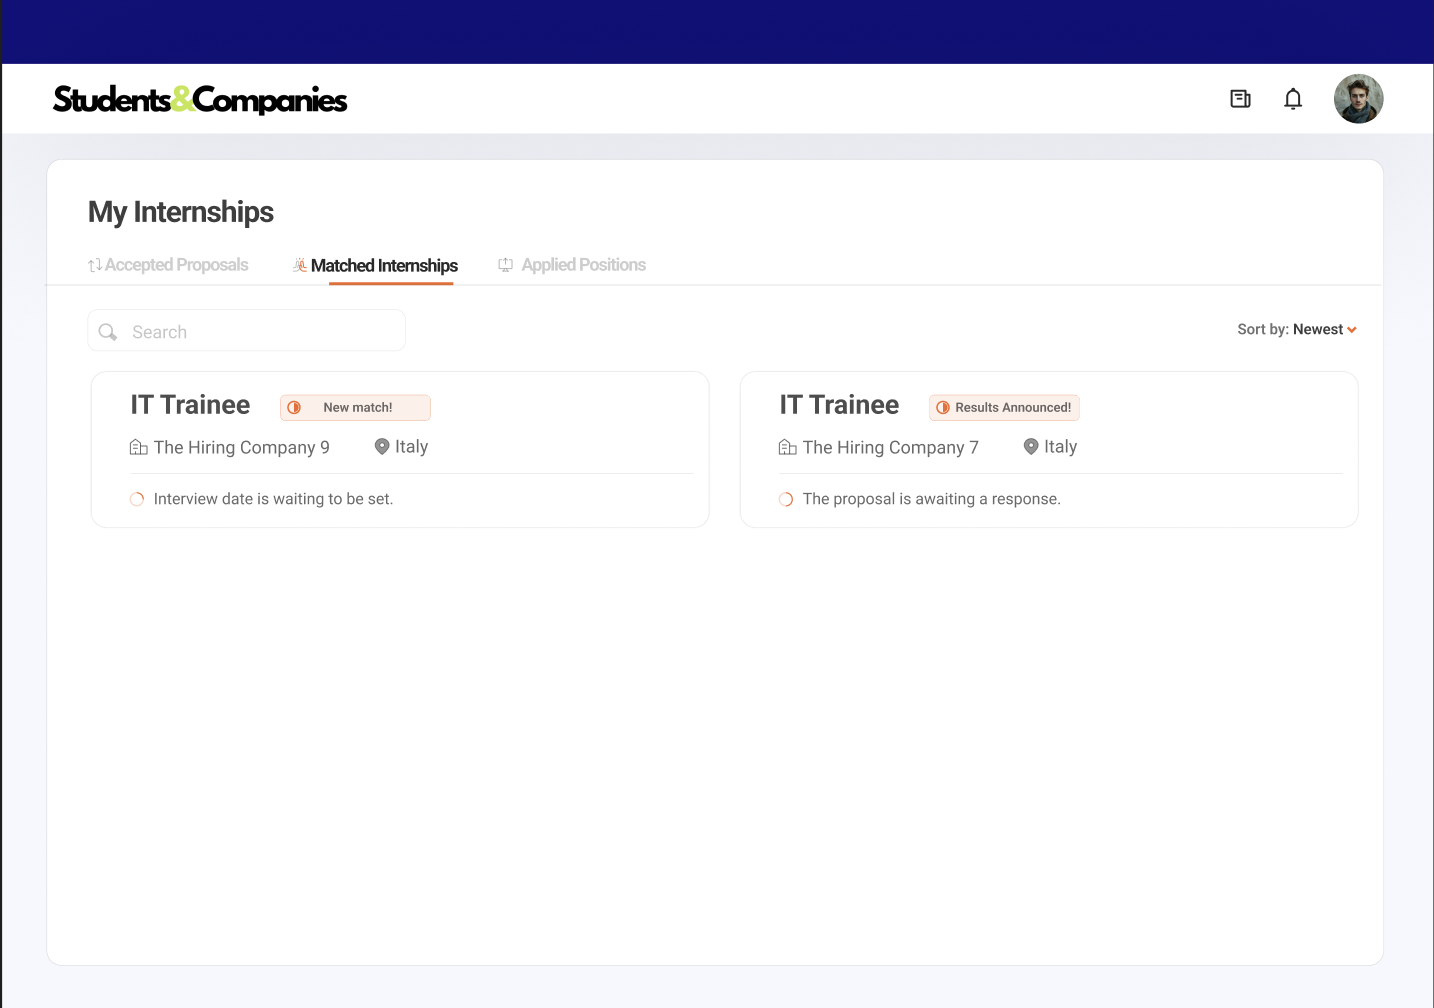
\includegraphics[scale = 0.42]{figures/UserInterfaces/Student/MatchedInternships.png}
    \caption{Student Matched Internships}
     \centering
\end{figure}

\begin{figure}[H]
    \centering
    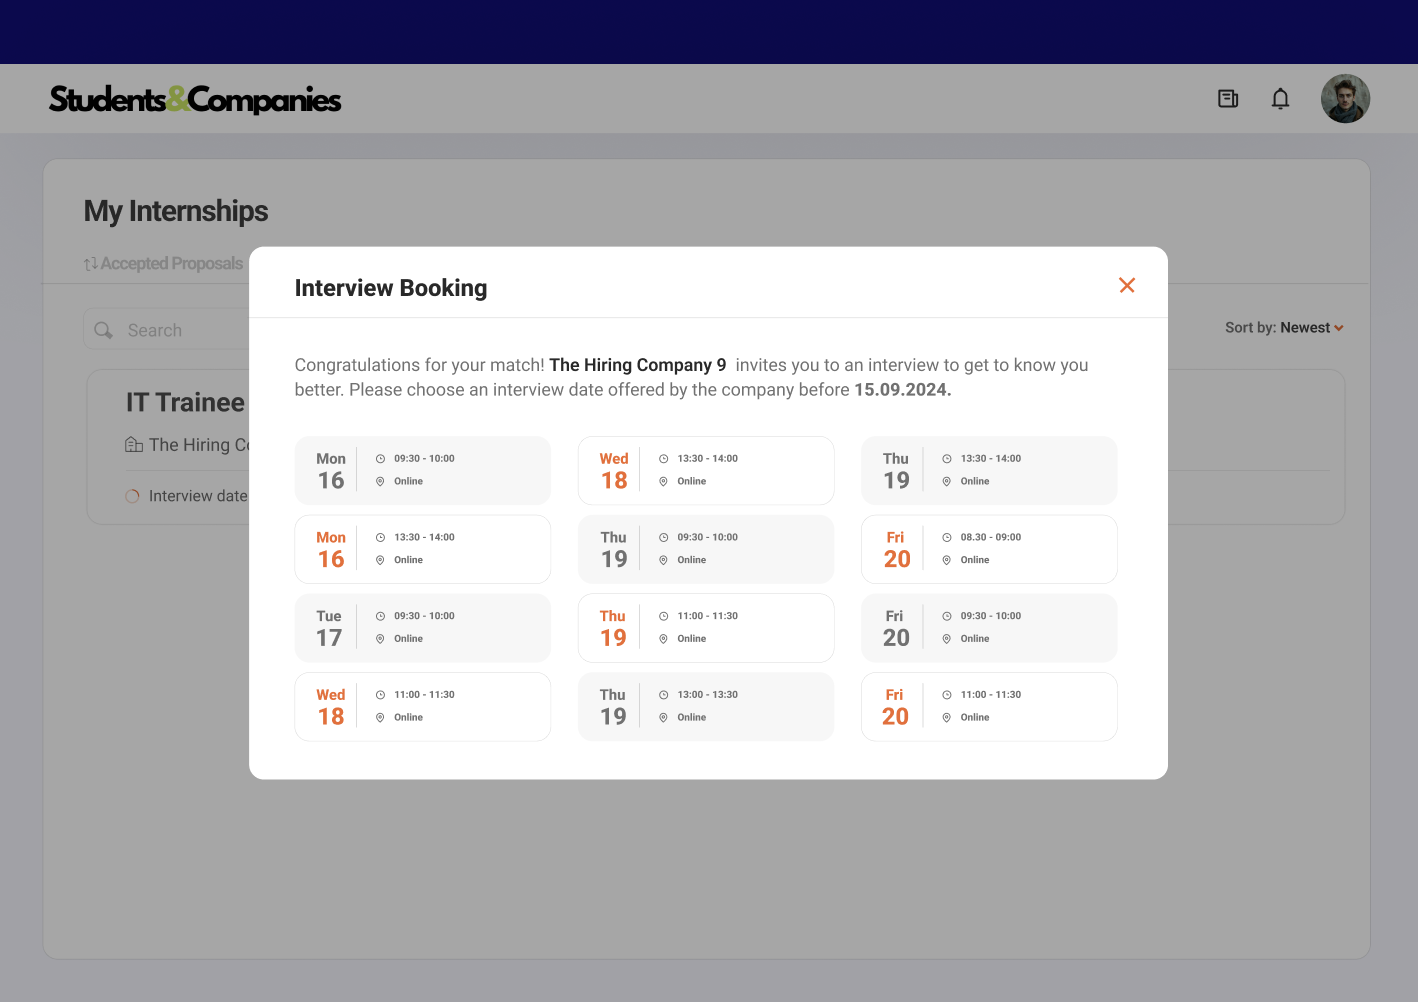
\includegraphics[scale = 0.42]{figures/UserInterfaces/Student/BookingPop-up.png}
    \caption{Student Interview Schedule}
     \centering
\end{figure}

\begin{figure}[H]
    \centering
    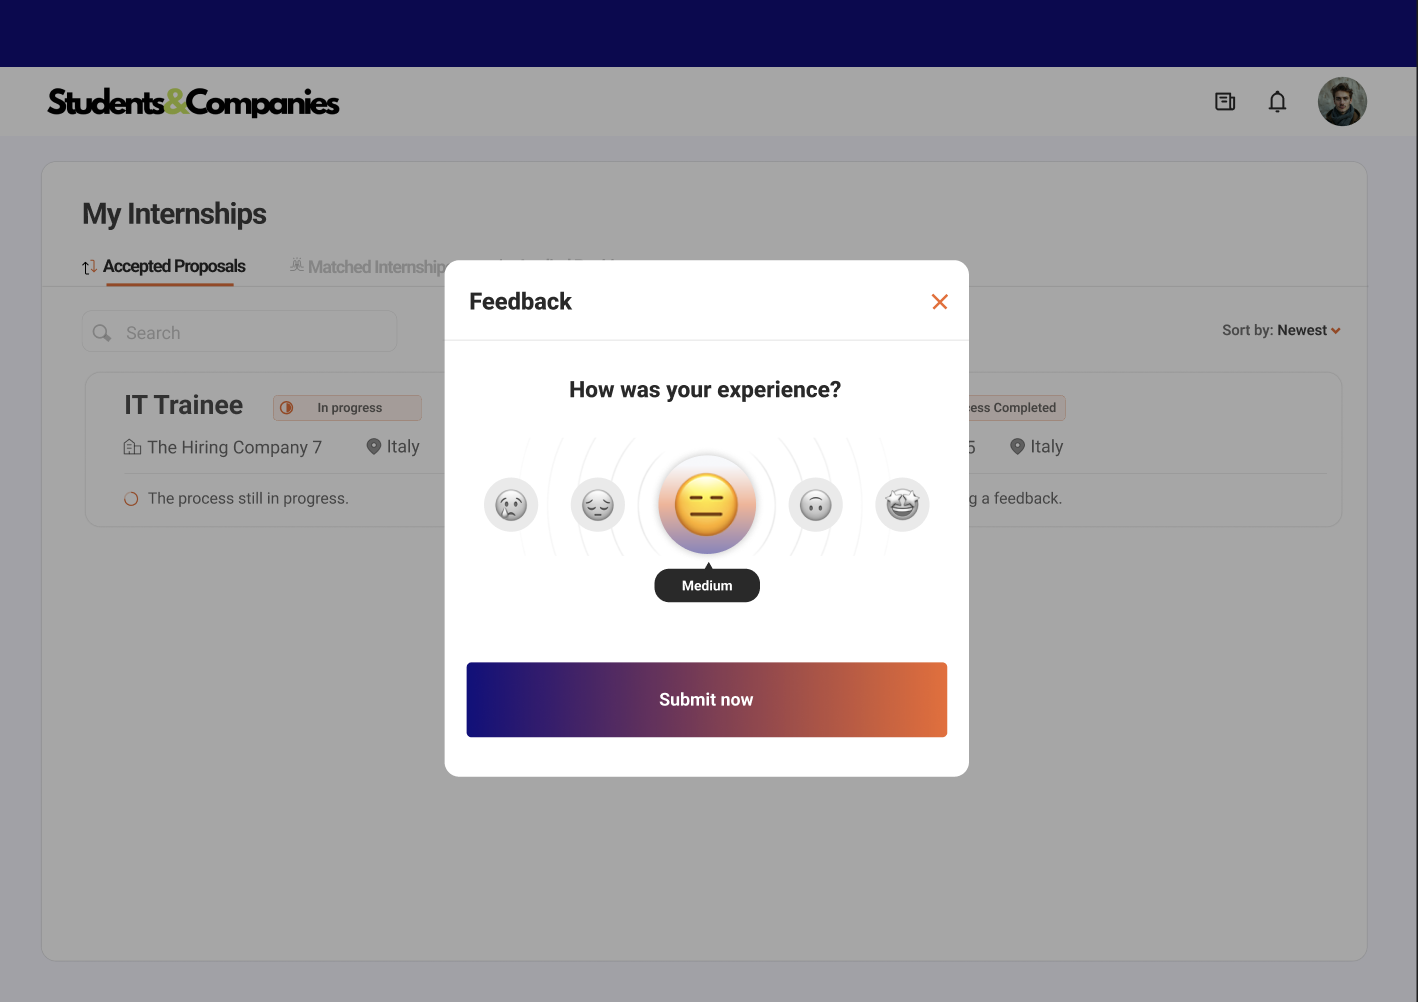
\includegraphics[scale = 0.42]{figures/UserInterfaces/Student/Feedback.png}
    \caption{Student Feedback}
     \centering
\end{figure}

\begin{figure}[H]
    \centering
    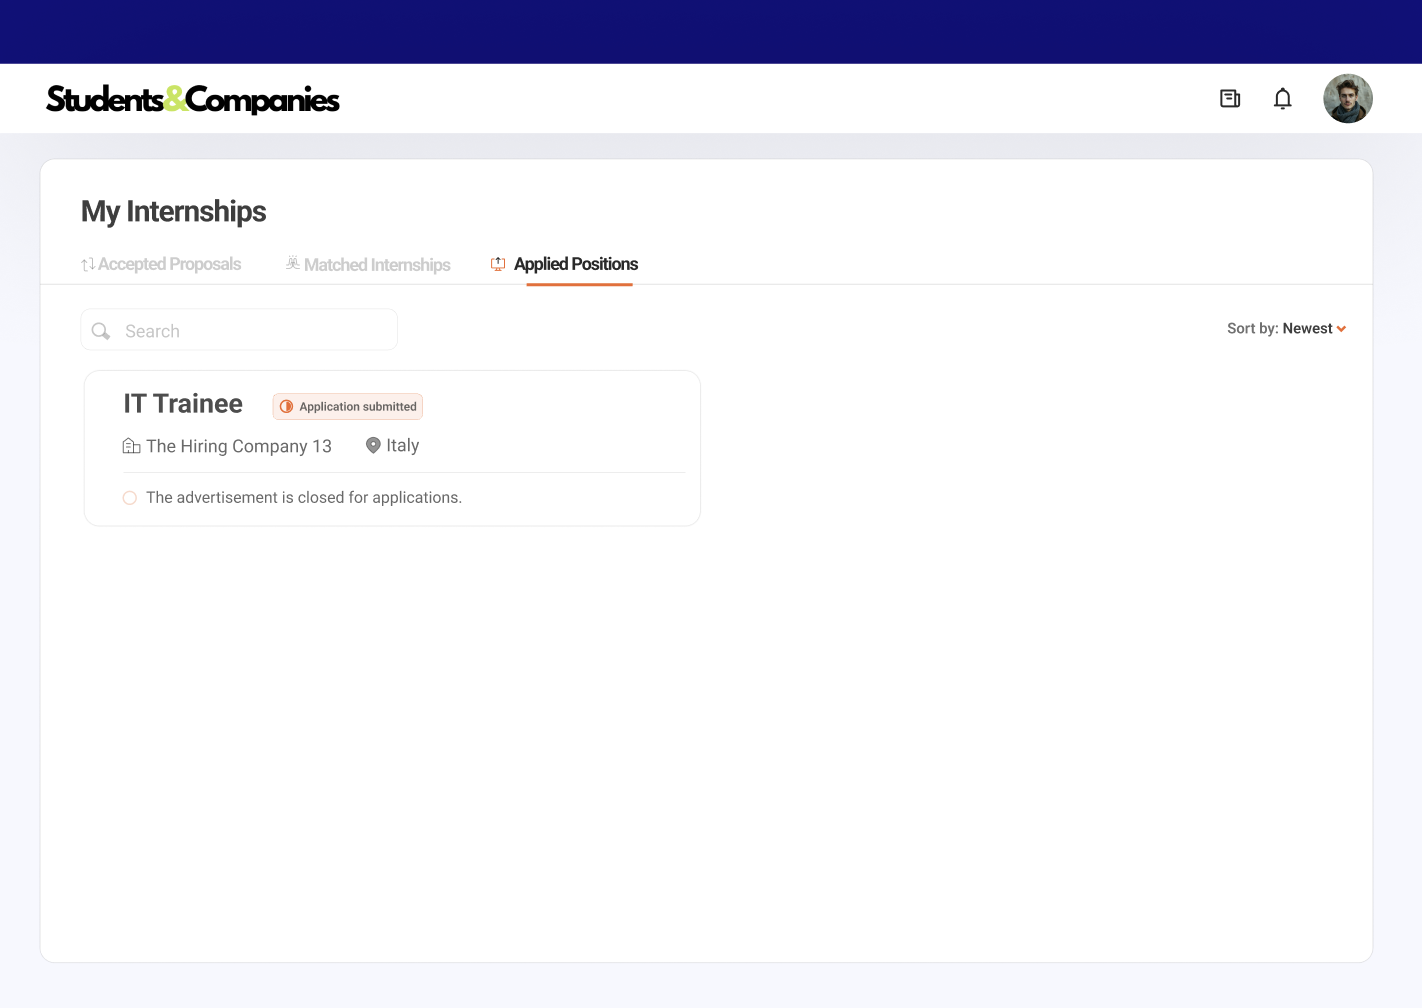
\includegraphics[scale = 0.42]{figures/UserInterfaces/Student/AppliedPositions.png}
    \caption{Student Applied Internships}
     \centering
\end{figure}

\begin{figure}[H]
    \centering
    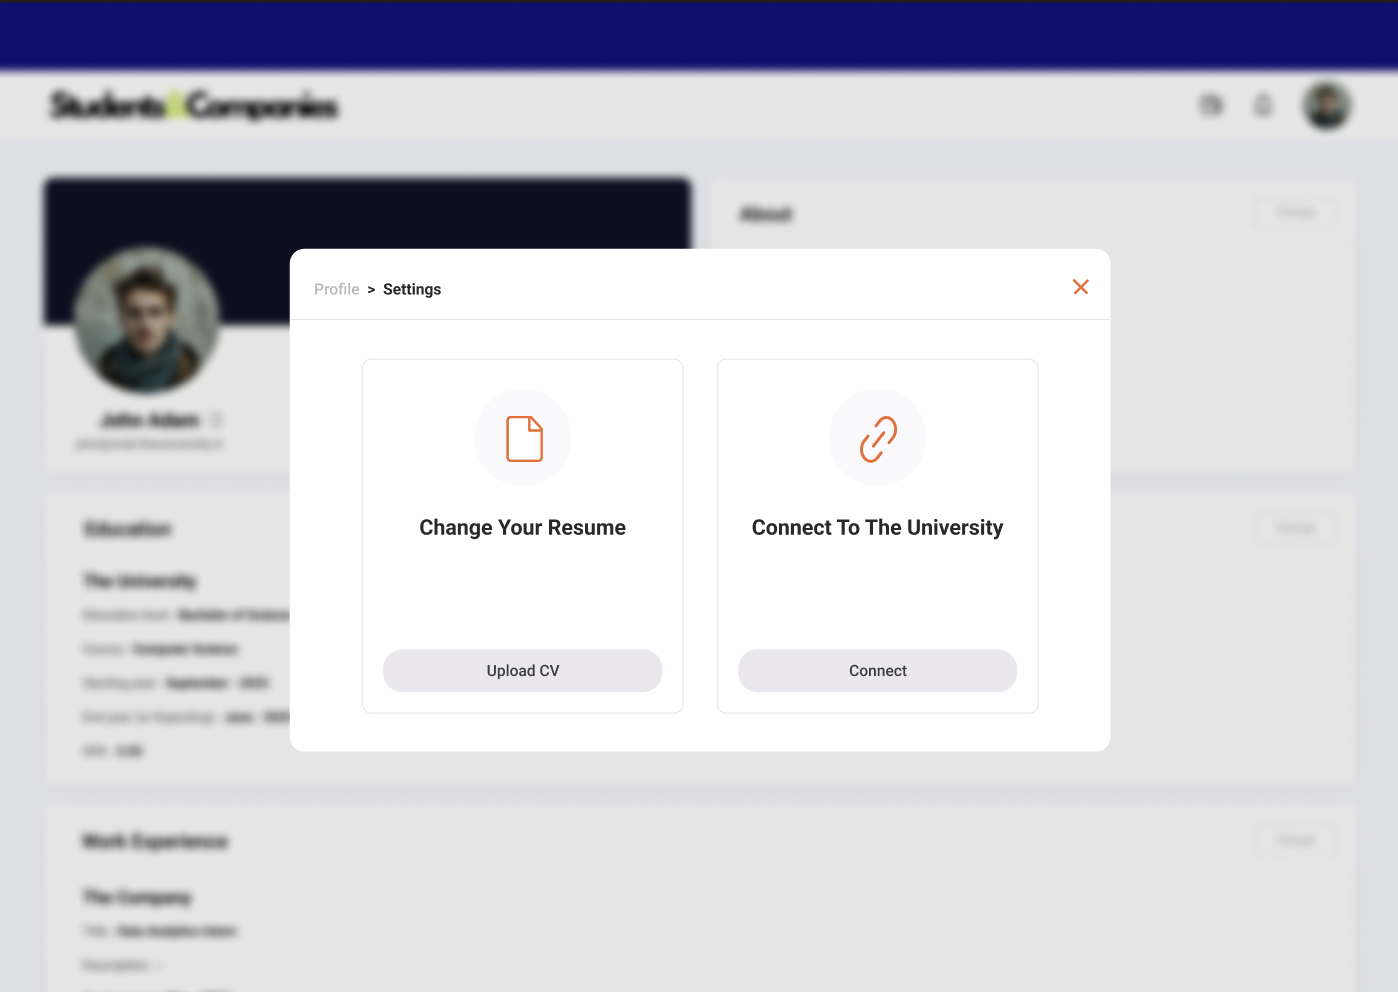
\includegraphics[scale = 0.42]{figures/UserInterfaces/Student/Settings.png}
    \caption{Student Settings}
     \centering
\end{figure}
\begin{figure}[H]
    \centering
    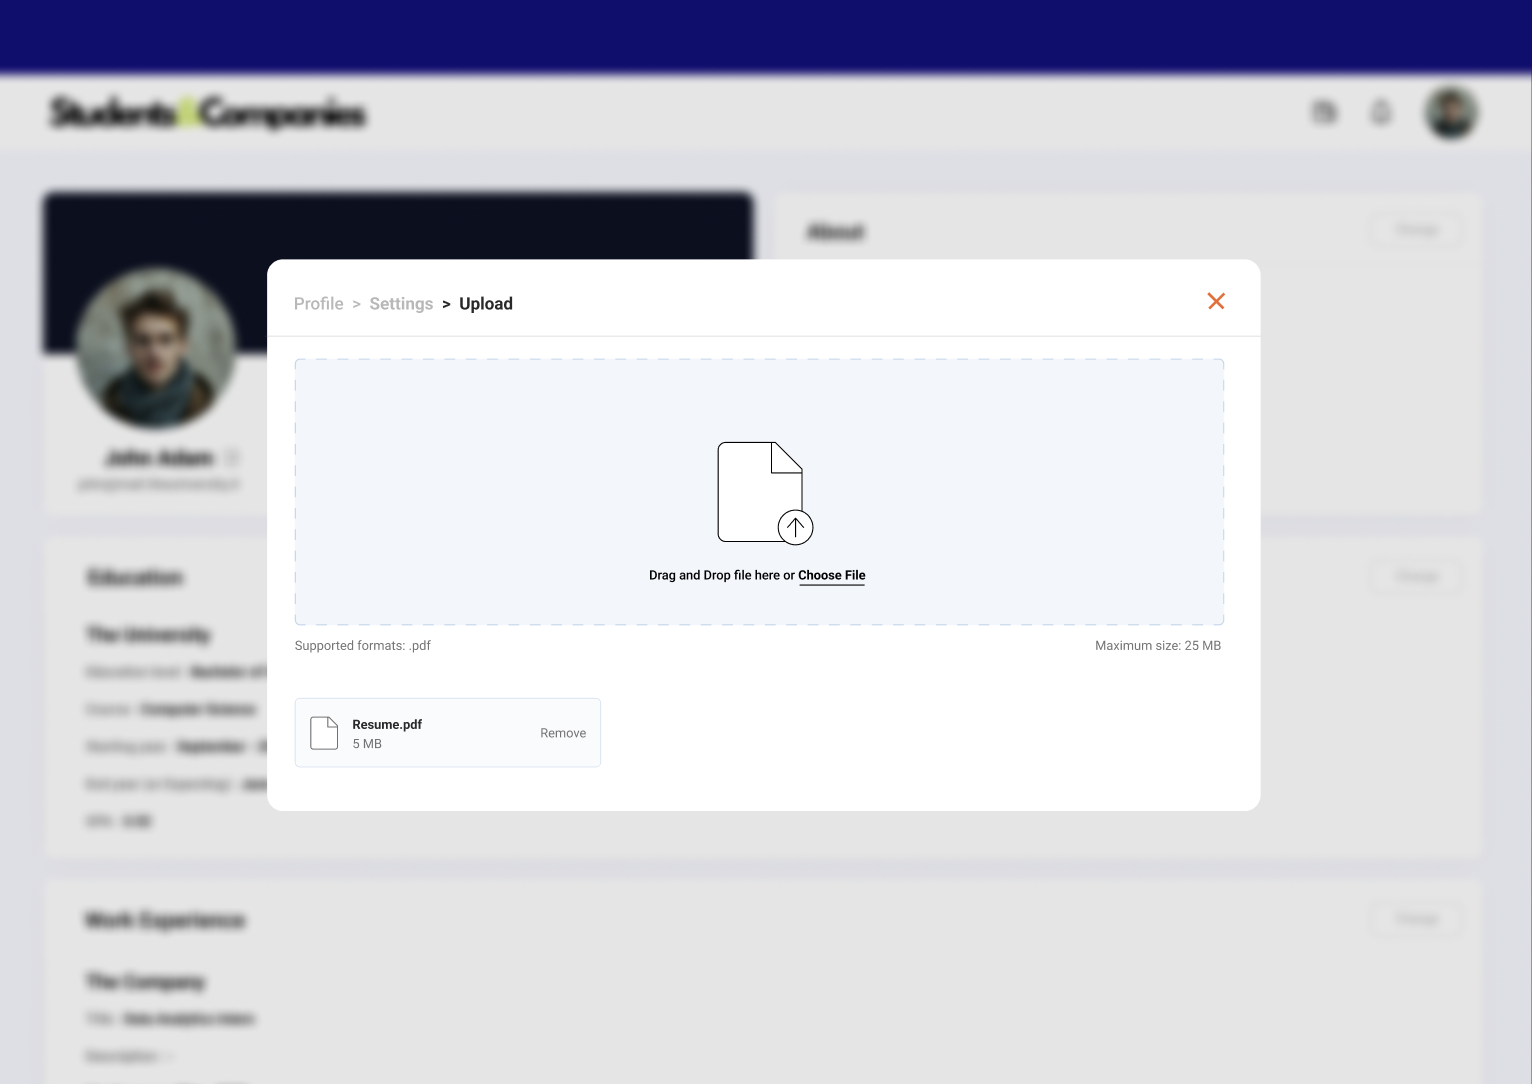
\includegraphics[scale = 0.42]{figures/UserInterfaces/Student/UploadCv.png}
    \caption{Student Update CV}
     \centering
\end{figure}
\begin{figure}[H]
    \centering
    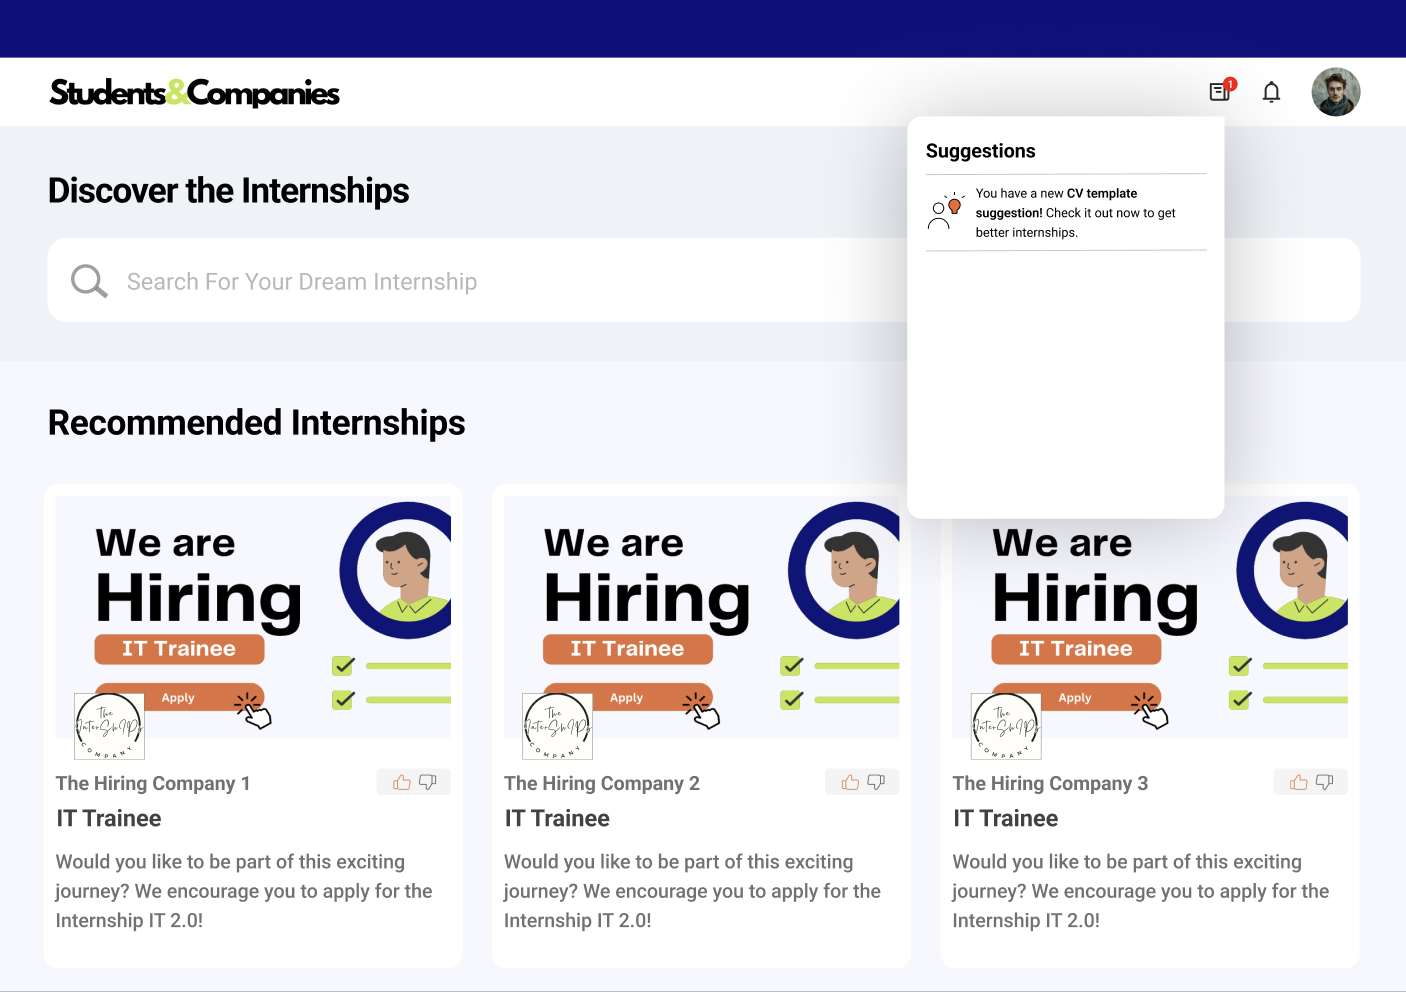
\includegraphics[scale = 0.42]{figures/UserInterfaces/Student/SuggestionNotification.png}
    \caption{Student Suggestions Notification}
     \centering
\end{figure}
\begin{figure}[H]
    \centering
    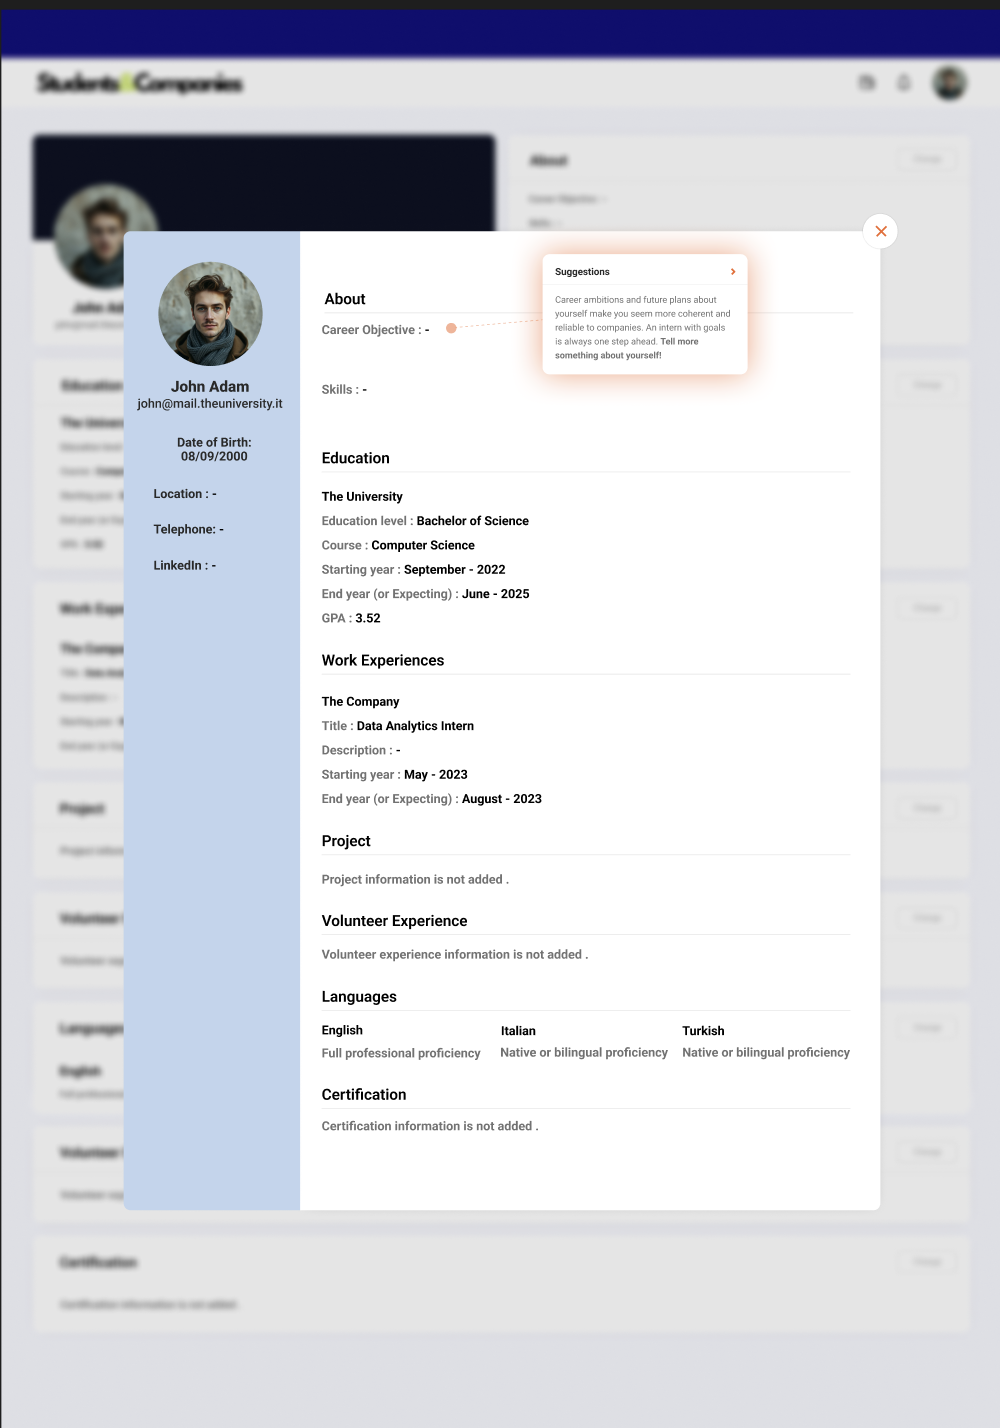
\includegraphics[scale = 0.65]{figures/UserInterfaces/Student/CVSuggestion.png}
    \caption{Student CV Suggestion Template}
     \centering
\end{figure}

\begin{figure}[H]
    \centering
    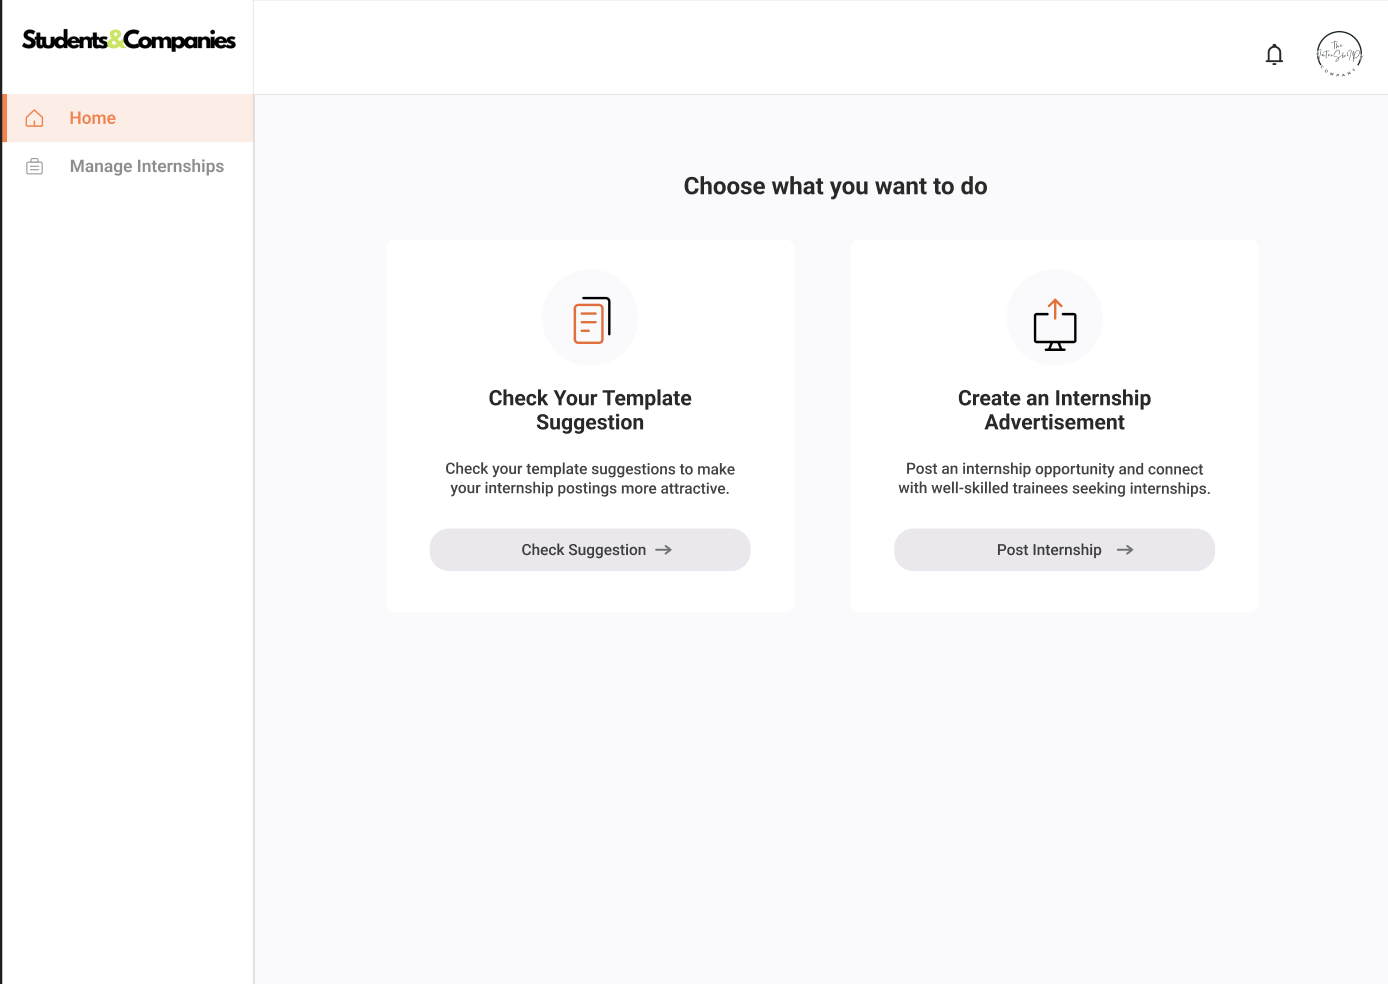
\includegraphics[scale = 0.42]{figures/UserInterfaces/Company/CompanyHome.png}
    \caption{Company Home Page}
     \centering
\end{figure}
\begin{figure}[H]
    \centering
    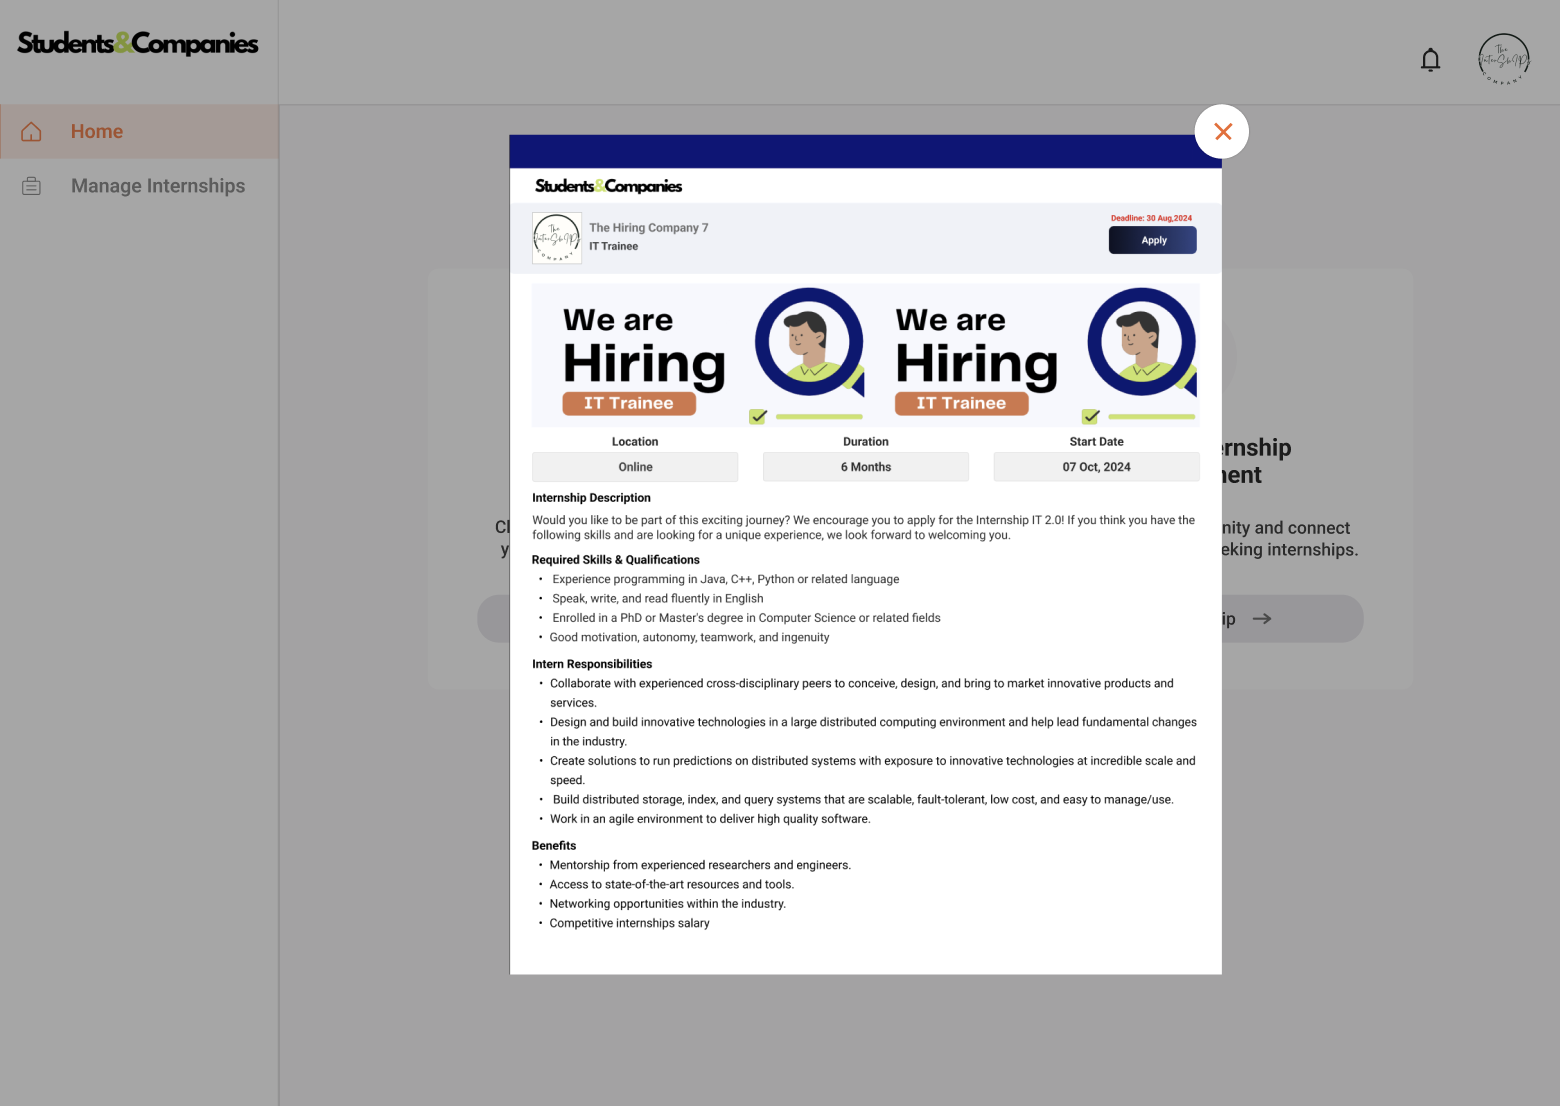
\includegraphics[scale = 0.40]{figures/UserInterfaces/Company/CompanySuggestion.png}
    \caption{Company Advertisement Suggestion Template}
     \centering
\end{figure}
\begin{figure}[H]
    \centering
    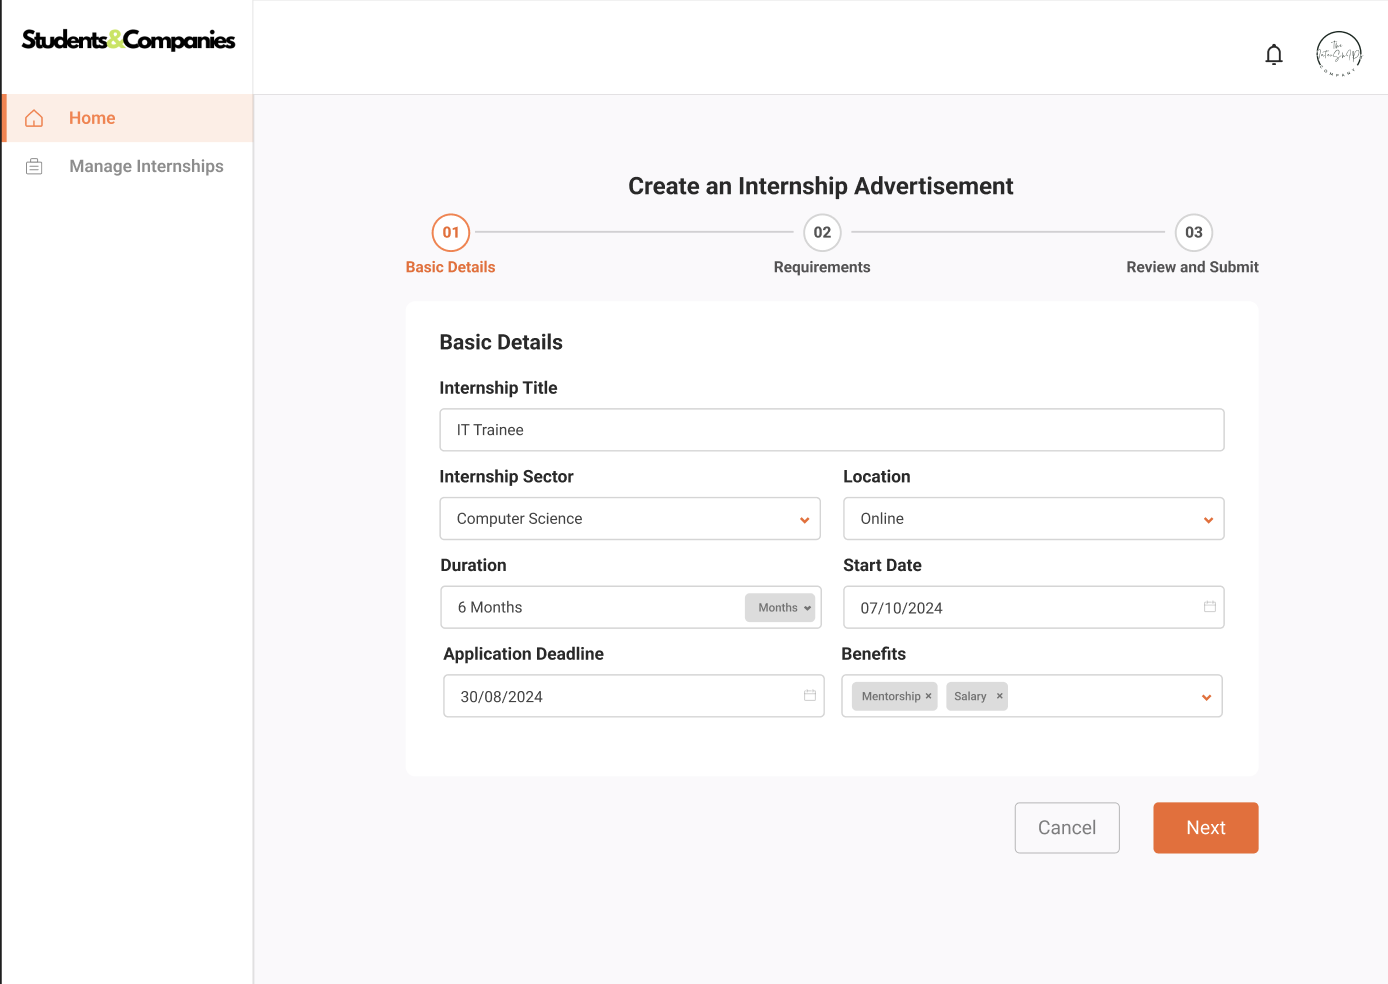
\includegraphics[scale = 0.42]{figures/UserInterfaces/Company/CreateInternship1.png}
    \caption{Create Internship Page 1}
     \centering
\end{figure}
\begin{figure}[H]
    \centering
    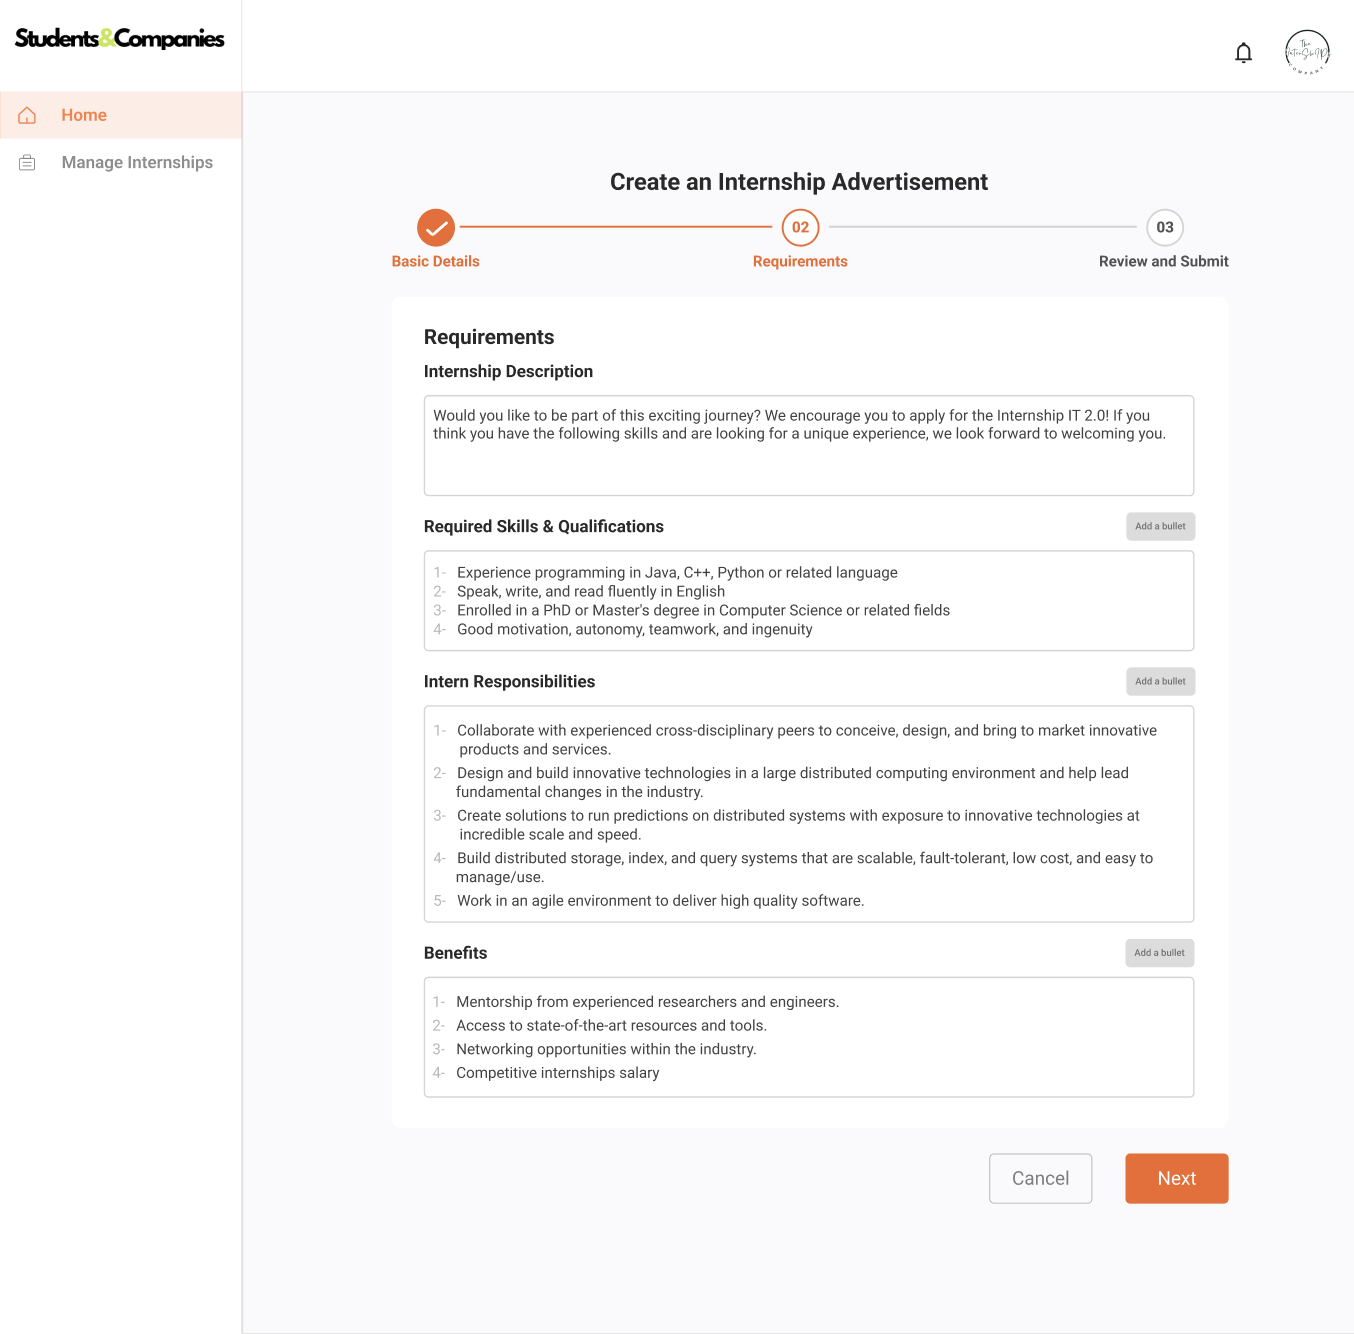
\includegraphics[scale = 0.40]{figures/UserInterfaces/Company/CreateInternship2.png}
    \caption{Create Internship Page 2}
     \centering
\end{figure}
\begin{figure}[H]
    \centering
    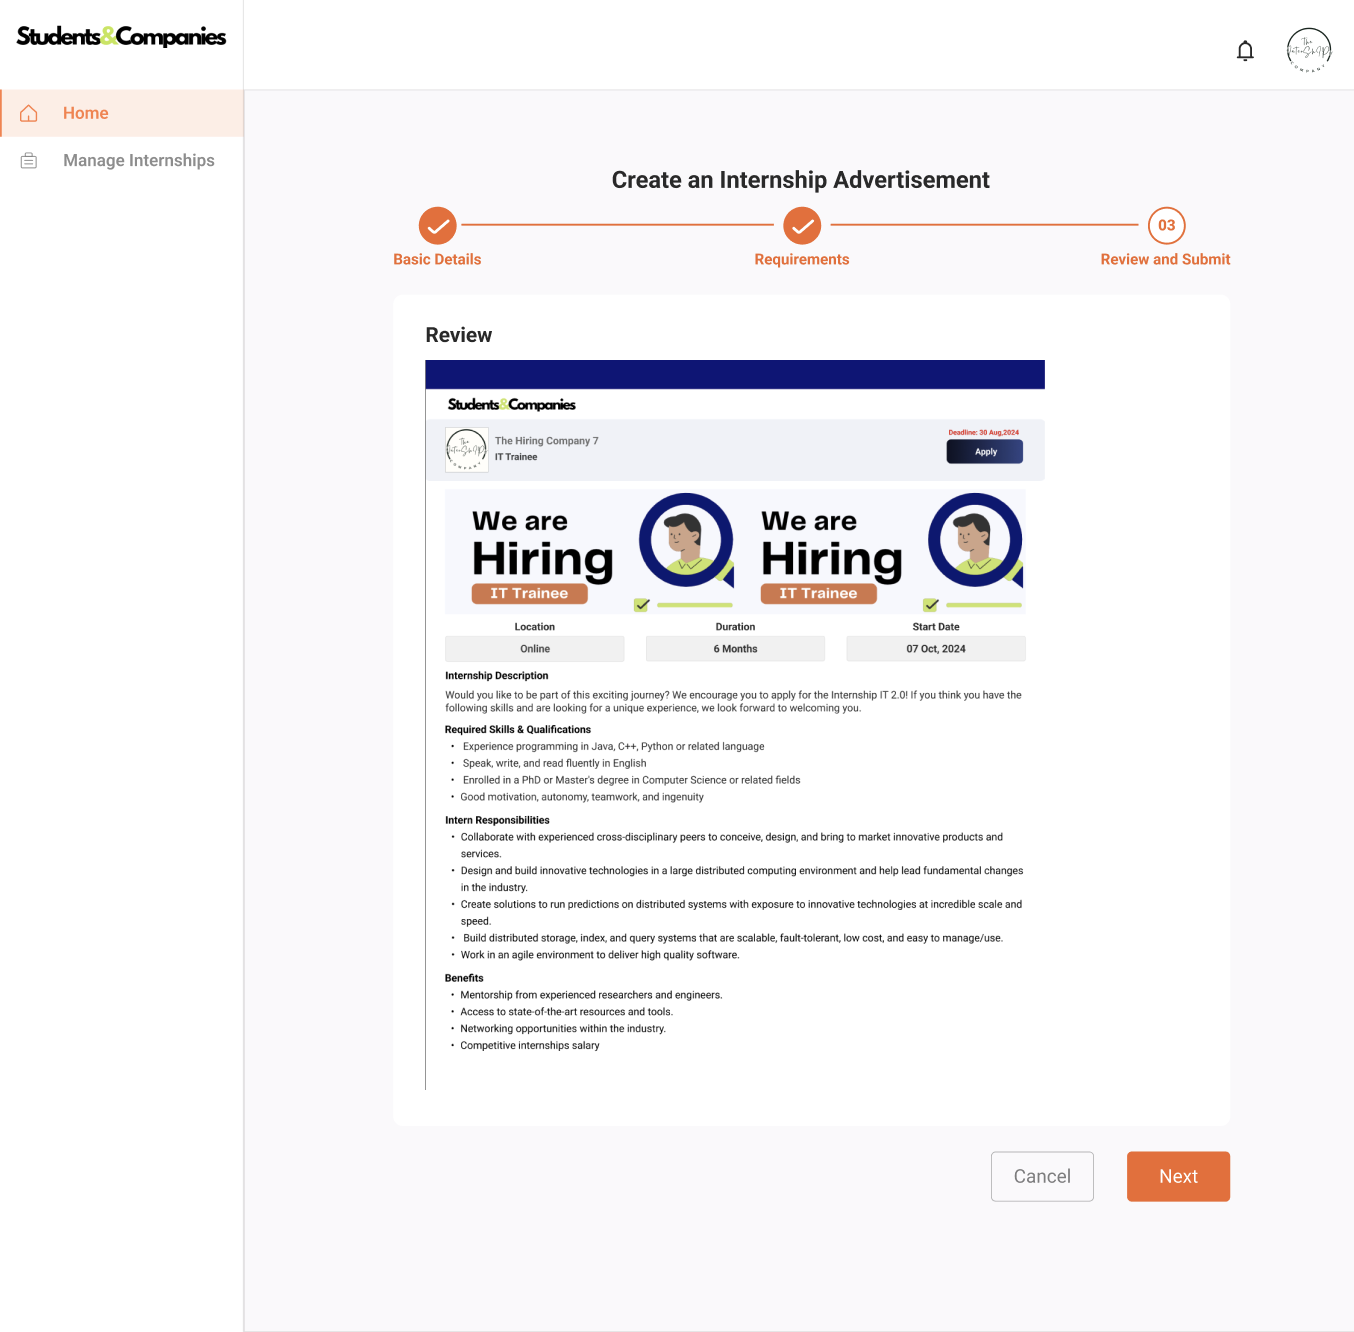
\includegraphics[scale = 0.40]{figures/UserInterfaces/Company/CreateInternship3.png}
    \caption{Create Internship Page 3}
     \centering
\end{figure}
\begin{figure}[H]
    \centering
    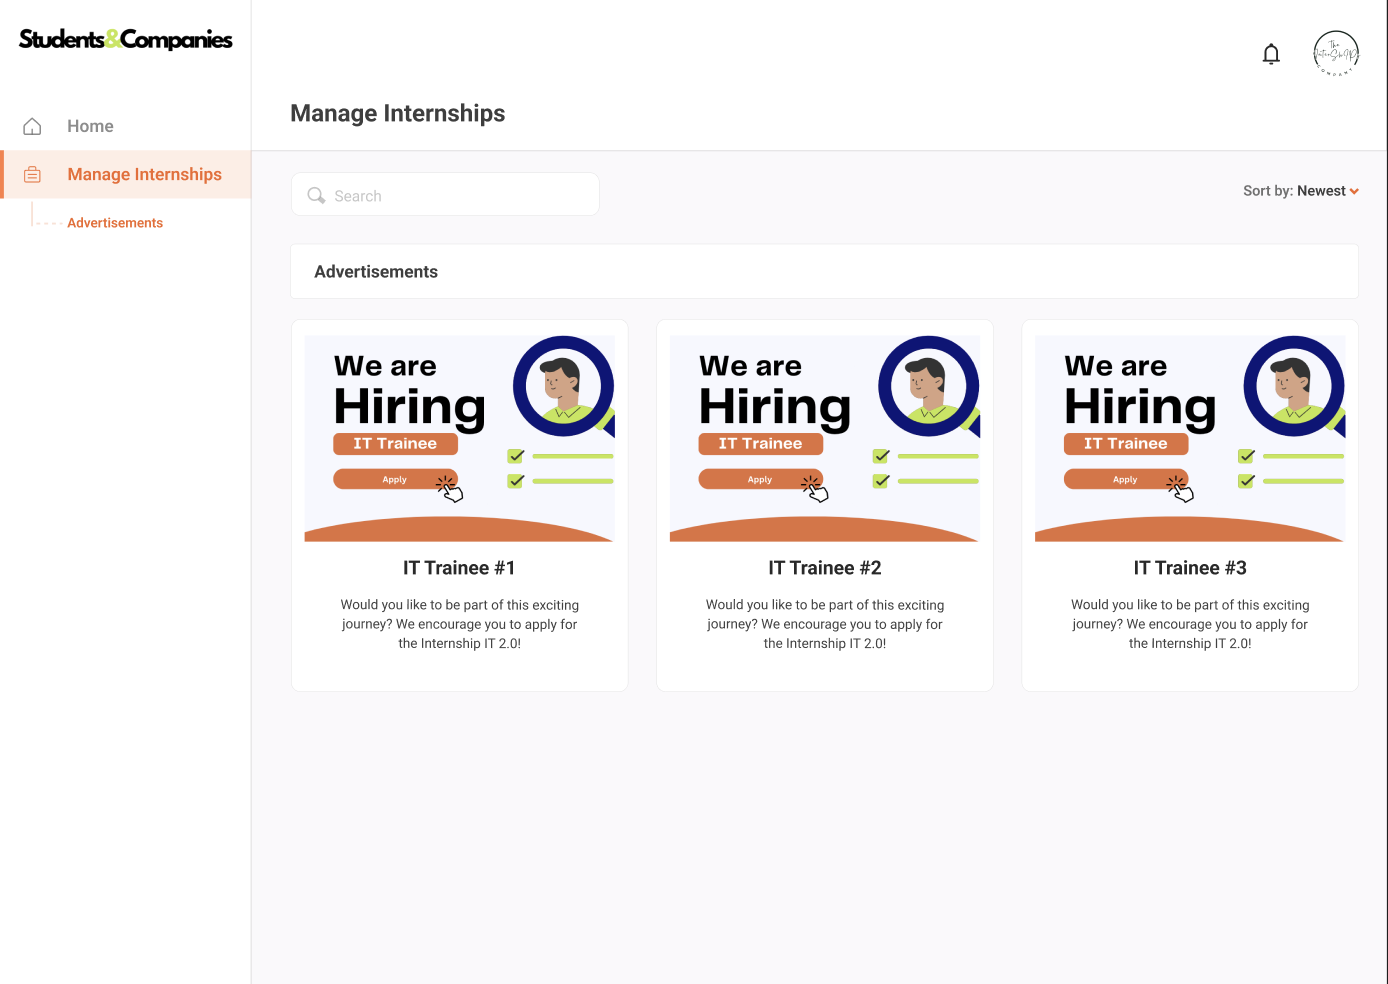
\includegraphics[scale = 0.40]{figures/UserInterfaces/Company/ManageInternships.png}
    \caption{Manage Internships Page}
     \centering
\end{figure}
\begin{figure}[H]
    \centering
    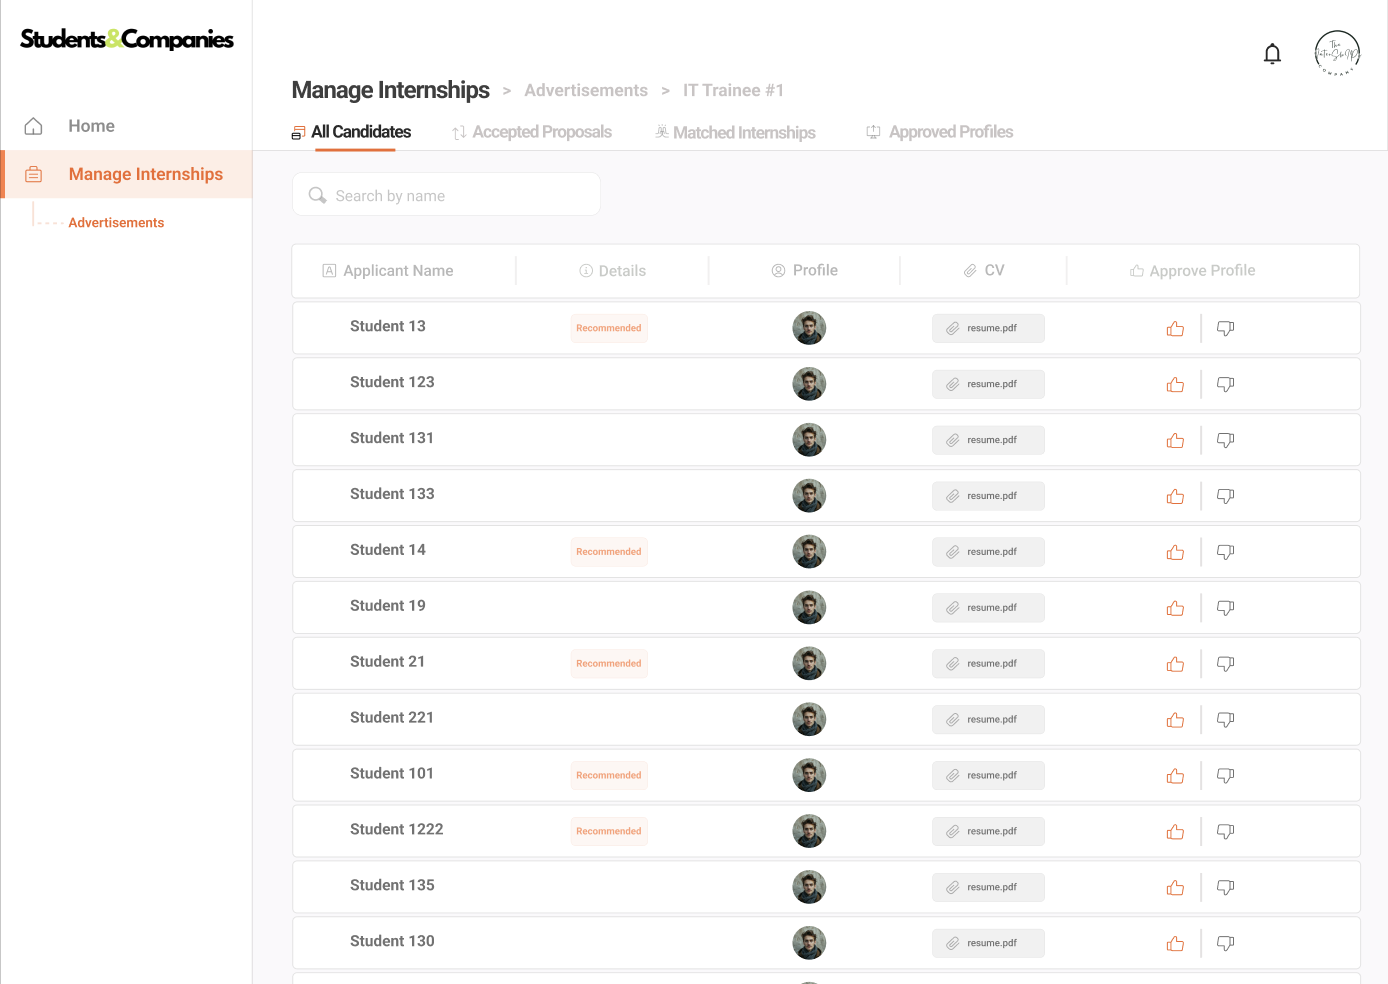
\includegraphics[scale = 0.42]{figures/UserInterfaces/Company/AllCandidatesCompany.png}
    \caption{All Candidates Page}
     \centering
\end{figure}
\begin{figure}[H]
    \centering
    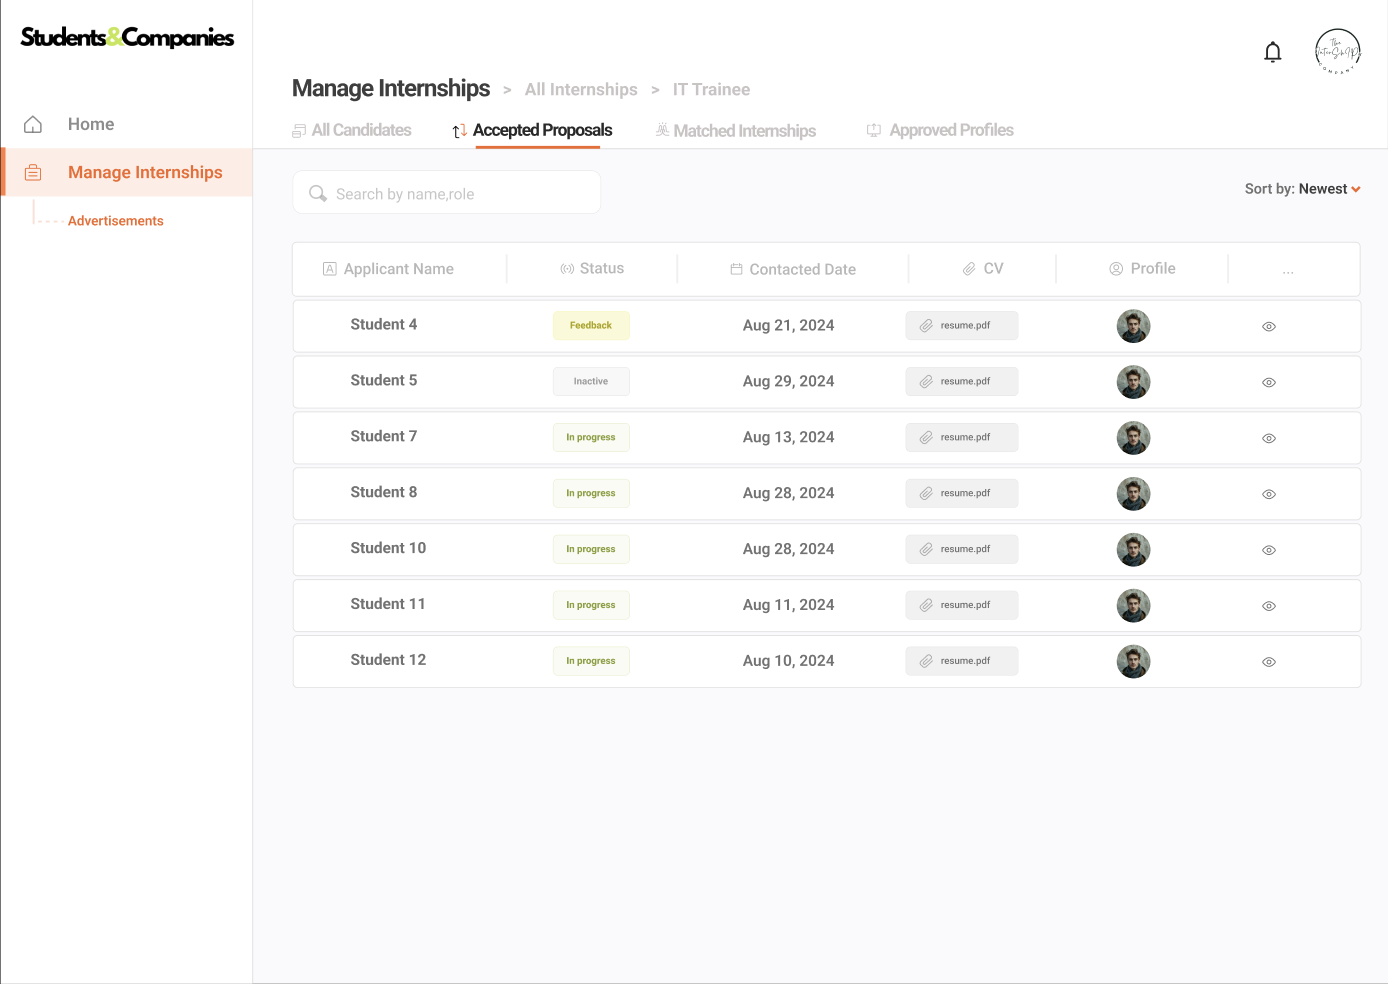
\includegraphics[scale = 0.42]{figures/UserInterfaces/Company/AcceptedProposalCompany.png}
    \caption{Company Accepted Proposals Page}
     \centering
\end{figure}
\begin{figure}[H]
    \centering
    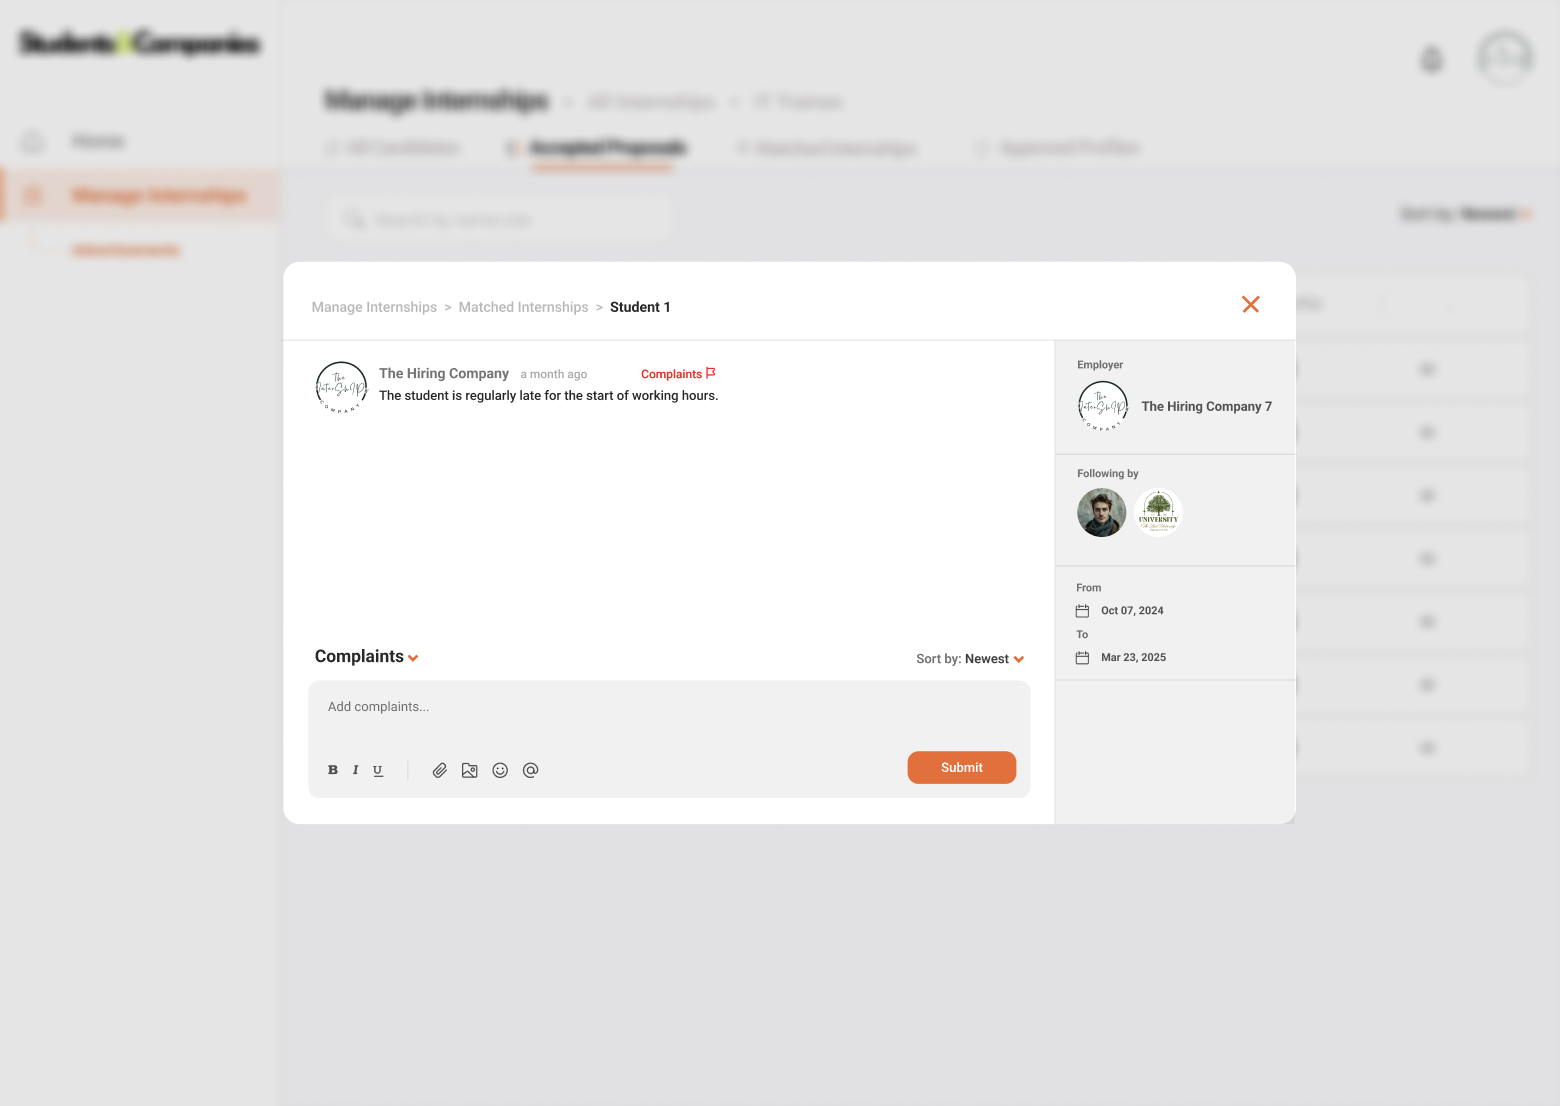
\includegraphics[scale = 0.42]{figures/UserInterfaces/Company/CompanyComplaints.png}
    \caption{Company Ongoing Internship Complaints Page}
     \centering
\end{figure}
\begin{figure}[H]
    \centering
    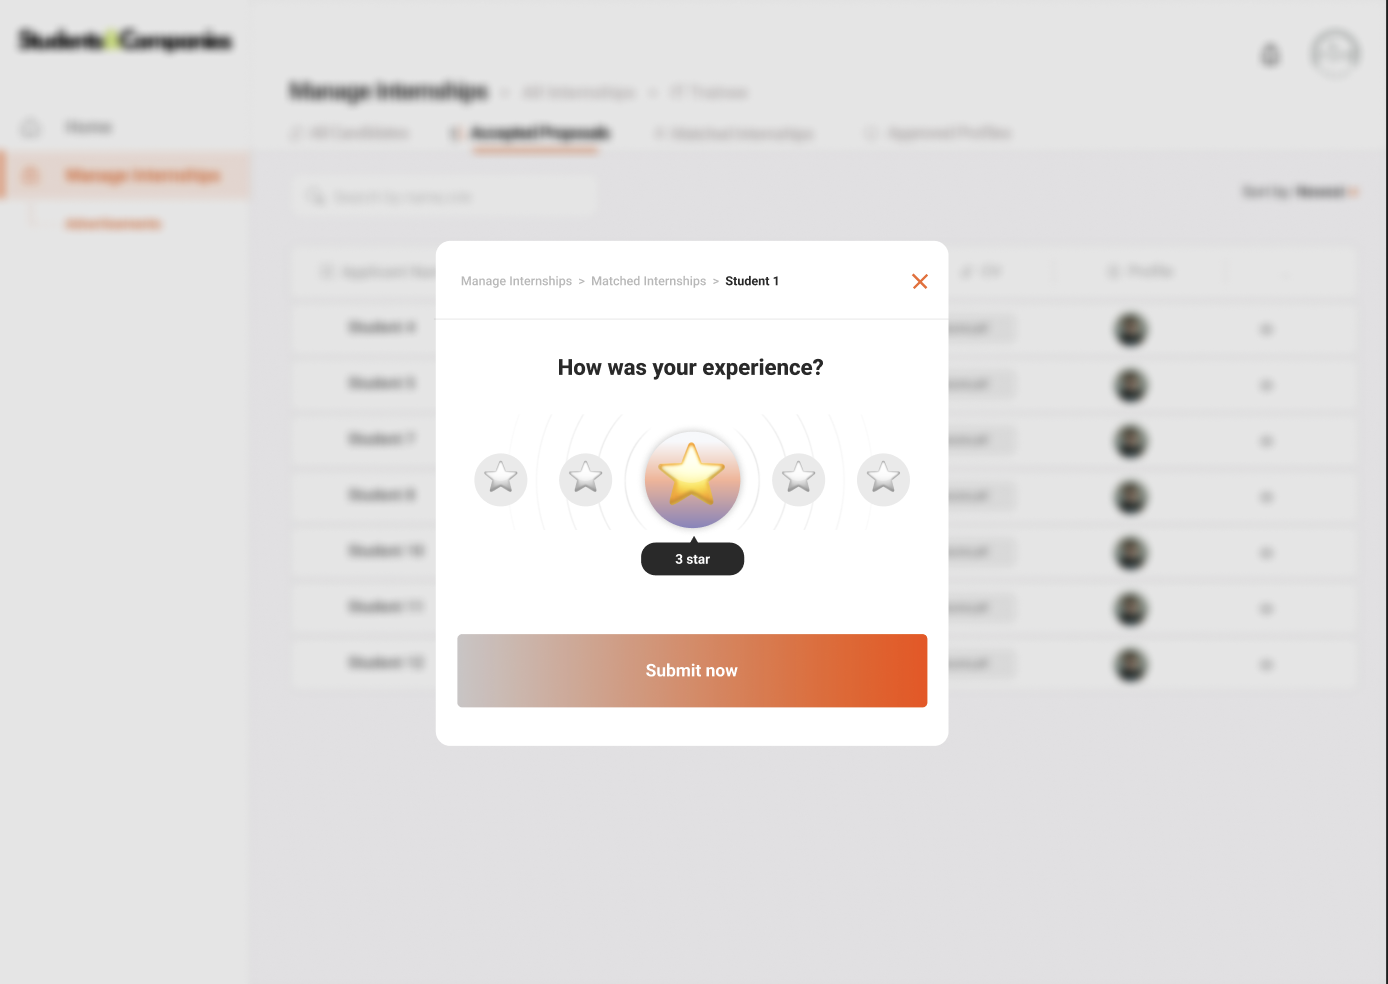
\includegraphics[scale = 0.42]{figures/UserInterfaces/Company/FeedbackCompany.png}
    \caption{Feedback}
     \centering
\end{figure}
\begin{figure}[H]
    \centering
    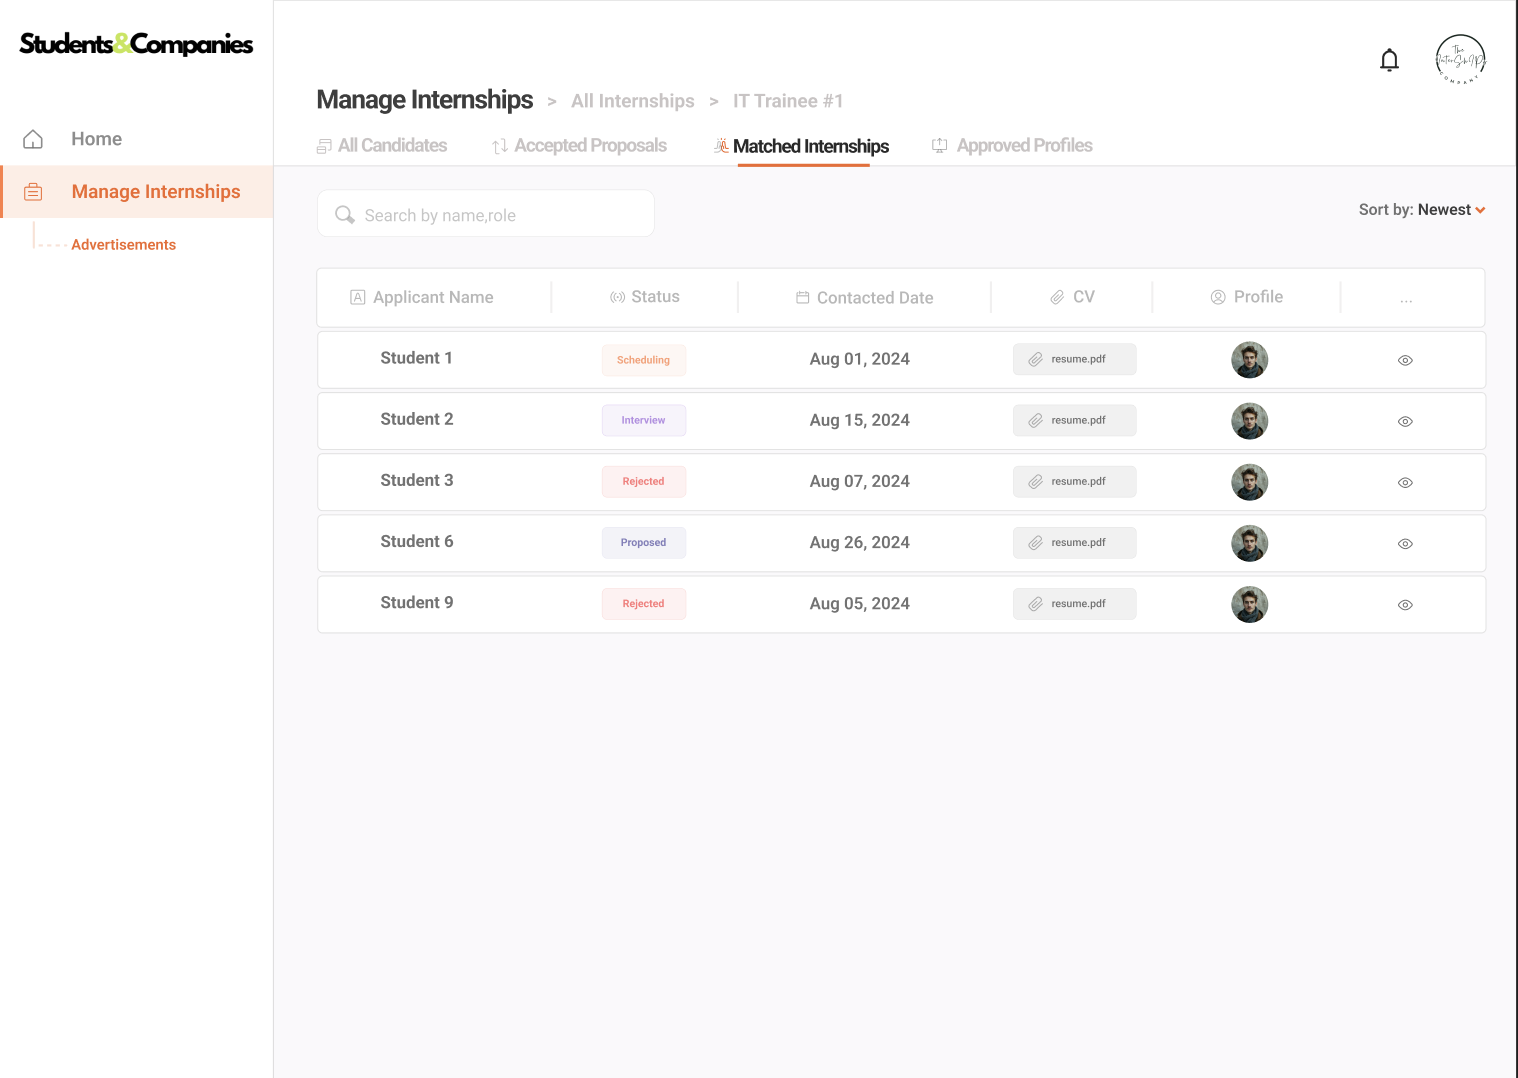
\includegraphics[scale = 0.42]{figures/UserInterfaces/Company/MatchedCompany.png}
    \caption{Company Matched Internships Page}
     \centering
\end{figure}
\begin{figure}[H]
    \centering
    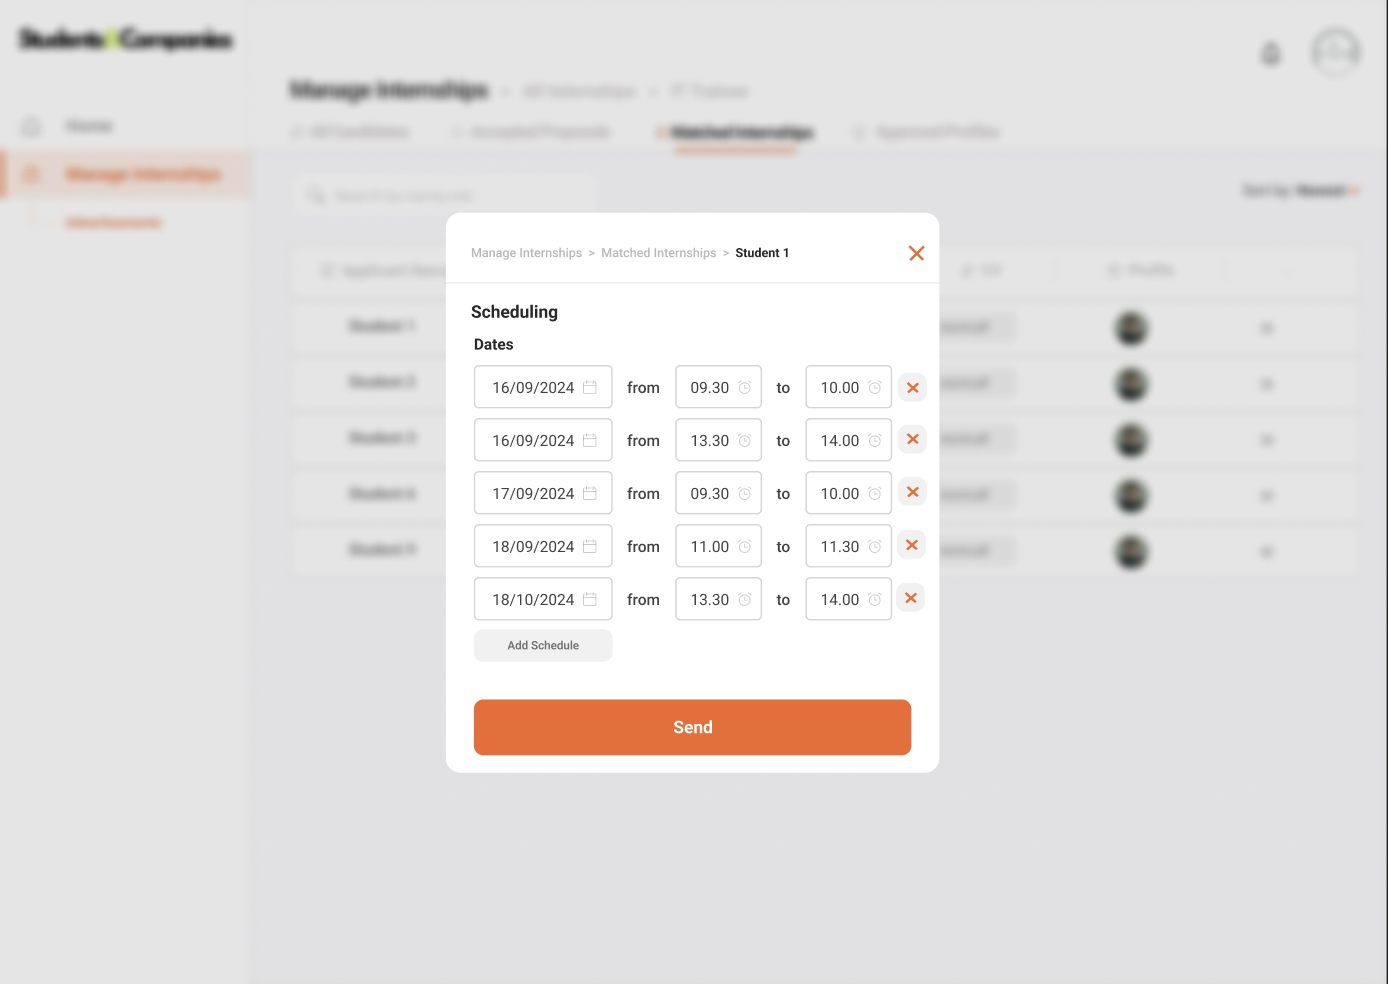
\includegraphics[scale = 0.42]{figures/UserInterfaces/Company/Scheduling.png}
    \caption{Company Interview Scheduling}
     \centering
\end{figure}
\begin{figure}[H]
    \centering
    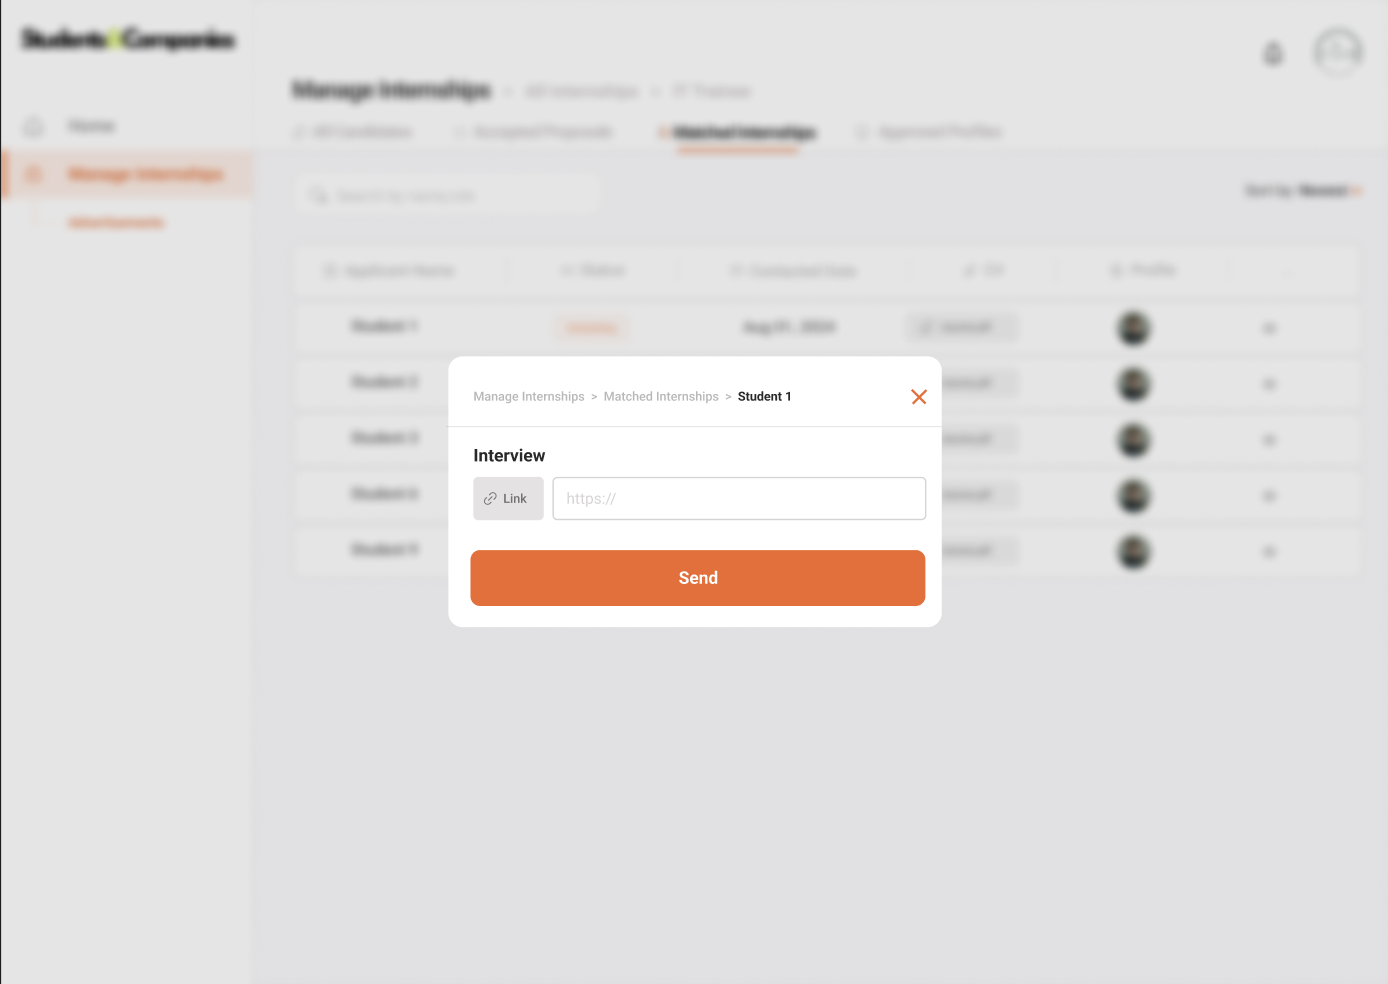
\includegraphics[scale = 0.42]{figures/UserInterfaces/Company/InterviewLink.png}
    \caption{Interview Link}
     \centering
\end{figure}
\begin{figure}[H]
    \centering
    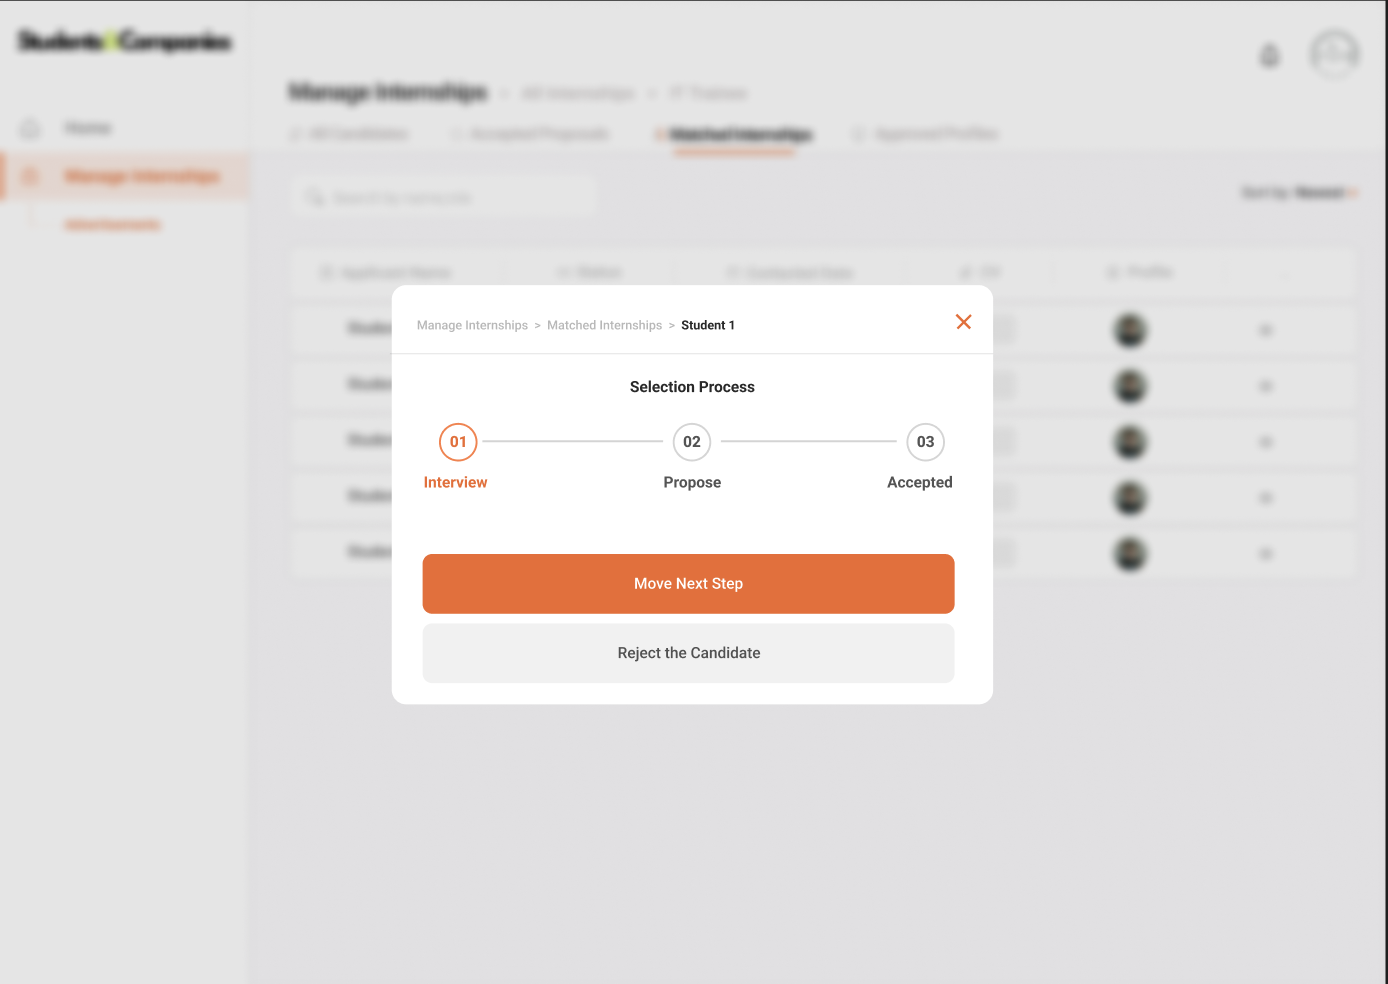
\includegraphics[scale = 0.42]{figures/UserInterfaces/Company/SelectionProcess.png}
    \caption{Student Selection Process Pop-Up}
     \centering
\end{figure}
\begin{figure}[H]
    \centering
    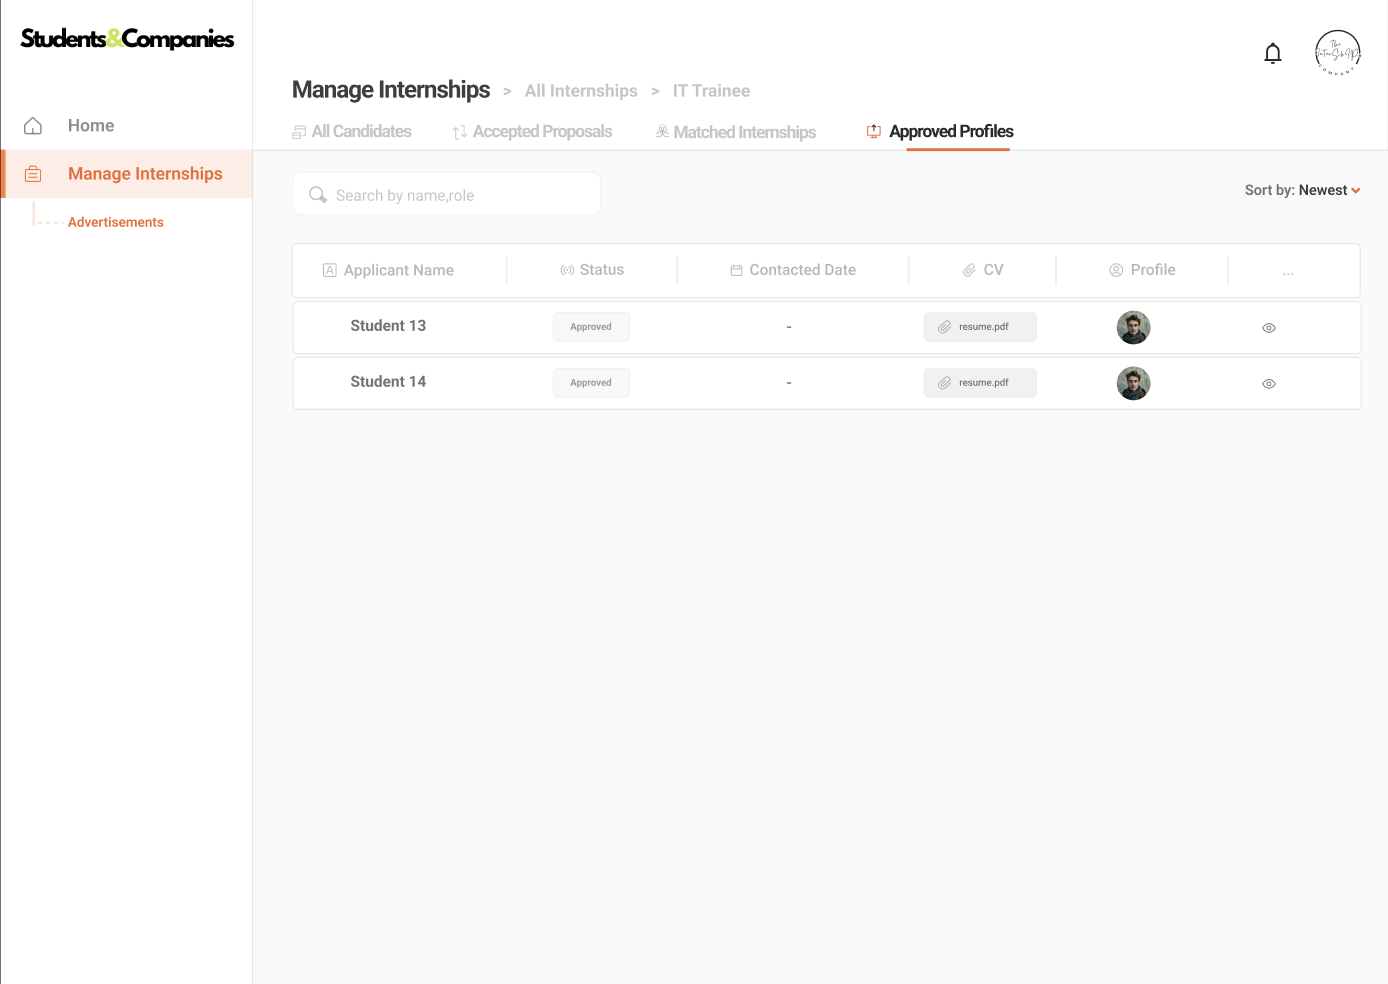
\includegraphics[scale = 0.42]{figures/UserInterfaces/Company/ApprovedProfiles.png}
    \caption{Company Approved Profiles Page}
     \centering
\end{figure}
\begin{figure}[H]
    \centering
    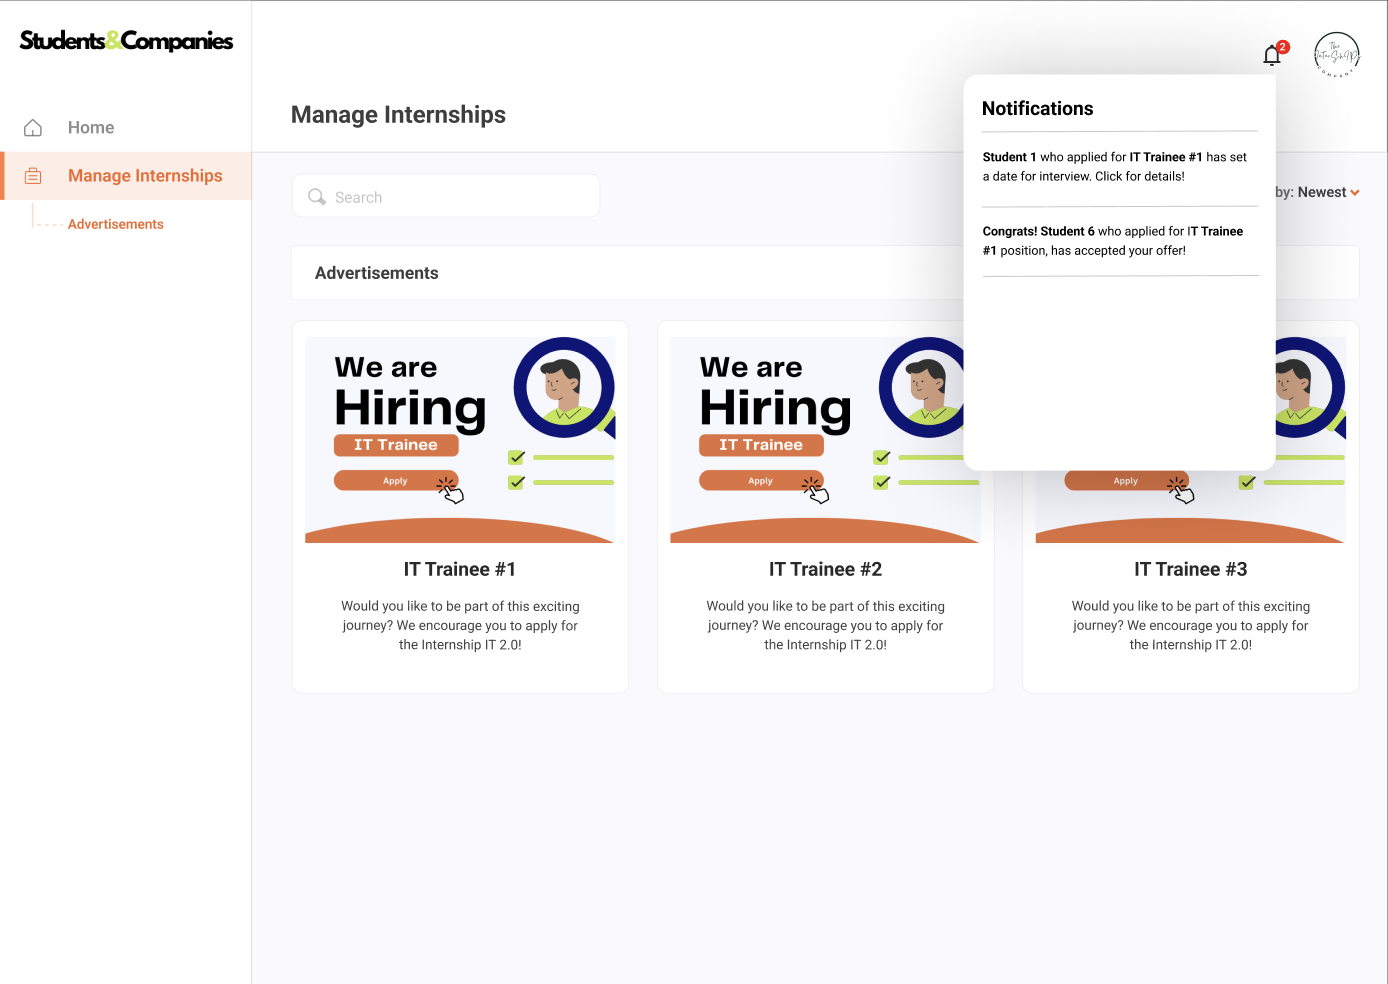
\includegraphics[scale = 0.42]{figures/UserInterfaces/Company/NotificationsCompany.png}
    \caption{Company Notifications}
     \centering
\end{figure}
\begin{figure}[H]
    \centering
    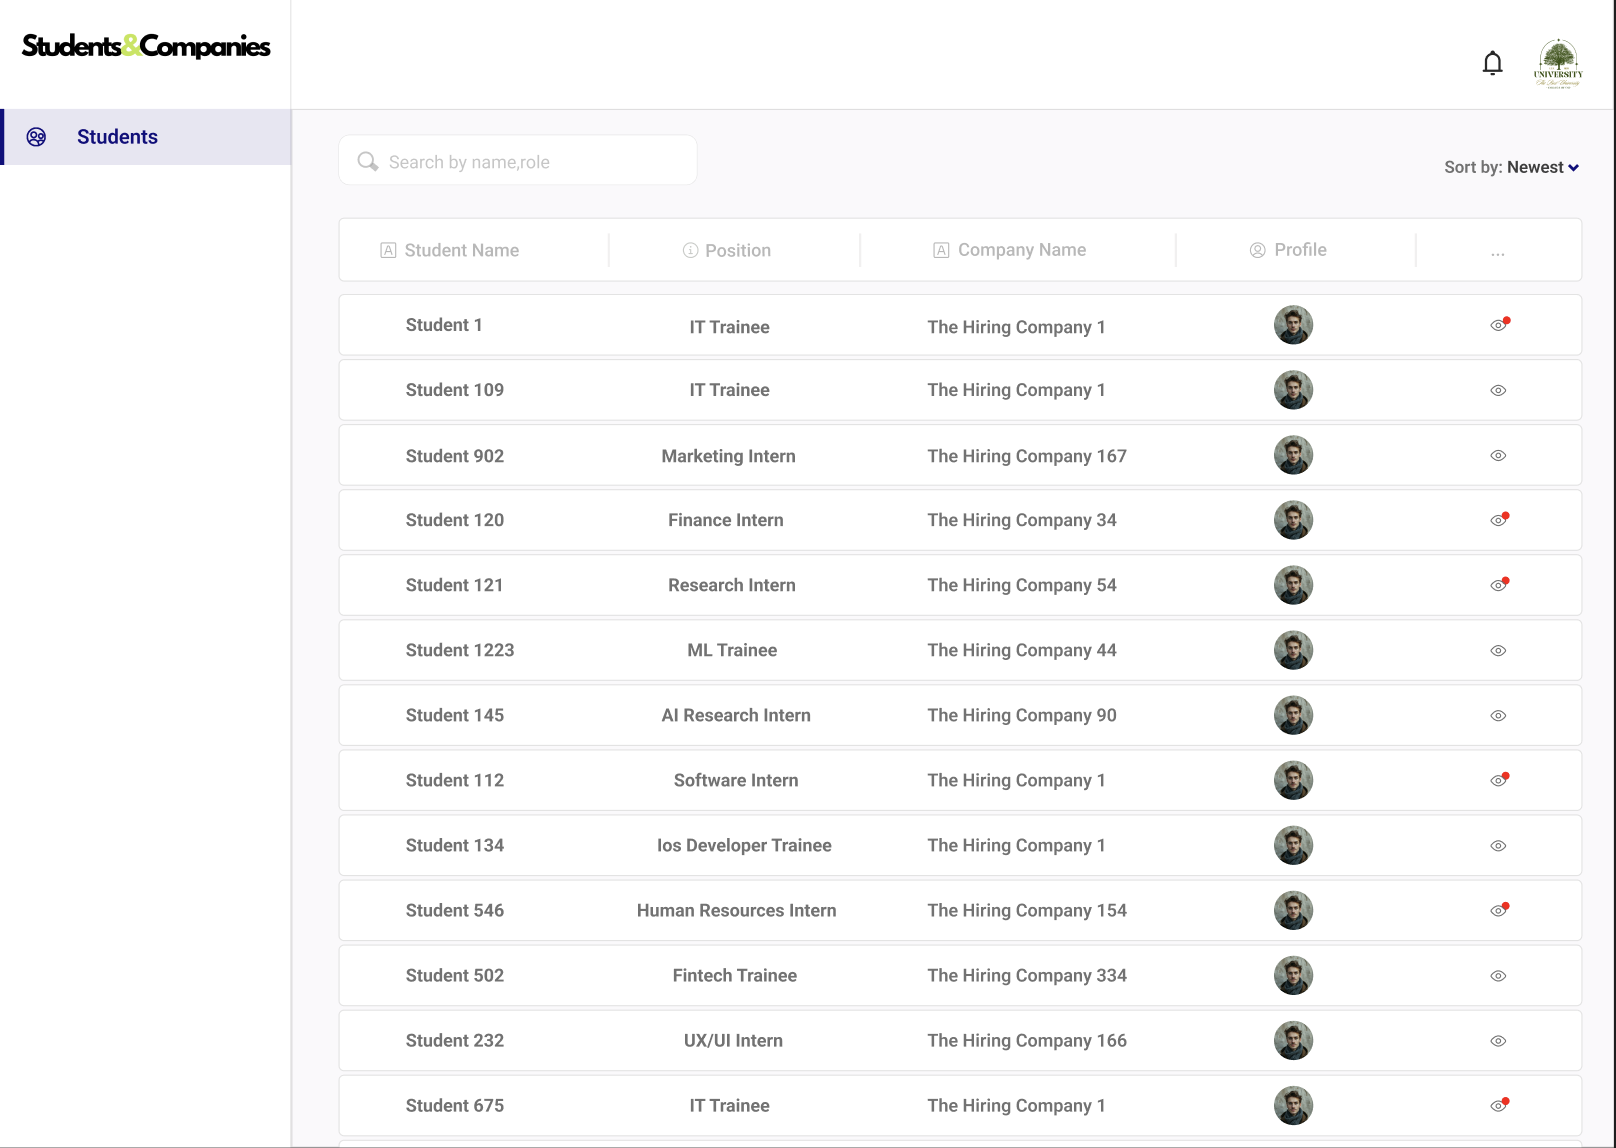
\includegraphics[scale = 0.40]{figures/UserInterfaces/University/UniversityHomePage.png}
    \caption{University Home Page}
     \centering
\end{figure}
\begin{figure}[H]
    \centering
    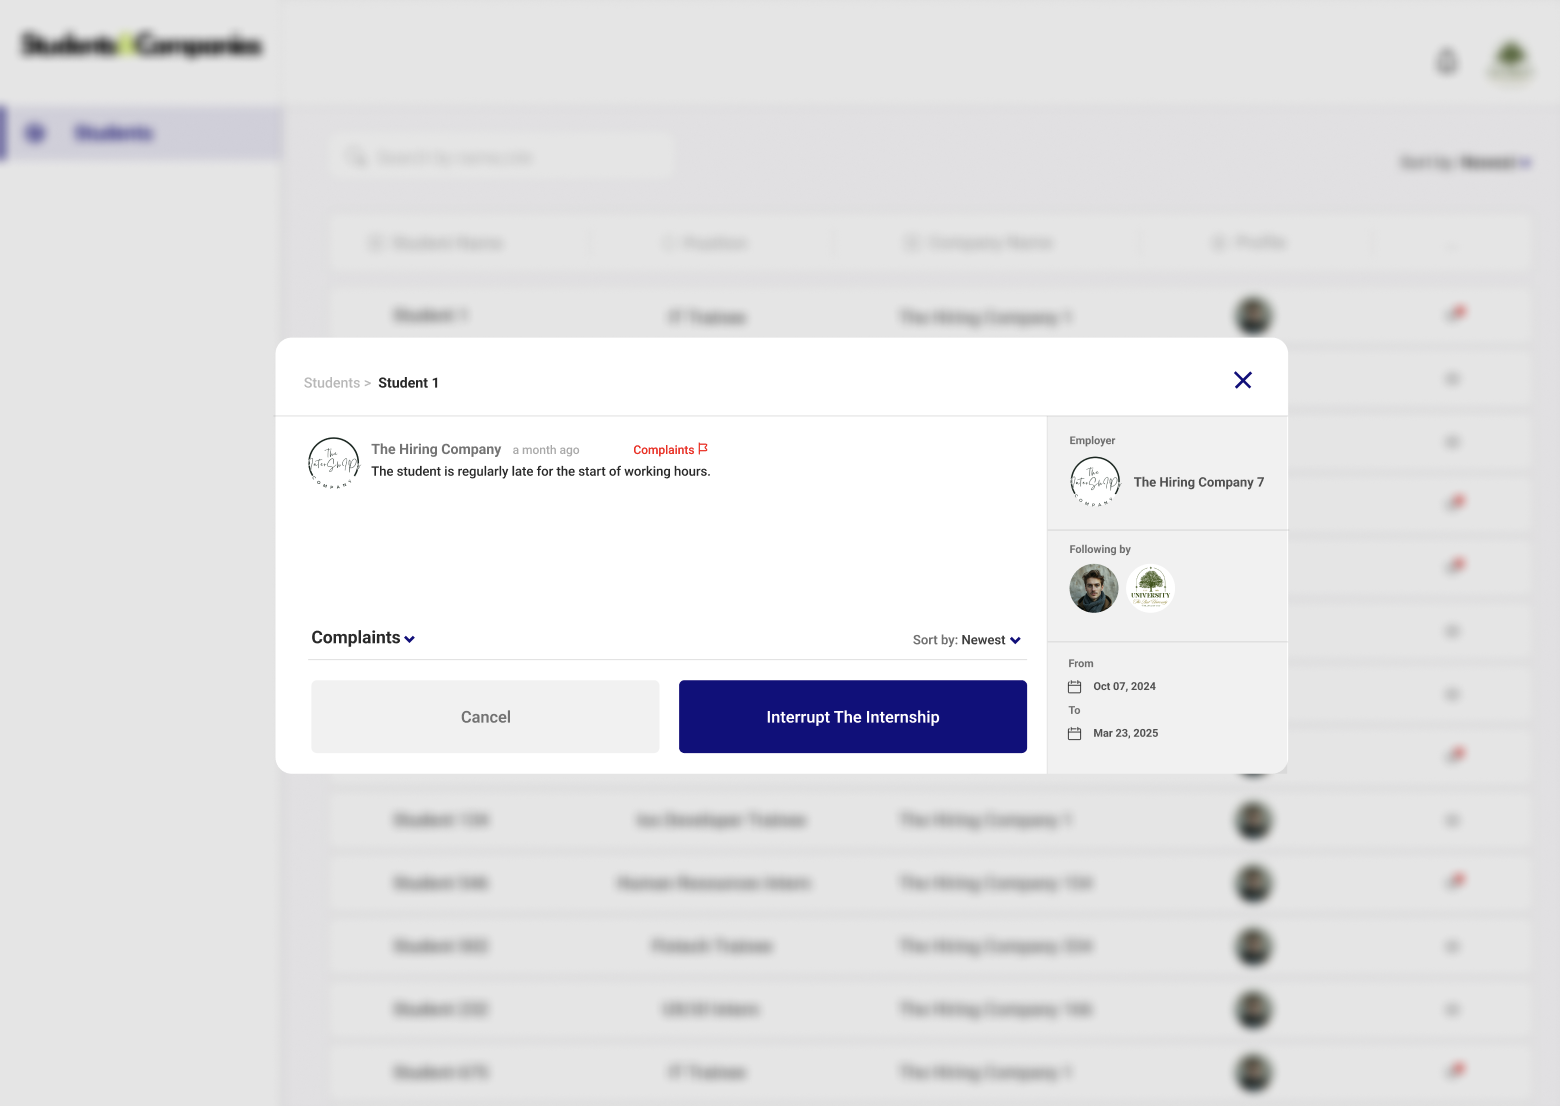
\includegraphics[scale = 0.40]{figures/UserInterfaces/University/InterruptPage.png}
    \caption{University Interrupt Page}
     \centering
\end{figure}
\begin{figure}[H]
    \centering
    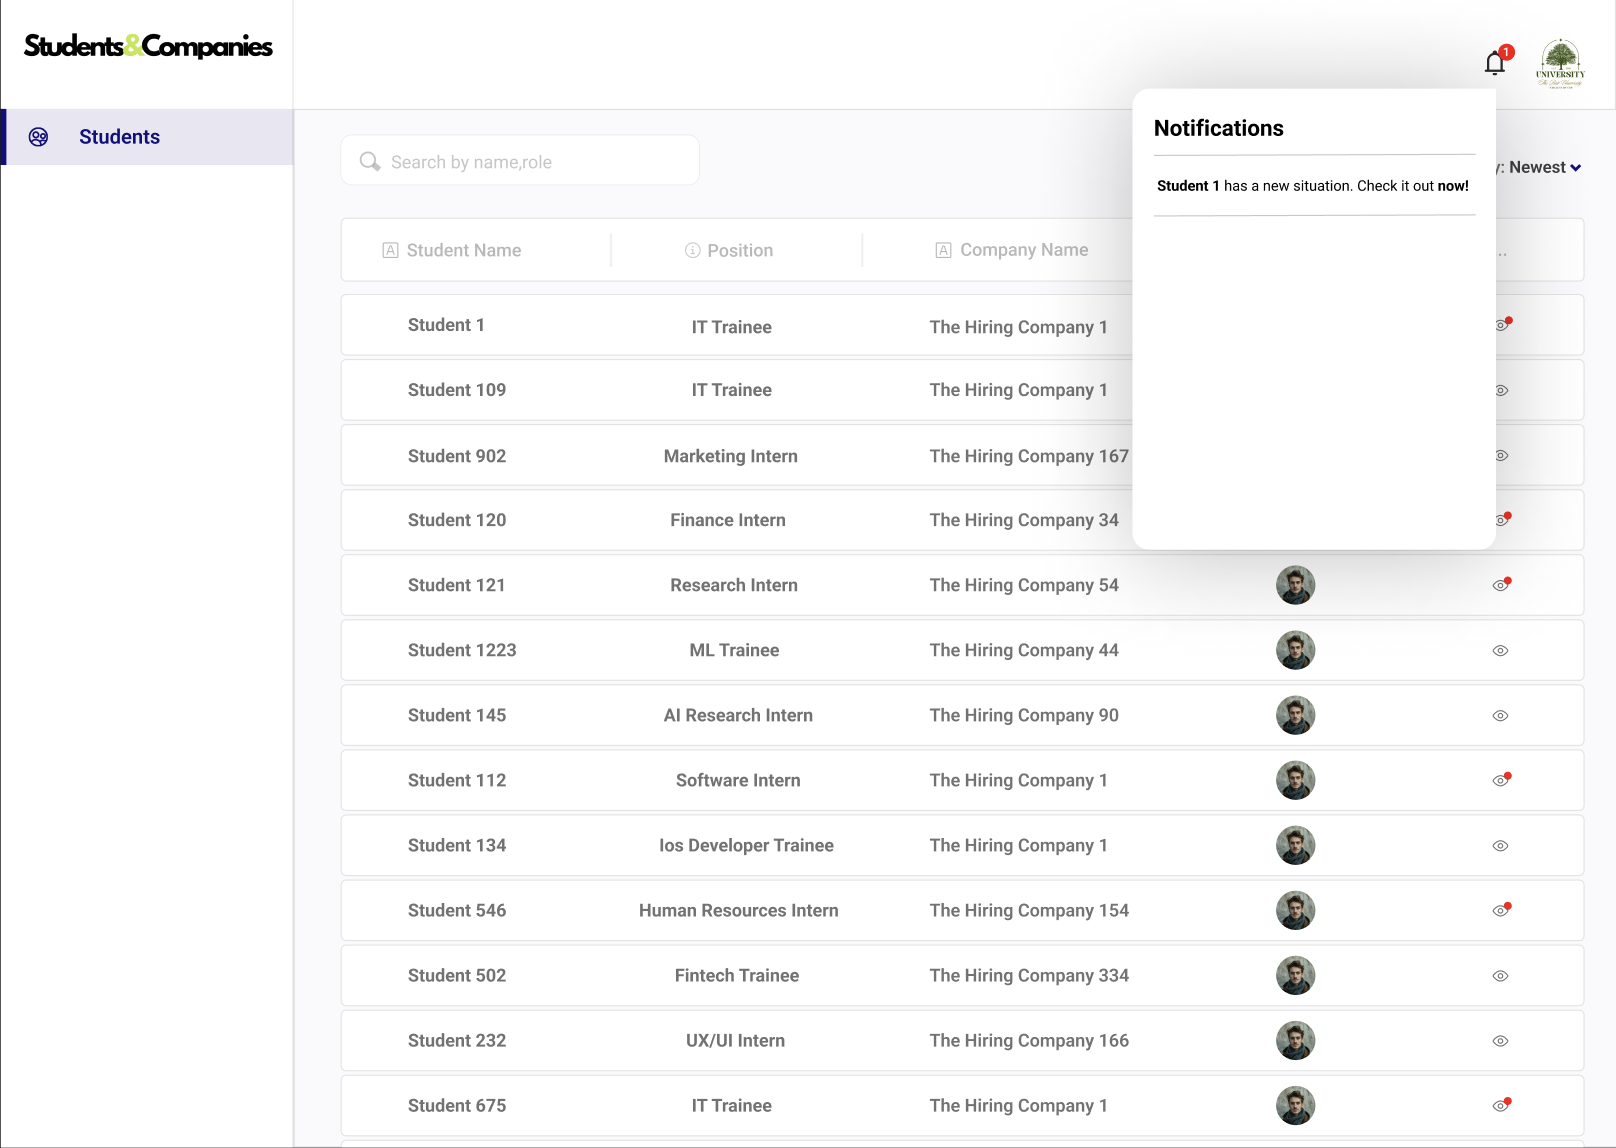
\includegraphics[scale = 0.40]{figures/UserInterfaces/University/University Notifications.png}
    \caption{University Notifications}
     \centering
\end{figure}
\subsubsection{Hardware Interfaces}
    The user, whether a student, university, or company, must use a suitable device to access the system, like a personal computer.
\subsubsection{Software Interfaces}
The system should integrate a NotificationService to keep users updated about any interesting event on
the platform, an EmailService for the registration process, and a proper University Dictionary to ensure the existence of the university.
\subsubsection{Communication Interfaces}
    The system requires a stable internet connection to work properly. This connection is used
    to exchange data between the Users and the central database which contains all the information that is needed for the application to work properly.
\subsection{Functional Requirements}
In this section, all the Use Cases are listed attached to their corresponding Use Case Diagram.
Then, the mapping between Goals, Domain Assumptions and Requirements is provided.
\subsubsection{Use Case Diagrams}
\begin{figure}[H]
    \centering
    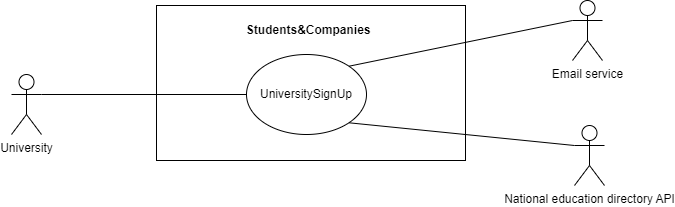
\includegraphics[scale = 0.45]{figures/UseCasesDiagrams/UniversityLogin.drawio.png}
    \caption{UniversitySignUp}
    \centering
\end{figure}
\begin{figure}[H]
    \centering
    \includegraphics[scale = 0.45]{figures/UseCasesDiagrams/CompanySignUp.drawio.png}
    \caption{CompanySignUp}
    \centering
\end{figure}
\begin{figure}[H]
    \centering
    \includegraphics[scale = 0.45]{figures/UseCasesDiagrams/StudentSignUp.drawio.png}
    \caption{StudentSignUp}
    \centering
\end{figure}
\begin{figure}[H]
    \centering
    \includegraphics[scale = 0.45]{figures/UseCasesDiagrams/StudentUC.drawio.png}
    \caption{Student}
    \centering
\end{figure}
\begin{figure}[H]
    \centering
    \includegraphics[scale = 0.4]{figures/UseCasesDiagrams/CompanyUC.drawio.png}
    \caption{Company}
    \centering
\end{figure}
\begin{figure}[H]
    \centering
    \includegraphics[scale = 0.45]{figures/UseCasesDiagrams/use_case_1-University.drawio.png}
    \caption{University}
    \centering
\end{figure}
\begin{figure}[H]
    \centering
    \includegraphics[scale = 0.45]{figures/UseCasesDiagrams/InternshipUC.drawio.png}
    \caption{Internship}
    \centering
\end{figure}
\newpage
\subsubsection{Use cases}
\begin{xltabular}{\textwidth}{| l | X |}
\toprule
\multicolumn{2}{|c|}{StudentsSignUp}\\
\toprule
Participating Actors & Student, Company, EmailService, Students\&Companies, UniversityLoginService, NotificationProvider \\ [1ex]
\hline
Entry Condition & True\\ [1ex]
\hline
Flow of Events & \begin{itemize}
		      \item 1. The Student opens the “Sign up” page
		      \item 2. Students\&Companies shows the page to sign up
		      \item 3. The Student fills the required information and clicks “Sign Up” button
		      \item 4. Students\&Companies checks the information provided by the Student
                \item 5. Students\&Companies shows the university login page through the UniversityLoginService
                \item 6. The Student fills the required information and clicks “Login” button
		      \item 7. UniversityLoginService checks the information provided by the Student
                \item 8. UniversityLoginService confirms the student identity to Students\&Companies
		      \item 9. Students\&Companies registers the Student
                \item 10. Students\&Companies sends confirmation of signup and inform the Student to verify the account
                \item 11. Students\&Companies sends a notification to verify the account through the EmailService
                \item 12. The Student verifies the account
                \item 13. Students\&Companies activates the Student’s account
                \item 14. Students\&Companies might recommend the student to some internships based on the (new) CV.
                \item 15. Students\&Companies sends to the home page. 
                \end{itemize} \\ [1ex]
\hline
Exit Condition & The Student successfully signed up and activated his account\\ [1ex]
\hline
Exceptions & \begin{itemize}
    \item The Student was already registered
    \item  The Student inserts the wrong login credentials
\end{itemize}\\ [1ex]
\hline
\end{xltabular}
\begin{figure}[H]
    \hspace*{-2cm} % Adjust the value (-2cm) to shift left
    \includegraphics[scale = 0.45]{figures/UseCasesSD/StudentSignUpSD.drawio (3).png}\\
\end{figure}

\newpage
\begin{xltabular}{\textwidth}{| l | X |}
\toprule
\multicolumn{2}{|c|}{CompanySignUp}\\
\toprule
Participating Actors & Company, EmailService, Students\&Companies\\ [1ex]
\hline
Entry Condition & True\\ [1ex]
\hline
Flow of Events & \begin{itemize}
		      \item 1. The Company opens the “Sign up” page
		      \item 2. Students\&Companies shows the page to sign up
		      \item 3. The Company fills the required informations and clicks “Require a Company Account” button
		      \item 4. Students\&Companies shows the form to require an Company account
		      \item 5. Students\&Companies registers the Company
                \item 6. Students\&Companies sends confirmation of signup and inform the Company to verify the account
                \item 7. Students\&Companies sends a notification to verify the account through the EmailService
                \item 8. The Company verifies the account
                \item 9. Students\&Companies activates the Company’s account
                \item 10. Students\&Companies sends to the home page 
                \end{itemize} \\ [1ex]
\hline
Exit Condition & The Company successfully signed up and obtained an Company account\\ [1ex]
\hline
Exceptions & The Company was already registered\\ [1ex]
\hline
\end{xltabular}
\begin{figure}[H]
    \centering
    \includegraphics[scale = 0.45]{figures/UseCasesSD/CompanySignUp.drawio.png}\\
\end{figure}

\newpage
\begin{xltabular}{\textwidth}{| l | X |}
\toprule
\multicolumn{2}{|c|}{UniversitySignUp}\\
\toprule
Participating Actors & University, EmailService, National education dictionary
API (NED-API), Students\&Companies\\ [1ex]
\hline
Entry Condition & True\\ [1ex]
\hline
Flow of Events & \begin{itemize}
		      \item 1. The University opens the “Sign up” page
		      \item 2. Students\&Companies shows the page to sign up
		      \item 3. The Company fills the required information and clicks “Require a University Account” button
		      \item 4. Students\&Companies shows the form to require an University account
                \item 5. Students\&Companies check the University existence through he NED-API
		      \item 6. Students\&Companies registers the University
                \item 7. Students\&Companies sends confirmation of sign up and inform the University to verify the account
                \item 8. Students\&Companies sends a notification to verify the account through the EmailService
                \item 9. The University verifies the account
                \item 10. Students\&Companies activates the University’s account
                \item 11. Students\&Companies sends to the home page 
                \end{itemize} \\ [1ex]
\hline
Exit Condition & The University successfully signed up and obtained a University account\\ [1ex]
\hline
Exceptions & \begin{itemize}
                \item The University was already registered
                \item The University does not exist
                \end{itemize} \\ [1ex]
\hline
\end{xltabular}
\begin{figure}[H]
    \centering
    \includegraphics[scale = 0.45]{figures/UseCasesSD/UniversitySignUp.drawio.png}
\end{figure}


\newpage
\begin{xltabular}{\textwidth}{| l | X |}
\toprule
\multicolumn{2}{|c|}{UserLogsIn}\\
\toprule
Participating Actors & User, Students\&Companies\\ [1ex]
\hline
Entry Condition & User has an account\\ [1ex]
\hline
Flow of Events & \begin{itemize}
		      \item 1. The User opens Students\&Companies
		      \item 2. The User clicks the “Log in” button
		      \item 3. Students\&Companies shows the form to log in
		      \item 4. The User fills the required informations and clicks “Log in ” button
		      \item 5. Students\&Companies verifies the credentials of the User
                \item 6. Students\&Companies logs in the User 
                \end{itemize} \\ [1ex]
\hline
Exit Condition & The User successfully logged in\\ [1ex]
\hline
Exceptions & The User filled wrong credentials\\ [1ex]
\hline
\end{xltabular}
\begin{figure}[H]
    \centering
    \includegraphics[scale = 0.45]{figures/UseCasesSD/UserLogsInSD.drawio.png}
\end{figure}


\newpage
\begin{xltabular}{\textwidth}{| l | X |}
\toprule
\multicolumn{2}{|c|}{StudentUpdatesCV}\\
\toprule
Participating Actors & Student, Students\&Companies, Company , NotificationProvider\\ [1ex]
\hline
Entry Condition & The Student is logged in\\ [1ex]
\hline
Flow of Events & \begin{itemize}
		      \item 1. The Student navigates to the profile section
		      \item 2. Students\&Companies displays information about the Student
                \item 3. The Student clicks on the "ModifyCV" button
                \item 4. Students\&Companies displays the "Upload Page"
		      \item 3. The Student uploads a CV file in the provided field.
		      \item 4. Students\&Companies validates the file format and saves the CV file.
                \item 5. Students\&Companies might recommend the student to some internships based on the (new) CV.
                \end{itemize} \\ [1ex]
\hline
Exit Condition & The Student's CV is successfully updated\\ [1ex]
\hline
Exceptions & File upload fails due to incorrect format or size\\ [1ex]
\hline
\end{xltabular}
\begin{figure}[H]
    \centering
    \includegraphics[scale = 0.45]{figures/UseCasesSD/StudentUpdatesCV.drawio.png}
\end{figure}



\newpage
\begin{xltabular}{\textwidth}{| l | X |}
\toprule
\multicolumn{2}{|c|}{StudentChangesUniversity}\\
\toprule
Participating Actors & Student, Students\&Companies, UniversityLoginService, EmailService\\ [1ex]
\hline
Entry Condition & The Student is logged in and has an active account\\ [1ex]
\hline
Flow of Events & \begin{itemize}
		      \item 1. The Student navigates to the “Profile” section
		      \item 2. Students\&Companies displays information about the Student
		      \item 3. The Student selects the mail field and overwrites the email with the one from the new from the other University
                \item 4. Students\&Companies shows the university login page through the UniversityLoginService
                \item 5. The Student fills the required information and clicks “Login” button
		      \item 6. UniversityLoginService checks the information provided by the Student
                \item 7. UniversityLoginService confirms the student identity to Students\&Companies
                \item 8. Students\&Companies saves the new Student’s email
                \item 9. Students\&Companies sends confirmation of signup and inform the Student to verify the email
                \item 10. Students\&Companies sends a notification to verify the email through the EmailService
                \item 11. The Student verifies the email
		      \item 12. Students\&Companies validates the university information
                \end{itemize} \\ [1ex]
\hline
Exit Condition & The Student's university information is successfully updated\\ [1ex]
\hline
Exceptions & The Student inserts the wrong login credentials\\ [1ex]
\hline
\end{xltabular}
\begin{figure}[H]
    \centering
    \includegraphics[scale = 0.45]{figures/UseCasesSD/StudentChangesUniversitySD.drawio (1).png}
\end{figure}


\newpage
\begin{xltabular}{\textwidth}{| l | X |}
\toprule
\multicolumn{2}{|c|}{CompanyPostsInternship}\\
\toprule
Participating Actors & Company, NotificationService, Student, Students\&Companies\\ [1ex]
\hline
Entry Condition & The Company is logged in\\ [1ex]
\hline
Flow of Events & \begin{itemize}
		      \item 1. The Company clicks on to the “Post Internship” button
		      \item 2. Students\&Companies displays the internship creation form
		      \item 3. The Company fills out the form with internship details and submits it
		      \item 4. Students\&Companies validates the information and publishes the internship
                \item 5. the NotificationService may notify certain students of this new internship through recommendation
                \end{itemize} \\ [1ex]
\hline
Exit Condition & The internship is successfully posted and visible to Students\\ [1ex]
\hline
Exceptions & Incomplete internship details provided\\ [1ex]
\hline
\end{xltabular}
\begin{figure}[H]
    \centering
    \includegraphics[scale = 0.45]{figures/UseCasesSD/CompanyPostsInternshipSD.drawio.png}
\end{figure}


\newpage
\begin{xltabular}{\textwidth}{| l | X |}
\toprule
\multicolumn{2}{|c|}{UserReccomendationFeedback }\\
\toprule
Participating Actors & User (Student or Company), Students\&Companies\\ [1ex]
\hline
Entry Condition & The User is logged into the platform\\ [1ex]
\hline
Flow of Events & \begin{itemize}
		      \item 1. The Student navigates to the homepage. The Company selects one of its posted Internships.
                \item 2. The User selects the "thumb-up" or the "thumb-down" button.
		      \item 3. Students\&Companies registers the preference and updates the recommendation system.
                \end{itemize} \\ [1ex]
\hline
Exit Condition & The User feedback is taken into account for future recommendations.\\ [1ex]
\hline
\end{xltabular}
\begin{figure}[H]
    \centering
    \includegraphics[scale = 0.45]{figures/UseCasesSD/UserReccomendationFeedbackSD.drawio.png}
\end{figure}

\newpage
\begin{xltabular}{\textwidth}{| l | X |}
\toprule
\multicolumn{2}{|c|}{StudentAppliesToInternship}\\
\toprule
Participating Actors & Student, Students\&Companies\\ [1ex]
\hline
Entry Condition & The Student is logged in\\ [1ex]
\hline
Flow of Events & \begin{itemize}
		      \item 1. The Student types in the search bar the internship or the company that he would like to intern at.
		      \item 2. Students\&Companies retrieves and displays matching available internships.
                \item 3. The Student clicks on an Internship.
                \item 4. Students\&Companies sh ows the Internship's profile details.
                \item 5. The Student clicks on the "Apply" button.
                \item 6. Students\&Companies performs the student application and adds the student to the list of applicants of the related company.
                \end{itemize} \\ [1ex]
\hline
Exit Condition & The Student views a list of internships matching their criteria\\ [1ex]
\hline
Exceptions & No internships match the search criteria\\ [1ex]
\hline
\end{xltabular}
\begin{figure}[H]
    \centering
    \includegraphics[scale = 0.45]{figures/UseCasesSD/StudentAppliesToIntershipSD.drawio (1).png}
\end{figure}

\newpage
\begin{xltabular}{\textwidth}{| l | X |}
\toprule
\multicolumn{2}{|c|}{UserSelectsInternship}\\
\toprule
Participating Actors & User (Student, Company, or University), Students\&Companies\\ [1ex]
\hline
Entry Condition & The User is logged in\\ [1ex]
\hline
Flow of Events & \begin{itemize}
		      \item 1. The User access the homepage of the platform
		      \item 2. Students\&Companies displays: to the companies their posted internships to the students the ones recommended by the system and to universities the ongoing ones in which their students are taking part. 
		      \item 3. The User clicks on one of the shown internships from the list.
		      \item 4. Students\&Companies displays all the information about the selected internship.
                \end{itemize} \\ [1ex]
\hline
Exit Condition & The user visualizes the current information about the internship\\ [1ex]
\hline
Exceptions & None\\ [1ex]
\hline
\end{xltabular}
\begin{figure}[H]
    \centering
    \includegraphics[scale = 0.45]{figures/UseCasesSD/UserSelectsIntenrshipSD.drawio.png}
\end{figure}



\newpage
\begin{xltabular}{\textwidth}{| l | X |}
\toprule
\multicolumn{2}{|c|}{StudentAcceptsCompany}\\
\toprule
Participating Actors & Student, Students\&Companies\\ [1ex]
\hline
Entry Condition & The Student is Logged in\\ [1ex]
\hline
Flow of Events & \begin{itemize}
                \item 1. The Student selects one of the recommended internships.
                \item 2. Students\&Companies displays all the information regarding the Internship.
                \item 5. The Student clicks on the "Accept" button. 
                \item 6. Students\&Companies registers the Student acceptance accordingly.
                \end{itemize} \\ [1ex]
\hline
Exit Condition & The Company successfully accepted the Student for one of its posted internships.\\ [1ex]
\hline
Exceptions & None \\ [1ex]
\hline
\end{xltabular}
\begin{figure}[H]
    \centering
    \includegraphics[scale = 0.45]{figures/UseCasesSD/StudentAcceptsReccomendationSD.drawio.png}
\end{figure}


\newpage
\begin{xltabular}{\textwidth}{| l | X |}
\toprule
\multicolumn{2}{|c|}{CompanyAcceptsStudent}\\
\toprule
Participating Actors & Company, Students\&Companies\\ [1ex]
\hline
Entry Condition & The Company is Logged in\\ [1ex]
\hline
Flow of Events & \begin{itemize}
                \item 1. The Company selects one of its posted internship. 
		      \item 2. Students\&Companies displays the list of all the recommended and applicant students for that internship.
		      \item 3. The Company selects one of the Student from the list. 
                \item 4. Students\&Companies displays all the information regarding the Student.
                \item 5. The Company clicks on the "Accept" button. 
                \item 6. Students\&Companies registers the Company acceptance accordingly.
                \end{itemize} \\ [1ex]
\hline
Exit Condition & The Company successfully accepted the Student for one of its posted internships.\\ [1ex]
\hline
Exceptions & None \\ [1ex]
\hline
\end{xltabular}
\begin{figure}[H]
    \centering
    \includegraphics[scale = 0.45]{figures/UseCasesSD/CompanyAcceptsStudentSD.drawio (1).png}
\end{figure}


\newpage
\begin{xltabular}{\textwidth}{| l | X |}
\toprule
\multicolumn{2}{|c|}{CompanySchedulesInterview}\\
\toprule
Participating Actors & Company, Students\&Companies, NotificationProvider, Student\\ [1ex]
\hline
Entry Condition & The company is logged in and has at least one internship whose application deadline is expired.\\ [1ex]
\hline
Flow of Events & \begin{itemize}
		      \item 1. The Company selects one of its posted internship whose application deadline is expired. 
		      \item 2. Students\&Companies displays a time span form.
		      \item 3. The Company fills the form in giving the dates and timings that it will use for interview.
		      \item 4. Students\&Companies splits the given time span in slots of equal size according to the number of candidates.
                \item 5. the NotificationService notifies all candidates of the interview time-slots availability.
                \item 6. Students\&Companies shows to the company the list  of candidates and for each the associated time-slot preference if they have already chosen one.
                \end{itemize} \\ [1ex]
\hline
Exit Condition & The company has successfully scheduled the interview periods.\\ [1ex]
\hline
Exceptions & None\\ [1ex]
\hline
\end{xltabular}
\begin{figure}[H]
    \centering
    \includegraphics[scale = 0.45]{figures/UseCasesSD/CompanySchedulesInterviewSD.drawio.png}
\end{figure}

\newpage
\begin{xltabular}{\textwidth}{| l | X |}
\toprule
\multicolumn{2}{|c|}{StudentSchedulesInterview}\\
\toprule
Participating Actors & Student, Students\&Companies\\ [1ex]
\hline
Entry Condition & The Student is logged in, he is a candidate for an internship and has received a notification about the availability of time-slots for that internship.\\ [1ex]
\hline
Flow of Events & \begin{itemize}
		      \item 1. The Student selects the internship he has been notified of.
		      \item 2. Students\&Companies shows a form containing the available time-slots to book for the interview with that internship.
		      \item 3. The Student selects a time slot and submits the form.
		      \item 4. Students\&Companies registers the choice.
                \end{itemize} \\ [1ex]
\hline
Exit Condition & The Student has successfully booked a time slot for the internship interview.\\ [1ex]
\hline
Exceptions & None\\ [1ex]
\hline
\end{xltabular}
\begin{figure}[H]
    \centering
    \includegraphics[scale = 0.45]{figures/UseCasesSD/StudentSchedulesInterviewSD2.drawio.png}
\end{figure}

\newpage
\begin{xltabular}{\textwidth}{| l | X |}
\toprule
\multicolumn{2}{|c|}{CompanySelectsCandidate}\\
\toprule
Participating Actors & Company, Students\&Companies, NottificationProvider, Student\\ [1ex]
\hline
Entry Condition & The Company is Logged in\\ [1ex]
\hline
Flow of Events & \begin{itemize}
                \item 1. The Company selects one of its posted internship with expired deadline. 
		      \item 2. Students\&Companies displays the list of all the candidate students for that internship.
		      \item 3. The Company selects one of the Student from the list. 
                \item 4. Students\&Companies displays all the information regarding the Student.
                \item 5. The Company clicks on the "Select" button. 
                \item 6. Students\&Companies registers the Company selection for that internship and waits for the student confirmation.
                \item 7. The NotificationService notifies the selected Student of his selection.
                \item 8. Students\&Companies changes the button changes the .
                \end{itemize} \\ [1ex]
\hline
Exit Condition & The Company successfully selected the Student for one of its posted internships.\\ [1ex]
\hline
Exceptions & None \\ [1ex]
\hline
\end{xltabular}
\begin{figure}[H]
    \centering
    \includegraphics[scale = 0.45]{figures/UseCasesSD/CompanySelectsCandidateSD.drawio (1).png}
\end{figure}
\newpage
\begin{xltabular}{\textwidth}{| l | X |}
\toprule
\multicolumn{2}{|c|}{StudentconfirmsSelection}\\
\toprule
Participating Actors & Company, Students\&Companies, NottificationProvider, Student\\ [1ex]
\hline
Entry Condition & The Student is Logged in\\ [1ex]
\hline
Flow of Events & \begin{itemize}
                \item 1. The Student clicks on the Internship that selected him. 
                \item 2. Students\&Companies displays the selection confirmation form.
                \item 3. The Student clicks on the "Confirm" or the "Reject" button accordingly to his will. 
                \item 4. Students\&Companies registers the Student choice for that internship.
                \item 5. The NotificationService notifies the providing Company about the selcetion choice.
                \end{itemize} \\ [1ex]
\hline
Exit Condition & The Student successfully chooses if to confirm or reject his participation to the Intenrship. The providing company gets informed accordingly.\\ [1ex]
\hline
Exceptions & None \\ [1ex]
\hline
\end{xltabular}
\begin{figure}[H]
    \centering
    \includegraphics[scale = 0.45]{figures/UseCasesSD/StudentconfirmsSelectionSD.drawio.png}
\end{figure}


\newpage
\begin{xltabular}{\textwidth}{| l | X |}
\toprule
\multicolumn{2}{|c|}{UserViewsComments}\\
\toprule
Participating Actors & User (Student, Company, or University), Students\&Companies\\ [1ex]
\hline
Entry Condition & The User is logged into the platform\\ [1ex]
\hline
Flow of Events & \begin{itemize}
		      \item 1. The User navigates to the internship page he has been selected for.
                \item 1. The User navigets to the "View Comments" section
		      \item 2. Students\&Companies retrieves the comments associated with the relevant internship
		      \item 3. Students\&Companies displays the comments to the User
                \end{itemize} \\ [1ex]
\hline
Exit Condition & The User views all comments for the selected internship\\ [1ex]
\hline
Exceptions & No comments are available for the internship\\ [1ex]
\hline
\end{xltabular}
\begin{figure}[H]
    \centering
    \includegraphics[scale = 0.7]{figures/UseCasesSD/UserViewsCommentsSD.png}
\end{figure}




\newpage
\begin{xltabular}{\textwidth}{| l | X |}
\toprule
\multicolumn{2}{|c|}{UserWritesComment}\\
\toprule
Participating Actors & User (Student or Company), NotificationService, Students\&Companies\\ [1ex]
\hline
Entry Condition & The User is logged into the platform\\ [1ex]
\hline
Flow of Events & \begin{itemize}
		      \item 1. The User navigates to the “Write Comment” section
		      \item 2. Students\&Companies displays the comment input form
		      \item 3. The User writes the comment and submits it
		      \item 4. Students\&Companies validates the input and saves the comment
		      \item 5. Students\&Companies notifies the relevant User (Student or Company) of the new comment
                \end{itemize} \\ [1ex]
\hline
Exit Condition & The comment is successfully saved and notified to the other party\\ [1ex]
\hline
Exceptions & The comment is invalid (e.g., empty or contains restricted content)\\ [1ex]
\hline
\end{xltabular}
\newpage
\begin{figure}[H]
    \centering
    \includegraphics[scale = 0.9]{figures/UseCasesSD/UserWritesObservationSD.png}
\end{figure}

\begin{figure}[H]
    \centering
    \includegraphics[scale = 0.75]{figures/UseCasesSD/UserWritesComplaintSD.png}
\end{figure}

\newpage
\begin{xltabular}{\textwidth}{| l | X |}
\toprule
\multicolumn{2}{|c|}{UniversityInterruptsInternship}\\
\toprule
Participating Actors & University, NotificationService,  Students\&Companies\\ [1ex]
\hline
Entry Condition & The University has logged in and is in home page \\ [1ex]
\hline
Flow of Events & \begin{itemize}
		      \item 1. The University selects a flagged internship 
                \item 2. the University clicks the button to interrupt the internship
		      \item 3. Students\&Companies interrupts the internship and notifies the Student and the Company
                \end{itemize} \\ [1ex]
\hline
Exit Condition & The internship is interrupted and both parties are notified\\ [1ex]
\hline
Exceptions & The University cannot interrupt an internship already completed\\ [1ex]
\hline
\end{xltabular}
\begin{figure}[H]
    \centering
    \includegraphics[scale = 0.75]{figures/UseCasesSD/UniversityInterruptsInternshipSD.png}
\end{figure}


\newpage
\begin{xltabular}{\textwidth}{| l | X |}
\toprule
\multicolumn{2}{|c|}{UserSubmitsFeedback}\\
\toprule
Participating Actors & User (Company or Student), Students\&Companies\\ [1ex]
\hline
Entry Condition & The user is logged in and one of the internship he participated in has just finished.\\ [1ex]
\hline
Flow of Events & \begin{itemize}
		      \item 1. The User opens the internship page
		      \item 2. Students\&Companies displays a feedback form containing five possibilities.
		      \item 3. The User chooses one of the five possibilities and submits the feedback.
		      \item 4. Students\&Companies closes and archives the internship after both the company adn the student have submitted the feedback.
                \end{itemize} \\ [1ex]
\hline
Exit Condition & The internship was archived successfully\\ [1ex]
\hline
Exceptions & None\\ [1ex]
\hline
\end{xltabular}
\begin{figure}[H]
    \centering
    \includegraphics[scale = 0.45]{figures/UseCasesSD/UserSubmitsFeedbackSD.drawio.png}
\end{figure}
\newpage

\subsubsection{Mapping}
\begin{center}
    \begin{tabular}{|C{3cm}|p{10cm}|}
    \hline
    \multicolumn{2}{|c|}{\parbox{13cm}{G1: Allows registered companies to post and advertise the available internships that they offer.}} \\
    \hline
    \centering R1 & The system must allow a student who wants to register to sign up. \\ 
    \hline
    \centering R2 & The system must allow a company who wants to register to sign up. \\ 
    \hline
    \centering R4 & The system must allow registered users to sign in using their credentials. \\ 
    \hline
    \centering R7 & The system must allow registered students to enter information from their CV to complete their profiles. \\ 
    \hline
    \centering R8 & The system must allow registered companies to post internship advertisements. \\ 
    \hline
    \centering R9 & The system must allow companies to review students' CVs and select candidates who meet their internship requirements. \\ 
    \hline
    \centering R10 & The system must allow students to review internship advertisements and select them if they wish to apply. \\ 
    \hline
    \centering R12 & The system must notify students when there are updates regarding the internships they applied for or accepted. \\ 
    \hline
    \centering R16 & The system must recommend a student and a company profile to each other and allow them to review whether the company has an active internship position and if the profiles could attract each other's interest. \\ 
    \hline
    \centering R21 & The system must notify students when there are updates regarding the results of the internships they have applied for. \\ 
    \hline
    \centering R24 & The system must allow companies to view and manage applications for the internships they have posted. \\ 
    \hline
    \centering R25 & The system must allow students to view all details about the internships they have applied for, such as completion status, and deadlines. \\ 
    \hline
    \centering D4 & A university needs to be registered for its students to link their accounts and start applying for internships. \\ 
    \hline
    \end{tabular}
\end{center}


    
\begin{center}
    \begin{tabular}{|C{3cm}|p{10cm}|}
    \hline
    \multicolumn{2}{|c|}{\parbox{13cm}{G2: Allows registered students to proactively and autonomously search and apply internships.}} \\
    \hline
    \centering R1 & The system must allow a student who wants to register to sign up. \\ 
    \hline
    \centering R4 & The system must allow registered users to sign in using their credentials. \\ 
    \hline
    \centering R7 & The system must allow registered students to enter information from their CV to complete their profiles. \\ 
    \hline
    \centering R11 & The system must allow students to manually search for internship opportunities and apply for them. \\ 
    \hline
    \centering D4 & A university needs to be registered for its students to link their accounts and start applying for internships. \\ 
    \hline
    \end{tabular}
\end{center}


\begin{center}
    \begin{tabular}{|C{3cm}|p{10cm}|}
    \hline
    \multicolumn{2}{|c|}{\parbox{13cm}{G3: Helps registered students and registered companies by suggesting them appealing templates for their CVs and internship projects drafts.}} \\
    \hline
    \centering R1 & The system must allow a student who wants to register to sign up. \\ 
    \hline
    \centering R2 & The system must allow a company who wants to register to sign up. \\ 
    \hline
    \centering R4 & The system must allow registered users to sign in using their credentials. \\ 
    \hline
    \centering R6 & The system must be able to send notifications to all users. \\ 
    \hline
    \centering R7 & The system must allow registered students to enter information from their CV to complete their profiles. \\ 
    \hline
    \centering R8 & The system must allow registered companies to post internship advertisements. \\ 
    \hline
    \centering R18 & The system must allow companies to evaluate students during the internship process and provide feedback on their CVs. \\ 
    \hline
    \centering R20 & The system must provide suggestions to users for improving their profiles based on feedback. \\ 
    \hline
    \centering D4 & A university needs to be registered for its students to link their accounts and start applying for internships. \\ 
    \hline
    \end{tabular}
\end{center}


\begin{center}
    \begin{tabular}{|C{3cm}|p{10cm}|}
    \hline
    \multicolumn{2}{|c|}{\parbox{13cm}{G4: Allows a registered student to be recommended a list of advertised internships that might be of interest to him/her with respect to: his/her uploaded CV, the internships projects, and users' feedbacks.}} \\
    \hline
    \centering R1 & The system must allow a student who wants to register to sign up. \\ 
    \hline
    \centering R2 & The system must allow a company who wants to register to sign up. \\ 
    \hline
    \centering R3 & The system must allow a university who wants to register to sign up. \\ 
    \hline
    \centering R4 & The system must allow registered users to sign in using their credentials. \\ 
    \hline
    \centering R6 & The system must be able to send notifications to all users. \\ 
    \hline
    \centering R7 & The system must allow registered students to enter information from their CV to complete their profiles. \\ 
    \hline
    \centering R8 & The system must allow registered companies to post internship advertisements. \\ 
    \hline
    \centering D4 & A university needs to be registered for its students to link their accounts and start applying for internships. \\ 
    \hline
    \end{tabular}
\end{center}

\begin{center}
    \begin{tabular}{|C{3cm}|p{10cm}|}
    \hline
    \multicolumn{2}{|c|}{\parbox{13cm}{G5: Allows a registered company to be recommended a list of registered students who might be of interest for one of its advertised internships with respect to: their uploaded CVs, the internship project and users' feedbacks.}} \\
    \hline
    \centering R1 & The system must allow a student who wants to register to sign up. \\ 
    \hline
    \centering R2 & The system must allow a company who wants to register to sign up. \\ 
    \hline
    \centering R3 & The system must allow a university who wants to register to sign up. \\ 
    \hline
    \centering R4 & The system must allow registered users to sign in using their credentials. \\ 
    \hline
    \centering R7 & The system must allow registered students to enter information from their CV to complete their profiles. \\ 
    \hline
    \centering R8 & The system must allow registered companies to post internship advertisements. \\ 
    \hline
    \centering D4 & A university needs to be registered for its students to link their accounts and start applying for internships. \\ 
    \hline
    \end{tabular}
\end{center}

\begin{center}
    \begin{tabular}{|C{3cm}|p{10cm}|}
    \hline
    \multicolumn{2}{|c|}{\parbox{13cm}{G6: Allows a registered company to view the list of all the students who applied to one of its advertised internships grouped by the internship they applied to.}} \\
    \hline
    \centering D4 & A university needs to be registered for its students to link their accounts and start applying for internships. \\ 
    \hline
    \end{tabular}
\end{center}

\begin{center}
    \begin{tabular}{|C{3cm}|p{10cm}|}
    \hline
    \multicolumn{2}{|c|}{\parbox{13cm}{G7: Allows a registered student to access the list of internships that he/she has applied for and the ones that he/she has accepted, along with deadlines and other important details.}} \\
    \hline
    \centering R4 & The system must allow registered users to sign in using their credentials. \\ 
    \hline
    \centering R7 & The system must allow registered students to enter information from their CV to complete their profiles. \\ 
    \hline
    \centering R10 & The system must allow students to review internship advertisements and select them if they wish to apply. \\ 
    \hline
    \centering R25 & The system must allow students to view all details about the internships they have applied for, such as completion status, and deadlines. \\ 
    \hline
    \centering D4 & A university needs to be registered for its students to link their accounts and start applying for internships. \\ 
    \hline
    \end{tabular}
\end{center}

\begin{center}
    \begin{tabular}{|C{3cm}|p{10cm}|}
    \hline
    \multicolumn{2}{|c|}{\parbox{13cm}{G8: Allows a registered company to access the list of students that applied to its internships and the status of each student's application (rejected, selected, etc.).}} \\
    \hline
    \centering R4 & The system must allow registered users to sign in using their credentials. \\ 
    \hline
    \centering R8 & The system must allow registered companies to post internship advertisements. \\ 
    \hline
    \centering R9 & The system must allow companies to review students' CVs and select candidates who meet their internship requirements. \\ 
    \hline
    \centering R16 & The system must recommend a student and a company profile to each other and allow them to review whether the company has an active internship position and if the profiles could attract each other's interest. \\ 
    \hline
    \centering D4 & A university needs to be registered for its students to link their accounts and start applying for internships. \\ 
    \hline
    \end{tabular}
\end{center}

\begin{center}
    \begin{tabular}{|C{3cm}|p{10cm}|}
    \hline
    \multicolumn{2}{|c|}{\parbox{13cm}{G9: Allows a registered student to view a list of available internships sorted by company, internship description, deadline, and application status.}} \\
    \hline
    \centering R4 & The system must allow registered users to sign in using their credentials. \\ 
    \hline
    \centering R7 & The system must allow registered students to enter information from their CV to complete their profiles. \\ 
    \hline
    \centering R10 & The system must allow students to review internship advertisements and select them if they wish to apply. \\ 
    \hline
    \centering R12 & The system must notify students when there are updates regarding the internships they applied for or accepted. \\ 
    \hline
    \centering D4 & A university needs to be registered for its students to link their accounts and start applying for internships. \\ 
    \hline
    \end{tabular}
\end{center}

\begin{center}
    \begin{tabular}{|C{3cm}|p{10cm}|}
    \hline
    \multicolumn{2}{|c|}{\parbox{13cm}{G10: Allows a registered company to track and update the application status of students applying to its internships.}} \\
    \hline
    \centering R4 & The system must allow registered users to sign in using their credentials. \\ 
    \hline
    \centering R8 & The system must allow registered companies to post internship advertisements. \\ 
    \hline
    \centering R9 & The system must allow companies to review students' CVs and select candidates who meet their internship requirements. \\ 
    \hline
    \centering R15 & The system must allow companies to provide feedback to students regarding their application status. \\ 
    \hline
    \centering R27 & The system must allow universities to follow internship processes, handle complaints raised by students, and interrupt an internship if necessary. \\ 
    \hline
    \centering D4 & A university needs to be registered for its students to link their accounts and start applying for internships. \\ 
    \hline
    \end{tabular}
\end{center}

\begin{center}
    \begin{tabular}{|C{3cm}|p{10cm}|}
    \hline
    \multicolumn{2}{|c|}{\parbox{13cm}{G11: Allows registered students and companies to communicate with each other regarding internship applications and statuses.}} \\
    \hline
    \centering R4 & The system must allow registered users to sign in using their credentials. \\ 
    \hline
    \centering R8 & The system must allow registered companies to post internship advertisements. \\ 
    \hline
    \centering R10 & The system must allow students to review internship advertisements and select them if they wish to apply. \\ 
    \hline
    \centering R12 & The system must notify students when there are updates regarding the internships they applied for or accepted. \\ 
    \hline
    \centering R14 & The system must allow students to contact companies regarding the internships they applied for. \\ 
    \hline
    \centering D4 & A university needs to be registered for its students to link their accounts and start applying for internships. \\ 
    \hline
    \end{tabular}
\end{center}



	
	

   


\subsection{Performance Requirements}
Due to the non-critical nature of the system, strict performance requirements are not needed. Nonetheless, for the best user experience these are the set requirements:
\begin{itemize}
    \item The system should let Companies create an Internship within 2 seconds.
    \item The system should let Students upload their CV within 2 seconds.
    \item The system should let Students accept an Internship recommendation within 2 seconds.
    \item The system should let Companies accept a Student recommendation within 2 seconds.
    \item The system should reload the Users recommendations within 5 seconds after a user feedback submission.
    \item The system should let Companies fix the interview time slots accordingly within 2 seconds.
    \item The system should let Students select their preferred interview time slot within 2 seconds. 
    \item The system should let Companies select their preferred internship candidate within 2 seconds.
    \item The system should let Companies and Students post comments within 2 seconds.
    \item The system should let Universities interrupt internships within 5 seconds. \\
\end{itemize}

\subsection{Design Constraints}
\subsubsection{Standards compliance}
Specifications described in this document must be respected by the system. The source code
of the application must be commented on and documented adequately.
The system should respect the guidelines described by the GDPR.
\subsubsection{Hardware limitations}
The system requires any device and a stable internet connection.
\subsection{Software System Attributes}

\subsubsection{Reliability and Availability}
The system should guarantee an availability equal to 99.5 or more\%. In
other words, the system will be inaccessible for less than two days every year. To achieve this
goal, a high redundancy for the critical components will be ensured.
Furthermore, in order to guarantee better reliability performances, all the scheduled mainte-
nance actions on the system should be done during the night.
\subsubsection{Security}
The connection between the application and the server must be safe. To keep a good level of
security, the system should use the Transport Layer Security protocol. For this purpose, it is
needed an SSL/TSL certificate.
\subsubsection{Maintainability}
The source code must be commented on as well as possible and the correlated documentation
must be kept updated during the whole life cycle of the system.
Modularity and low coupling between components must be a focus during the designing and
developing phases.

\section{Formal Analysis Using Alloy}
\subsection{Objectives of the Analysis}
This section presents the formal modeling activity conducted using Alloy notation. The primary objective of this work is to provide a rigorous description of the system's domain and its properties.
The main objective of the formal modeling activity is to ensure the correctness, consistency, and efficiency of the platform. By formally modeling key aspects of the system using Alloy, we aim to verify that the system behaves as intended under various conditions and check complex relationships and constraints between entities.

The main aspects that can be proven are:
\begin{itemize}
    \item Mutual Recommendation and Acceptance
    \item Concurrency Constraints
    \item Internship State Transitions
    \item Correctness of Feedback Submission
    \item Correctness of Comment Submission
\end{itemize}
\subsection{Description of the Model}
The model captures the following key features:
\begin{itemize}
    \item Users and Roles:
    The model distinguishes between three types of users: Student, University, and Company. These users interact with internships in different ways, with students applying to internships, accepting recommendations, and leaving feedback. While, universities manage student data and can interrupt internships.
    \item Internships:
    Internships are the central object in the system, with states that reflect their progression from Application to Ended. Each internship has a status, an applicationDeadline, a startingDate, an endingDate, comments and feedbacks.
    \item Relationships and Constraints.
    Several constraints govern the interactions between users and internships.
\end{itemize}
\subsection{Relevance}
Modeling the platform in this way is important for two main reasons. Consistency and scalability.

Consistency is ensured by verifying constraints on internship transitions and user interactions. This guarantees that the platform behaves predictably, reducing the risk of system malfunctions and avoids conflicting actions.

On the other hand, facilitating scalability is equally important. The model ensures that the system remains robust even in scenarios with multiple internships and users interactions. In this way, we can avoid performance bottlenecks and ensure that the platform can scale efficiently without introducing errors.
\subsection{Alloy Code}

\subsubsection{Definition of actors, components and auxiliar entities}
\begin{lstlisting}
// Abstract signature representing a generic user in the system
abstract sig User {}

// A student is a type of user with relationships to internships
sig Student extends User {
    reccomended: some Internship, // Internships recommended to the student
    appliesTo: set Internship,   // Internships the student has applied to
    accepts: set Internship      // Internships the student has accepted
} {
    accepts in reccomended        // Students can only accept recommended internships
    appliesTo & accepts = none    // Applied and accepted internships must not overlap
}

// A university is a user that manages students
sig University extends User {
    students: some Student         // Students associated with the university
}

// A company is a user that manages internships
sig Company extends User {}

// Represents the current moment in time
one sig CurrentDate {
    time: one Int                 // Current time as an integer value
}

// Represents a specific point in time (e.g., deadlines, start dates)
sig Date {
    time: one Int                 // Time as an integer value
}

// Enumeration of possible internship statuses
enum InternshipStatus {Application, Selection, Ongoing, Feedback, Ended, Interrupted}

// Represents an internship with various attributes and constraints
sig Internship {
    status: one InternshipStatus,  // Current status of the internship
    managedBy: one Company,        // The company managing the internship
    reccomended: some Student,     // Students recommended for the internship
    accepted: set Student,         // Students whose recommendation was accepted
    candidates: set Student,       // Students mutually accepted for selection
    selected: lone Student,        // Selected student (if any)
    applicationDeadline: one Date, // Application deadline
    startingDate: one Date,        // Internship start date
    endingDate: one Date,          // Internship end date
    comments: set Comment,         // Comments on the internship
    feedbacks: set Feed,           // Feedback associated with the internship
    interruptedBy: lone University // University that interrupted the internship (if any)
} {
    applicationDeadline.time < startingDate.time      // Valid time constraints
    startingDate.time < endingDate.time
    accepted in reccomended                          // Accepted students must be recommended
    candidates in accepted                           // Candidates must be among accepted students
    selected in candidates                           // Selected student must be among candidates
    interruptedBy != none implies (selected in interruptedBy.students and some c : comments | c.complaint = True)
}

// Enumeration for boolean values
enum Boolean {True, False}

// Represents a comment made by a user
sig Comment {
    wroteBy: one User,          // User who wrote the comment
    complaint: one Boolean      // Indicates if the comment is a complaint
} {
    wroteBy & University = none // Universities cannot write comments
    complaint = True implies wroteBy & Company = none // Complaints cannot come from companies
}

// Abstract signature representing generic feedback in the system
abstract sig Feed {
    submittedBy: one User       // User who submitted the feedback
} {
    submittedBy in User - University // Universities cannot submit feedback
}

// Feedback submitted by students and companies after the internship
sig RatingFeedback extends Feed {
    stars: one Int              // Rating value
} {
    stars >= 0 and stars <= 5   // Ratings must be between 0 and 5
}

// Enumeration for thumbs-up or thumbs-down feedback
enum Thumb {Up, Down}

// Feedback about recommendations given by students and companies
abstract sig ReccomendationFeedback extends Feed { preference: one Thumb }

sig ReccomendationCompany extends ReccomendationFeedback {
	relatedTo: one Student
}{
	submittedBy in Company
	relatedTo in Internship.reccomended
}

sig ReccomendationStudent extends ReccomendationFeedback {} 
{submittedBy in Student}

\end{lstlisting}

\subsubsection{Facts}

\begin{lstlisting}
fact commentExistance {
    all c : Comment |
    one i : Internship | c in i.comments
}

fact commentConstring {
    all i : Internship | 
    all c : Comment |
    c in i.comments iff
    c.wroteBy in (i.selected + i.managedBy) and i.selected != none and 
    i.status != Application and i.status != Selection
}

fact feedbackExistance {
    all f : Feed |
    one i : Internship | f in i.feedbacks
}

fact ratingConstraint {
    all i : Internship |
    all f : RatingFeedback |
    f in i.feedbacks iff
    f.submittedBy in (i.selected + i.managedBy) and (i.status = Feedback or i.status = Ended)
}

fact recommendationConstraint {
    all disj f1, f2:  ReccomendationCompany | f1.submittedBy = f2.submittedBy implies f1.relatedTo != f2.relatedTo
}

fact companyRecommendationConstraint {
	all i: Internship |
	all f :ReccomendationFeedback |
	f in i.feedbacks iff f.submittedBy in (i.reccomended + i.managedBy) 
}

fact feedbackLimit {
    all i : Internship |
    all disj f1, f2 : i.feedbacks & RatingFeedback |
    f1.submittedBy != f2.submittedBy
}

// Ensures reciprocal recommendation between students and internships
fact reciprocalReccomendation {
    all s: Student | 
    all i: Internship | 
    i in s.reccomended iff s in i.reccomended
}

// Ensures mutual acceptance between students and internships
fact mutualAcceptance {
    all s: Student | 
    all i: Internship | 
    s in i.candidates iff
    s in i.accepted and (i in s.accepts or i in s.appliesTo)
}

// Defines the application phase for internships
fact applicationState {
    all cd: CurrentDate |
    all i: Internship |
    i.status = Application iff (i.applicationDeadline.time > cd.time and no s : Student | i.selected = s)
}

// Defines the selection phase for internships
fact selectionState {
    all cd: CurrentDate |
    all i: Internship |
    i.status = Selection iff (i.applicationDeadline.time < cd.time and i.startingDate.time > cd.time and 
                              no s: Student | i.selected = s)
}

// Defines the ongoing phase for internships
fact ongoingState {
    all cd: CurrentDate |
    all i: Internship |
    i.status = Ongoing iff 
        (i.startingDate.time <= cd.time and i.endingDate.time >= cd.time and some s: Student | i.selected = s)
}

// A student cannot intern for two different companies at the same time
fact ongoingInternships {
    all disj i1, i2 : Internship |
    no s : Student | 
    i1.selected = s and i2.selected = s and i1.status = Ongoing and i2.status = Ongoing
}

// Defines the feedback phase for internships
fact feedbackState {
    all cd: CurrentDate |
    all i: Internship |
    i.status = Feedback iff (i.endingDate.time < cd.time and some s: Student | i.selected = s)
}

// Defines the ended state for internships
fact endedState {
    all cd: CurrentDate |
    all i: Internship | 
    i.status = Ended iff ((i.startingDate.time < cd.time and i.selected = none) or 
                          (#(i.feedbacks & RatingFeedback) = 2))
}

// Defines the interrupted state for internships
fact interrupptedState {
    all i: Internship | 
        i.status = Interrupted iff i.interruptedBy != none 
}
\end{lstlisting}


\subsubsection{Predicates and Assertion}
\begin{lstlisting}
pred ApplicationState {
    one i : Internship | all s: Student | i.status = Application and s in (i.reccomended)
}
run ApplicationState
\end{lstlisting}
\begin{figure}[H]
    \centering
    \includegraphics[scale = 0.42]{figures/alloy/app_state_1.png}
    \centering
\end{figure}
\begin{lstlisting}
pred SelectionState{
    one i : Internship | some disj s1, s2:Student | i.status = Selection and s1 in (i.reccomended) and s2 in (i.candidates)  
}
run SelectionState
\end{lstlisting}
\begin{figure}[H]
    \centering
    \includegraphics[scale = 0.42]{figures/alloy/selects_2.png}
    \centering
\end{figure}
\begin{lstlisting}
pred OngoingState {
    one i : Internship | i.status = Ongoing
}
run OngoingState
\end{lstlisting}
\begin{figure}[H]
    \centering
    \includegraphics[scale = 0.42]{figures/alloy/ongoing_state.png}
    \centering
\end{figure}
\begin{lstlisting}
pred FeedbackState {
    one i : Internship | i.status = Feedback
}
run FeedbackState
\end{lstlisting}
\begin{figure}[H]
    \centering
    \includegraphics[scale = 0.42]{figures/alloy/feed_State.png}
    \centering
\end{figure}
\begin{lstlisting}
pred InterruptedState {
    one i : Internship | i.status = Interrupted
}
run InterruptedState
\end{lstlisting}
\begin{figure}[H]
    \centering
    \includegraphics[scale = 0.42]{figures/alloy/interr_state.png}
    \centering
\end{figure}
\begin{lstlisting}
pred EndedState {
    one i : Internship | i.status = Ended
}
run Ended
\end{lstlisting}
\begin{figure}[H]
    \centering
    \includegraphics[width=1\textwidth]{figures/alloy/end_state.png}
    \centering
\end{figure}
\begin{lstlisting}
assert NoConcurrentInternships {
    all disj i1, i2: Internship | 
        no s: Student | 
        i1.selected = s and i2.selected = s and 
        i1.status = Ongoing and i2.status = Ongoing
}
check NoConcurrentInternships
\end{lstlisting}
\begin{figure}[H]
    \centering
    \includegraphics[width=1\textwidth]{figures/alloy/assertion.png}
    \centering
\end{figure}
\section{Effort Spent}
\subsection{Effort Spent per Unit}
This section shows the amount of time that each member has spent to produce the document. 

\begin{center}
    \begin{tabular}{|m{5cm}|m{5cm}|m{2cm}|}
        \hline
        \textbf{UNIT} & \textbf{MEMBERS} & \textbf{HOURS} \\ \hline
        SetUp &  &  \\ \hline
        Scenarios &  &  \\ \hline
        Use Cases &   &  \\ \hline
        Phenomena &   &  \\ \hline
        Goals &   & \\ \hline
        Domain Assumptions &  & \\ \hline
        Requirements & & \\ \hline
        Mapping &  & \\ \hline
        Sequence Diagrams &  & \\ \hline
        Class Diagram &  &  \\ \hline
        Use Case Diagrams &  & \\ \hline
        State Charts &  &  \\ \hline
        UI Mockups &  &  \\ \hline
        Alloy &  &  \\ \hline
        Chapter 1 Redaction &  &  \\ \hline
        Chapter 2 Redaction &  &  \\ \hline
        Chapter 3 Redaction &  &  \\ \hline
        Chapter 4 Redaction &  &  \\ \hline
        Chapters 5 and 6 Redaction and Final Review & & \\ \hline
    \end{tabular}
\end{center}

\section{References}
\subsection{References and Tools}
\begin{enumerate}
    \item \textbf{The UI Mockups have been made with:} \url{https://www.figma.com}
    \item \textbf{Pictures have been made with:} \url{https://deepai.org/machine-learning-model/text2img}
    \item \textbf{Logos have been made with:} \url{https://www.canva.com/}
    \item \textbf{Alloy Language Reference:} \url{https://alloytools.org/download/alloy-language-reference.pdf}
    \item \textbf{Alloy:} \url{https://alloytools.org}
    \item \textbf{Sequence Diagrams have been made with:} \url{http://draw.io}
    \item \textbf{Use Case Diagrams have been made with:} \url{http://draw.io}
    \item \textbf{Class Diagrams have been made with:} \url{http://draw.io}
    \item \textbf{State Charts have been made with:} \url{http://draw.io}
\end{enumerate}

\maketitle



\end{document}






